% Compile from the repository root: latexmk -pdf main.tex
% Overleaf: set main.tex as the main document; compiler = pdfLaTeX.
% KOMA-Script long-thesis structure used by the School of Computing template.
% Electronic copy: oneside/openany avoids inserted binding-only blank pages.
\documentclass[a4paper,11pt,oneside,openany,parskip=half-,bibliography=totoc]{scrbook}

% Thesis identity and submission layout settings.
\newcommand{\thesistitle}{JHQ-GPU: Representation-Aware GPU ANN Search and Workload-Level Refinement Calibration}
\newcommand{\thesisshorttitle}{JHQ-GPU}
\newcommand{\thesissubtitle}{Representation-Aware GPU ANN Search\\and Workload-Level Refinement Calibration}
\newcommand{\thesisauthor}{Rui Luo}
\newcommand{\thesissupervisor}{Dr Mengxuan Zhang}
\newcommand{\thesiscourse}{COMP8800 --- Advanced Computing Research Project}
\newcommand{\thesisschool}{School of Computing}
\newcommand{\thesisuniversity}{The Australian National University}
\newcommand{\thesisdate}{October 2026}
% Optional: enter your student number if required by Canvas; blank hides it.
\newcommand{\thesisstudentnumber}{}

% The final build rejects unresolved writing or figure placeholders.
\newif\ifdraftthesis
\draftthesisfalse

% School of Computing long-thesis structure, with documented electronic-copy adaptations.
\usepackage[T1]{fontenc}
\usepackage[utf8]{inputenc}
\usepackage[english]{babel}
\usepackage{lmodern}
\usepackage{microtype}
\usepackage{geometry}
\usepackage{setspace}
\usepackage{xcolor}
\definecolor{ThesisNavy}{HTML}{18344A}
\definecolor{DraftColour}{HTML}{8A4515}
\usepackage{graphicx}
\graphicspath{{figures/}}
\usepackage{amsmath,amssymb,amsthm}
\usepackage{booktabs,array,tabularx,longtable}
\usepackage{caption,subcaption}
\captionsetup{font=small,labelfont=bf}
\captionsetup[table]{position=top}
\usepackage{enumitem}
\setlist{itemsep=0.2em,topsep=0.35em}
\usepackage{listings}
\lstset{basicstyle=\small\ttfamily,breaklines=true,
  columns=fullflexible,keepspaces=true,showstringspaces=false,
  frame=single,rulecolor=\color{black!20},tabsize=2}
\usepackage{tikz}
\usetikzlibrary{arrows.meta,positioning,decorations.pathreplacing}
\usepackage[numbers,sort&compress]{natbib}
\renewcommand{\bibfont}{\small\raggedright}
\usepackage[automark,headsepline]{scrlayer-scrpage}
% KOMA-Script long-thesis adaptation; see FORMAT_NOTES.txt for the ANU source.
% Independently configured with public KOMA interfaces; no third-party template source is redistributed.
% Keep the existing font size and margins. Normal leading follows the school template.
\geometry{a4paper,left=27mm,right=27mm,top=28mm,bottom=28mm,
  headheight=18pt,headsep=7mm,footskip=12mm}
\setstretch{1.0}
% Classic thesis paragraphs: indent instead of a half-line blank between them.
\setparsizes{1.2em}{0pt plus .5pt}{0pt plus 1fil}
% Preserve the existing, scoped roman math subscripts without rewriting equations.
\DeclareOldFontCommand{\rm}{\normalfont\rmfamily}{\mathrm}

% Mathematical statements and proofs share the body-text margins. Their
% headings occupy a separate line; upright statements distinguish prose from
% the mathematical symbols without switching whole paragraphs to italics.
\newtheoremstyle{thesis}
  {6pt plus 1pt minus 1pt}{4pt plus 1pt minus 1pt}
  {\normalfont\setlength{\parindent}{0pt}}{0pt}
  {\normalfont\bfseries}{.}{\newline}{}
\theoremstyle{thesis}
\makeatletter
\renewenvironment{proof}[1][\proofname]{%
  \par\pushQED{\qed}\normalfont
  \setlength{\parindent}{0pt}\setlength{\listparindent}{0pt}%
  \setlength{\parskip}{2pt plus .5pt}%
  \topsep4\p@\@plus\p@\@minus\p@\relax
  \trivlist
  \item[\hskip\labelsep\normalfont\bfseries #1\@addpunct{.}]%
  \leavevmode\par\nobreak\noindent\ignorespaces
}{%
  \popQED\endtrivlist\@endpefalse
}
\makeatother
% Each current statement/proof pair fits comfortably on one page. Keep the
% short pairs together so floats and page breaks cannot separate their parts.
\newenvironment{resultblock}{%
  \par\addvspace{6pt}\noindent\begin{minipage}[t]{\linewidth}%
}{%
  \end{minipage}\par\addvspace{6pt}%
}

\KOMAoptions{chapterprefix=false,headings=normal,numbers=noendperiod}
\setkomafont{disposition}{\normalfont\bfseries}
\setkomafont{chapter}{\normalfont\Large\bfseries}
\setkomafont{chapterprefix}{\normalfont\large\bfseries}
\RedeclareSectionCommand[beforeskip=1.5ex plus .3ex minus .2ex,
  afterskip=.8ex plus .2ex]{chapter}
\RedeclareSectionCommand[beforeskip=1.8ex plus .4ex minus .2ex,
  afterskip=.7ex plus .2ex]{section}
\RedeclareSectionCommand[beforeskip=1.4ex plus .3ex minus .2ex,
  afterskip=.6ex plus .2ex]{subsection}
\RedeclareSectionCommand[runin=true,beforeskip=.9ex plus .3ex minus .1ex,
  afterskip=.75em]{paragraph}

\clearpairofpagestyles
\automark[chapter]{chapter}
\ihead{\headmark}
\cfoot[\pagemark]{\pagemark}
\setkomafont{pageheadfoot}{\normalfont\footnotesize\color{black!65}}
\setkomafont{pagenumber}{\normalfont\small\color{black}}
\pagestyle{scrheadings}

\captionsetup{font={small,stretch=1.0},labelfont=bf,labelsep=period,
  justification=raggedright,singlelinecheck=false,skip=5pt}
\captionsetup[table]{position=top,skip=4pt}
\setlength{\textfloatsep}{12pt plus 2pt minus 2pt}
\setlength{\floatsep}{10pt plus 2pt minus 2pt}
\setlength{\intextsep}{10pt plus 2pt minus 2pt}
% Keep neighbouring floats together on float-only pages.
\makeatletter
\setlength{\@fptop}{0pt}
\setlength{\@fpsep}{12pt plus 2pt minus 2pt}
\setlength{\@fpbot}{0pt plus 1fil}
\makeatother
\setlength{\abovecaptionskip}{5pt}
\setlength{\belowcaptionskip}{0pt}
\setlist{itemsep=.15em,topsep=.35em,parsep=0pt}
\setlength{\bibsep}{.3em}
\setlength{\abovedisplayskip}{8pt plus 2pt minus 2pt}
\setlength{\belowdisplayskip}{8pt plus 2pt minus 2pt}
\setlength{\abovedisplayshortskip}{4pt plus 1pt}
\setlength{\belowdisplayshortskip}{5pt plus 1pt minus 1pt}
\AtBeginDocument{%
  \setlength{\abovedisplayskip}{8pt plus 2pt minus 2pt}%
  \setlength{\belowdisplayskip}{8pt plus 2pt minus 2pt}%
  \setlength{\abovedisplayshortskip}{4pt plus 1pt}%
  \setlength{\belowdisplayshortskip}{5pt plus 1pt minus 1pt}}

% Short preliminary sections may share a page; numbered chapters stay separate.
\newcommand{\frontsection}[1]{%
  \section*{#1}\phantomsection\addcontentsline{toc}{chapter}{#1}%
  \markboth{#1}{#1}}

% Native KOMA contents/list styles and appendix terminology.
\DeclareTOCStyleEntry[beforeskip=.5em plus .1em]{chapter}{chapter}
\DeclareTOCStyleEntries[pagenumberwidth=2.5em]{chapter}{chapter}
\DeclareTOCStyleEntry[indent=0pt,numwidth=2.8em]{tocline}{figure}
\DeclareTOCStyleEntry[indent=0pt,numwidth=2.8em]{tocline}{table}
\AddToHook{cmd/appendix/after}{\crefalias{chapter}{appendix}}

\setcounter{secnumdepth}{2}
\setcounter{tocdepth}{1}
\setlength{\emergencystretch}{2em}
\widowpenalty=10000
\clubpenalty=10000
\raggedbottom
% Keep result figures with nearby text; align forced float pages at the top.
\renewcommand{\topfraction}{0.95}
\renewcommand{\bottomfraction}{0.90}
\renewcommand{\textfraction}{0.05}
\renewcommand{\floatpagefraction}{0.70}
\setcounter{topnumber}{3}
\setcounter{totalnumber}{4}
\makeatletter
\setlength{\@fptop}{0pt}
\makeatother
\usepackage[hyphens]{url}
\usepackage[unicode,hidelinks,pdfusetitle]{hyperref}
\hypersetup{pdftitle={\thesistitle},pdfauthor={\thesisauthor},
  pdfsubject={COMP8800 research thesis},bookmarksnumbered=true}
\usepackage[nameinlink,noabbrev]{cleveref}

\newtheorem{proposition}{Proposition}[chapter]
\newtheorem{lemma}{Lemma}[chapter]
\newtheorem{corollary}[proposition]{Corollary}
\crefname{corollary}{corollary}{corollaries}
\Crefname{corollary}{Corollary}{Corollaries}
\theoremstyle{definition}
\newtheorem{definition}[proposition]{Definition}

\newcommand{\frontchapter}[1]{%
  \chapter*{#1}\phantomsection\addcontentsline{toc}{chapter}{#1}
  \markboth{#1}{#1}}
\newcommand{\draftnote}[1]{%
  \ifdraftthesis
    \par\begingroup\small\color{DraftColour}
    \noindent\textbf{TO WRITE:} #1\par\endgroup\medskip
  \else
    \PackageError{comp8800-template}{Unresolved writing placeholder}
      {Replace all draftnote commands before a final build.}
  \fi}
\newcommand{\figureplaceholder}[3]{%
  \ifdraftthesis
    \begin{figure}[tbp]\centering
      \fbox{\parbox[c][35mm][c]{0.87\linewidth}{\centering\small #1}}
      \caption{\textbf{Draft placeholder.} #2}\label{#3}
    \end{figure}
  \else
    \PackageError{comp8800-template}{Unresolved figure placeholder}
      {Replace figureplaceholder with the final figure.}
  \fi}
\DeclareMathOperator{\Recall}{Recall}
\newcommand{\rawdist}{D_{\mathrm{raw}}}
\newcommand{\primarydist}{D_{\mathrm{P}}}
\newcommand{\refineddist}{D_{\mathrm{H}}}
\newcommand{\glut}{g_{\mathrm{LUT}}}
\newcommand{\gscan}{g_{\mathrm{scan}}}
\newcommand{\lrefine}{\ell_{\mathrm{ref}}}

% Revision-specific layout: typography and margins remain unchanged.
\usepackage{flafter}
\setlength{\textfloatsep}{9pt plus 2pt minus 2pt}
\setlength{\floatsep}{9pt plus 2pt minus 2pt}

% Compact mathematical blocks and keep page-end spacing flexible.
\AtBeginDocument{%
 \setlength{\abovedisplayskip}{5.5pt plus 2pt minus 2pt}%
 \setlength{\belowdisplayskip}{5.5pt plus 2pt minus 2pt}%
 \setlength{\abovedisplayshortskip}{3pt plus 1pt}%
 \setlength{\belowdisplayshortskip}{3pt plus 1pt minus 1pt}}

% Keep diagram captions close to the figure.
\captionsetup[figure]{skip=4pt}

% Let long caption continuations use the full text width.
\captionsetup{format=plain}


\begin{document}
\hypersetup{pageanchor=false}
\begin{titlepage}
\pdfbookmark[0]{Title page}{titlepage}
\centering
\setstretch{1.12}
\vspace*{10mm}
{\large\thesisuniversity\par}
\vspace{3mm}
{\normalsize\thesisschool\par}
\vspace{32mm}
{\fontsize{32}{38}\selectfont\bfseries\thesisshorttitle\par}
\vspace{8mm}
{\fontsize{18}{24}\selectfont\thesissubtitle\par}
\vspace{24mm}
{\Large\thesisauthor\par}
\ifx\thesisstudentnumber\empty\else
  \vspace{3mm}{\thesisstudentnumber\par}
\fi
\vspace{8mm}
{\normalsize Supervisor: \thesissupervisor\par}
\vfill
{A research thesis submitted for\par}
\vspace{3mm}
{\thesiscourse\par}
\vspace{12mm}
{\thesisdate\par}
\vspace*{6mm}
\end{titlepage}

\pagenumbering{roman}
\hypersetup{pageanchor=true}
\frontchapter{Abstract}
Approximate nearest-neighbour (ANN) search supports similarity retrieval
over large collections of embedding vectors. GPUs accelerate this search,
but limited device memory makes compressed indexes attractive. JHQ is a
hierarchical quantisation method that screens candidates with compact
codes and refines a smaller set using residual codes. This thesis develops
JHQ-GPU to study how this representation can support efficient GPU
construction and search.

The implementation combines GPU model fitting and batched encoding with
bounded input staging and a packed, list-ordered layout. Its scan replaces
each 256-entry distance table with two 16-entry tables, preserving scores
in real arithmetic. Grouped scanning preserves exact global candidate
selection under a fixed ordering of computed scores and positions. Calibration chooses how
many candidates to refine without ground-truth labels, by comparing
returned neighbours with a larger-budget reference.

Evaluation on an NVIDIA RTX~5090 compares methods on Vogue, arXiv,
OpenAI-1536 and OpenAI-3072. At recall 0.97 and batch 1,000, JHQ-GPU
delivers $1.32$--$1.75\times$ the host-to-host throughput of the CAGRA fp32 graph index
across all four datasets and is the fastest tested method on three.
For the larger BGE and Stella text-embedding datasets, whose raw FP32 vectors exceed
device memory, JHQ-GPU enables single-GPU search; the largest index
contains 17.78 million vectors and uses 20.44\,GiB of resident GPU memory.
Using 500 unlabelled calibration queries keeps test-query recall within
$10^{-3}$ of the best tested budget in all twelve dataset--probe settings.

\frontsection{Acknowledgements}
I thank my supervisor, Dr Mengxuan Zhang, for proposing the research
direction and providing guidance through regular discussions throughout
the project.

\frontsection{Research and AI Assistance}
\phantomsection
\label{front:provenance}
I used OpenAI Codex for substantive drafting, revision, LaTeX, analysis
and code/log checks \cite{ai_codex_record}; ChatGPT for planning and
reviews \cite{ai_chatgpt_record}; and Anthropic Claude for implementation,
experiments and review \cite{ai_claude_record}.
Selected prompts and usage details are available in the
\href{https://github.com/lrlorry/8800_report/blob/main/docs/ai-use-record.md}{AI-use record}.
I am responsible for the claims in this thesis.


\begingroup
\setstretch{1.0}
\tableofcontents
\begingroup
\renewcommand{\addvspace}[1]{}
\small
\listoffigures
\listoftables
\endgroup
\endgroup
\frontchapter{Notation and Abbreviations}
\begingroup\small\setstretch{1.0}
\begin{longtable}{@{}>{\raggedright\arraybackslash}p{.25\linewidth}>{\raggedright\arraybackslash}p{.70\linewidth}@{}}
\toprule
Symbol & Meaning \\
\midrule
$N,d$ & Number of database vectors and original dimension \\
$M,D_s$ & Number of primary subspaces and dimensions per subspace \\
$a_{\rm add},a_{\rm in},a_{\rm assign}$ & Configured add, staged input, and independently allocated assignment rows \\
$n_b,S_{\rm stage}$ & Pipeline buffer count and byte budget per input/rotated array \\
$\Pi$ & Square orthogonal transform; $q'=\Pi q$ \\
$B,B_r$ & Primary bits per subspace and residual bits per coordinate \\
$\rho(p),o_\ell$ & Input ID at physical position $p$, and start of IVF list $\ell$ \\
$k$ & Number of returned neighbours \\
$n_c,c$ & Routed candidates and primary survivors receiving refinement \\
$\alpha$ & Refinement multiplier, with $c=\max\{k,\lceil\alpha k\rceil\}$ \\
$S,\epsilon$ & Sample count; allowed missing-reference slots \\
$C_\alpha,\mathcal R_\alpha$ & Valid survivors; returned IDs at budget $\alpha$ \\
$\alpha_{\rm ref},B_{\rm reuse}$ & Reference refinement budget and number of subsequent reuse batches \\
$\glut$ & Number of groups in a factorised lookup table \\
$\gscan$ & Number of scan groups per query; zero labels the one-block path \\
$C_{\rm buf},T_{\rm blk}$ & Buffer capacity; threads per block \\
$n_{\rm LUT}(\glut)$ & LUT entries per primary subspace \\
$\kappa(D,p)$ & Packed full key for bounds \\
$\lrefine$ & Lanes cooperating on one survivor \\
$\rawdist$ & $\|q-x\|_2^2$ \\
$\primarydist$ & $\|q'-\widehat p\|_2^2$ \\
$\refineddist$ & $\|q'-\widehat p-\widehat r\|_2^2+\|q'\|_2^2$ \\
\bottomrule
\end{longtable}

\bigskip
\begin{longtable}{@{}>{\raggedright\arraybackslash}p{.25\linewidth}>{\raggedright\arraybackslash}p{.70\linewidth}@{}}
\toprule
Abbreviation & Meaning \\
\midrule
ANN & Approximate nearest neighbour \\
ADC & Asymmetric distance computation \\
IVF & Inverted file \\
JHQ & Johnson--Lindenstrauss enhanced hierarchical quantisation \\
LUT & Lookup table \\
PQ & Product quantisation \\
QPS & Queries per second \\
GT & Ground truth \\
FP32 & IEEE binary32; GEMM mode stated separately \\
TF32 & Reduced-precision Tensor Core inputs; FP32 accumulation \\
CV & $\operatorname{sd}(n_c)/\operatorname{mean}(n_c)$ \\
\bottomrule
\end{longtable}
\endgroup


\clearpage
\pagenumbering{arabic}
\chapter{Introduction}
\label{ch:introduction}

\section{Background and Motivation}
\label{sec:1-1}
Vector search returns nearby embeddings from a large database. GPU
parallelism can accelerate distance calculations, but raw high-dimensional
vectors can exceed device memory. Compression can make larger indexes
resident, but search still has to read codes and select promising vectors.
JHQ is a hierarchical quantisation method that first compares compact
primary codes to form a shortlist, then uses residual codes for a more
detailed comparison \cite{jhq}. This thesis studies how to execute these
stages efficiently on a GPU while respecting their scoring and selection
rules, and measures the resulting quality--speed trade-off.

Graph-based GPU indexes store vectors and graph links; inverted-file
(IVF) indexes store the representations searched within selected database
partitions \cite{cagra,johnson_gpu,ivfrabitq}. If these structures exceed
device memory, the complete index cannot remain resident.
The largest benchmark, Stella, contains 17.78 million 1,024-dimensional
text embeddings. Its raw FP32 storage, available device memory and
JHQ-GPU resident allocation, respectively, illustrate the capacity
constraint (\cref{sec:7-7}):
\[
 S_{\rm raw}=67.81\,\mathrm{GiB}
 >S_{\rm GPU}\simeq31.8\,\mathrm{GiB}
 >S_{\rm resident}=20.44\,\mathrm{GiB}.
\]
This motivates a GPU-resident index that searches compressed codes
instead of keeping the full FP32 database on the device.


\section{Problem Definition and Scope}
\label{sec:1-2}
Given a vector database $\mathcal X\subset\mathbb R^d$ and query $q$,
the task is to return $k$ approximate nearest neighbours under squared
Euclidean distance. The research problem is to construct and search
JHQ's compressed index within a single GPU's memory, and improve query
throughput at a given recall target.

Search first selects relevant IVF lists, screens their vectors using
primary codes, then uses residual codes to rescore a smaller shortlist.
The refinement budget controls how many candidates enter this last stage.
Ground truth (GT) gives exact neighbours in the original vector space;
recall is the fraction of these neighbours recovered.

The study retains JHQ's dimension-preserving orthogonal transform and
hierarchical codes (\cref{sec:2-3}), and investigates GPU construction,
data layout, search execution and refinement-budget selection.
Calibration compares smaller-budget outputs with a larger-budget
reference without GT, then reuses one chosen multiplier for a fixed
index and an assumed stable query distribution. GT evaluation checks
the resulting recall.

Evaluation uses one RTX 5090 and squared-L2 top-10. The main cross-system
comparison uses four datasets and batch 1,000; lookup-table, memory-layout
and budget tests cover six datasets. A small-batch study adds batches
8/32 (\cref{sec:7-smallbatch}). The index and core search computation
remain on the GPU; preparing and transferring queries within the search
call are included in its timing. Dynamic updates, host paging and
multi-GPU execution are outside the implementation; billion-scale
search is not evaluated.


\section{Technical Challenges}
\label{sec:1-3}
Moving JHQ to a GPU raises three technical challenges.

First, compressed codes reduce storage but can still be expensive to scan.
Each eight-bit primary code addresses a 256-entry distance lookup table
(LUT); these tables must be built and may be too large for fast on-chip memory.
Because JHQ combines per-coordinate quantisation levels, this table can
be split exactly in real arithmetic into two 16-entry tables, one for
each four-bit half of the byte. The challenge is whether the smaller
tables repay the extra lookups and additions on the GPU.

Second, small batches can contain too few queries to keep the GPU busy.
Splitting each query's candidates across thread blocks creates parallel
work, but equal local quotas can discard global winners if the best
candidates fall in one block. One solution is to let each group retain
its own full shortlist before merging, at the cost of memory and merging
work. The challenge
is to retain all potential winners while keeping this overhead below
the parallelism gain. This thesis studies shared cutoffs and batch-dependent
scheduling as ways to reduce that overhead.

Third, the refinement work needed for a target recall varies by workload.
Too few candidates can discard true neighbours; too many spend time
reading and scoring residual codes without improving the answers.
The aim is to choose a reusable budget without ground-truth labels.
A larger-budget search provides a reference, but can itself miss true
neighbours. Agreement with it therefore needs separate checks of recall
on test queries, alongside the cost of calibration and subsequent search.


\section{Research Questions}
\label{sec:1-4}
This thesis asks how representation-aware execution and workload-level
refinement calibration can make JHQ an efficient, memory-resident GPU ANN
system. Representation-aware execution exploits the code structure in
data layout and scoring; workload-level calibration chooses one reusable
refinement budget from unlabelled queries. Construction and capacity
establish the system's foundation, while cross-system comparisons assess
its practical value. Four research questions follow.

\paragraph{RQ1: GPU index construction and capacity.}
Can a complete JHQ index be built and kept resident on one GPU, and at
what construction time, peak memory and resident capacity (\cref{sec:7-7})?

\paragraph{RQ2: Representation-aware execution.}
How can JHQ's code structure guide GPU table lookup, memory access and
candidate selection to improve throughput while maintaining each stage's
specified ranking and tie rules (\cref{sec:7-3,sec:7-4,sec:7-6})?

\paragraph{RQ3: Workload-level refinement calibration.}
Can agreement with a larger-budget reference select a reusable
workload-level budget without labels, keeping recall on separate test
queries close to the highest measured recall across tested budgets and
repaying calibration cost (\cref{sec:7-5})?

\paragraph{RQ4: Cross-system search performance.}
Under host-to-host timing, at which recall targets and batch sizes does
JHQ-GPU outperform the tested GPU ANN baselines (\cref{sec:7-2})?

Chapter 3 turns these questions into controlled comparisons. Together they
separate what was built, whether its execution is correct, what effort a
workload requires, and whether the resulting system has useful operating
regions.


\section{Research Contributions}
\label{sec:1-5}
The contributions are a GPU index-construction pipeline, search execution
designed around JHQ's codes, and workload-level refinement calibration.
\Cref{tab:1-contributions} distinguishes these additions from JHQ's
quantisation method and established GPU algorithms, which are prior work.

\par\medskip\noindent\begin{minipage}{\linewidth}
\centering\captionsetup{hypcap=false}
\captionof{table}[Technical contributions and supporting evidence]{Technical contributions and supporting evidence.}
\label{tab:1-contributions}
\footnotesize\setlength{\tabcolsep}{3pt}
\begin{tabularx}{\linewidth}{@{}l>{\raggedright\arraybackslash}p{.23\linewidth}*{2}{>{\raggedright\arraybackslash}X}@{}}
\toprule
 & Inherited foundation & Project contribution & Evidence \\
\midrule
C1 & JHQ's transform and hierarchical codes & GPU model fitting/encoding,
batched construction and codes arranged in list order
& Search of 17.78M vectors at 20.44\,GiB resident; fitting and encoding
10.54--10.65\,s; sampled construction peak 22.58\,GiB \\
C2 & JHQ code structure and existing GPU algorithms & Two-table lookup,
efficient code reads, parallel selection with shared cutoffs and
cooperative scoring & Two-table lookup leads in 22/24 settings;
scheduling gives $2.727\times$ single-block throughput at batch 8;
grouped-selection tests match CPU sorting of the same scores \\
C3 & Candidate expansion and output comparison & An unlabelled budget
rule, its search conditions, and quality/cost evaluation on separate queries
& Using the whole calibration set: at most 0.0006 recall loss versus the
best tested budget in 12/12 settings; direct reuse timing in four settings \\
\bottomrule
\end{tabularx}
\end{minipage}\par\medskip

\paragraph*{Individual contribution.}
My supervisor, Dr Mengxuan Zhang, proposed the direction of bringing JHQ
to GPUs and provided guidance through regular discussions. I carried out
the work summarised in \cref{tab:1-contributions}, including its
experimental design, baseline comparisons and analysis, and decided which
approaches and conclusions to retain. AI tools provided substantial
assistance, as detailed in the
\hyperref[front:provenance]{research and AI assistance statement}.


\chapter{Background and Related Work}
\label{ch:background}
\chaptermark{Background and Related Work}

This chapter introduces the search objective, compressed representations
and GPU execution concepts used throughout the thesis. It then positions
JHQ-GPU against graph indexes, quantised search and adaptive refinement.


\section{Distance and Recall}
\label{sec:2-1}
For the search task introduced in Chapter 1, squared Euclidean distance is
\begin{equation}
 \rawdist(q,x)=\|q-x\|_2^2.
 \label{eq:2-raw}
\end{equation}
Evaluation uses the ten stored ground-truth (GT) neighbour IDs for each
query. Recall is the fraction of these IDs returned, averaged over
queries; equal-distance alternatives outside those ten receive no credit
(\cref{eq:3-recall}).



\section{IVF, PQ, ADC and Refinement}
\label{sec:2-2}
An inverted-file (IVF) index partitions the database into lists, usually
by assigning each vector to a nearby centroid. A query searches
$n_{\rm probe}$ selected lists. If $\mathcal L(q)$ is their index set,
the vectors available for scoring are
\[
 U(q)=\bigcup_{\ell\in\mathcal L(q)}\mathrm{list}_\ell,\qquad n_c=|U(q)|.
\]
Any true neighbour outside $U(q)$ is excluded before vector scoring begins.

Product quantisation (PQ) compresses each vector by dividing its coordinates
into $M$ subspaces and learning a codebook for each \cite{pq}. In subspace
$m$, the code $z_m$ identifies the representative vector
$\mathcal C_m[z_m]$; together these representatives reconstruct
$\widehat x$. Asymmetric distance computation (ADC) keeps the query
unquantised and evaluates
\begin{equation}
 \|q-\widehat x\|^2=\sum_{m=0}^{M-1}\|q_m-\mathcal C_m[z_m]\|^2.
 \label{eq:2-adc}
\end{equation}
Here $q_m$ is the query's subvector. Distances to codewords are tabulated
once per query, so scanning database codes uses lookups. PQ separates
subspaces, but an arbitrary learned codebook need not separate coordinates
\emph{within} a subspace. JHQ's primary codebook has this additional structure.

Refinement spends more work on a shortlist selected by an initial score
\cite{johnson_gpu,faiss_refine}. Let $\alpha$ be the refinement multiplier
and $c=\max\{k,\lceil\alpha k\rceil\}$ the requested shortlist size.
For $|U(q)|\geq k$, write $C_\alpha(q)$ for up to $c$ retained candidates
and $\mathcal R_\alpha(q)$ for the final $k$ returned vectors. Then
\begin{equation}
 \mathcal R_\alpha(q)\subseteq C_\alpha(q)\subseteq U(q)\subseteq\mathcal X.
 \label{eq:2-cascade}
\end{equation}
If $\mathcal T_k$ is the GT set for the query, inclusion gives
\[
 |\mathcal R_\alpha\cap\mathcal T_k|
 \leq |C_\alpha\cap\mathcal T_k|
 \leq |U\cap\mathcal T_k|.
\]
Increasing probes expands the routed pool; increasing $\alpha$ expands
the requested shortlist. To attribute recall loss to routing, shortlisting
or reconstruction, each stage must be compared while holding the others
fixed. The next section defines JHQ's two scoring stages.


\section{JHQ Representation and Assumptions}
\label{sec:2-3}
\subsection{Rotation and hierarchical codes}

JHQ first applies a square orthogonal transform
$\Pi\in\mathbb R^{d\times d}$ to both database vectors and queries
\cite{jhq}. Write $y=\Pi x$ and $q'=\Pi q$. In real arithmetic,
\begin{equation}
 \begin{aligned}
 \Pi^\top\Pi=I
 &\Longrightarrow
 \|\Pi(q-x)\|^2\\
 &=(q-x)^\top\Pi^\top\Pi(q-x)=\|q-x\|^2.
 \end{aligned}
 \label{eq:2-isometry}
\end{equation}
Thus rotation preserves dimension and distances before quantisation.
Finite-precision matrix multiplication is evaluated separately in Chapter 4.

The primary code gives a coarse reconstruction $\widehat p(x)$ of $y$.
In the evaluated configuration, each eight-coordinate subspace uses one
byte: each coordinate takes one of two levels, $-a$ or $+a$, so the byte
records eight signs. More generally, $M$ subspaces have dimension
$D_s=d/M$, with $B$ bits selecting one of $K=2^B$ combinations of
$L=2^{B/D_s}$ scalar levels. For supported parameters with integer $L$,
JHQ uses the Cartesian product
\begin{equation}
 a_i=\sigma\Phi^{-1}\!\left(\frac{i-1/2}{L}\right),\quad
 i=1,\ldots,L,\qquad
 \mathcal C_m=\{a_1,\ldots,a_L\}^{D_s}.
 \label{eq:2-cartesian}
\end{equation}
Here $\Phi$ is the standard normal cumulative distribution function and
$\sigma$ is a scale estimated from vector energy. At $B=D_s=8$, this
gives $L=2$, $\mathcal C_m=\{-a,+a\}^8$ and
$a\simeq0.67449\sigma$. Unit-normalised inputs motivate a scale near
$1/\sqrt d$. The transform and hierarchical representation are inherited
from JHQ.

Residual coding approximates the remaining error,
$r=y-\widehat p$, by $\widehat r$, giving
$\widehat y=\widehat p+\widehat r$. The evaluated residual quantiser learns
scalar levels shared across coordinates within each subspace and uses one
byte per coordinate. Each vector therefore stores $d/8$ primary bytes
and $d$ residual bytes before metadata. A smaller refinement budget reduces
residual reads, while these stored codes remain unchanged.

This residual is relative to the primary reconstruction. By contrast,
residual-coded IVF-PQ subtracts the centroid $\mu_{\ell(x)}$ of the list
containing $x$:
\[
 r_{\rm IVF\text{-}PQ}=x-\mu_{\ell(x)},\qquad
 r_{\rm JHQ}=\Pi x-\widehat p(x).
\]
JHQ uses IVF for routing; its reconstructed vector does not add an IVF centroid.

\subsection{Primary and refined scoring}

Primary screening compares $q'$ with the coarse reconstruction:
\[
 \primarydist=\|q'-\widehat p\|^2.
\]
Only shortlisted candidates are rescored with both primary and residual
codes. The implemented refined score is
\begin{equation}
 \refineddist=\|q'-\widehat p-\widehat r\|^2+\|q'\|^2.
 \label{eq:2-refined}
\end{equation}
The extra term $\|q'\|^2$ is constant across candidates for one query,
so the score orders reconstructed vectors by squared distance. It need
not reproduce the raw-vector ordering used for GT. The score expansion
appears in \cref{eq:5-refined-constant}.

\par\medskip\noindent\begin{minipage}{\linewidth}
\centering\captionsetup{hypcap=false}
\resizebox{\linewidth}{!}{\begin{tikzpicture}[
 font=\small\linespread{1}\selectfont,
 box/.style={draw=ThesisNavy!65,rounded corners=2pt,align=center,
 text width=2.65cm,minimum height=1.8cm,inner sep=4pt},
 arr/.style={-{Latex[length=2mm]},draw=ThesisNavy!80,thick}]
\node[box] (x) at (0,0) {Database $\mathcal X$\\$N$ vectors};
\node[box] (u) at (3.6,0) {IVF lists\\$U(q)$: $n_c$ vectors};
\node[box,fill=ThesisNavy!7] (c) at (7.2,0) {Primary top-$c$\\$C_\alpha(q)$\\up to $c$ vectors};
\node[box,fill=ThesisNavy!7] (r) at (10.8,0) {Refined top-$k$\\$\mathcal R_\alpha(q)$};
\draw[arr] (x) -- node[above,font=\footnotesize] {IVF} (u);
\draw[arr] (u) -- node[above,font=\footnotesize] {$D_{\rm P}$} (c);
\draw[arr] (c) -- node[above,font=\footnotesize] {$D_{\rm H}$} (r);
\node[align=center,text width=6.4cm] at (2.6,-2.0)
 {Query $q'=\Pi q$ stays FP32.\\Primary codes score the broad scan.};
\node[align=center,text width=5.8cm] at (9.7,-2.0)
 {Residual $r=\Pi x-\widehat p$.\\Survivors decode $\widehat p+\widehat r$.};
\end{tikzpicture}
}
\captionof{figure}[Candidate and scoring cascade]{Candidate and scoring cascade in JHQ.
IVF selects lists, primary scores form a shortlist, and residual codes
refine that shortlist before the final top-$k$ selection.}
\label{fig:2-cascade}
\end{minipage}\par\medskip

With $n_c$ routed vectors, $M$ primary subspaces and up to $c$ survivors,
the score work is
\[
 W_{\rm primary}=O(n_cM)\ \text{lookups},\qquad
 W_{\rm refine}=O(cd)\ \text{coordinates}.
\]
Memory access and candidate selection also contribute to search time.

\subsection{Modelling assumptions}

Random rotation can spread coordinate energy, motivating the Gaussian-inspired
levels above. Distance preservation does not imply independent, zero-mean
Gaussian coordinates: a fixed transform maps a database mean $\mu$ to
$\Pi\mu$, with $\|\Pi\mu\|=\|\mu\|$. Chapter 8 examines centring as an
alternative coding choice.

The primary level is a Gaussian mid-quantile, rather than the level that
minimises reconstruction mean-squared error (MSE). For
$X\sim\mathcal N(0,\sigma^2)$ and a zero decision threshold, the latter is
\[
 \begin{aligned}
 a_{\rm MSE}
 &=\arg\min_a\mathbb E[(X-a)^2\mid X>0]\\
 &=\mathbb E[X\mid X>0]
 =\sigma\sqrt{2/\pi}\simeq0.79788\sigma.
 \end{aligned}
\]
These values serve different objectives. For fixed sign codes, any
positive common primary scale preserves primary ranking
(\cref{eq:4-sign-ranking}); residual reconstruction still depends on the
scale.


\section{GPU Execution Concepts}
\label{sec:2-4}
GPU work is organised into thread blocks; threads within a block can
cooperate through shared memory. A warp is a group of 32 threads scheduled
together. Blocks run on streaming multiprocessors (SMs). Registers, shared memory
and block limits constrain concurrent work \cite{cuda_programming_guide}.
Occupancy is the fraction of an SM's supported warps that are active.
Nearby addresses accessed by a warp can share memory transactions
(coalesced access); large per-block tables can reduce concurrent work.
Within this hierarchy, threads can process separate queries, score
different candidates for the same query, or share the coordinate
calculations for one candidate.

Candidate selection keeps the smallest scores from the scanned pool.
Faiss uses warp-level selection \cite{johnson_gpu}; other GPU top-$k$
methods distribute selection over larger arrays \cite{gpu_topk}.
Chapter 5 explains the selection and scheduling used by JHQ-GPU.



\section{Graph-Based ANN Indexes}
\label{sec:2-5}
Graph indexes connect nearby vectors and navigate these links to find
promising candidates, rather than scanning all vectors in selected lists.
HNSW uses a hierarchy of proximity graphs for coarse-to-fine navigation
\cite{hnsw}. On GPUs, the challenge is to expose parallel work during
traversal. SONG studies parallel graph search \cite{song}; CAGRA designs
graph construction and search for GPUs \cite{cagra}. CAGRA is the resident
graph baseline here, tested with both FP32 and quantised vectors.

Other designs extend capacity across storage boundaries. DiskANN combines
graph search with SSD storage for databases larger than main memory
\cite{diskann}; BANG combines a host-resident graph with compressed GPU
scoring \cite{bang}. Their capacity gains depend on communication across
storage boundaries.


\section{Compressed Search and Adaptive Refinement}
\label{sec:2-6}
Optimised product quantisation (OPQ) learns a rotation and subcodebooks
to reduce reconstruction error \cite{opq}. ScaNN's anisotropic
quantisation instead targets inner-product approximation \cite{scann}.
The distinction matters because minimising vector reconstruction error
need not best preserve neighbour ordering.

RaBitQ estimates distances using randomised binary codes \cite{rabitq},
with a multi-bit extension offering a finer representation \cite{rabitq_multi}.
GPU IVF-RaBitQ combines compressed distance estimation with IVF routing
and fused search \cite{ivfrabitq}. Both the original one-bit RaBitQ
construction and JHQ's evaluated primary code store signs after rotation.
JHQ uses fixed reconstruction levels and residual-code refinement;
the IVF-RaBitQ baseline tests 4/8/9 bits per dimension.
\Cref{sec:7-2,sec:7-smallbatch} compare the complete systems'
recall--throughput trade-offs.

Fast Scan and Quicker ADC accelerate CPU distance computation using
small tables accessed through single-instruction, multiple-data (SIMD)
operations \cite{fastscan,quickeradc}. Table size and hardware lookup support are therefore central to speed.
JHQ-GPU splits tables using its primary codebook's coordinate structure;
Chapter 5 analyses the identity and finite-precision effects.

Faiss and the GPU search library cuVS expose parameters controlling the
number of candidates refined \cite{faiss_refine,cuvs_refinement}.
Faiss autotuning uses labelled evaluation \cite{faiss_autotune}; learned
early termination predicts when to stop \cite{li_termination}; DARTH
expresses search effort through recall targets \cite{darth}.
These approaches provide the comparison points for the label-free
calibration in Chapter 6.


\section{Relation to Prior Work}
\label{sec:2-7}
\Cref{tab:2-position} summarises the preceding methods. Neither code
size nor search organisation alone establishes superiority: graph
traversal, compressed estimation and two-level refinement spend memory
and candidate work differently. At nine bits per dimension, IVF-RaBitQ
matches JHQ's one-bit primary plus eight-bit residual payload; four- and
eight-bit variants are also tested. Chapters 4--6 investigate JHQ's
construction, selection and budget choices. Chapter 7 compares achieved
recall, total memory and query cost under Chapter 3's controls.

\begin{table}[!htbp]
\centering
\caption[Related approaches and JHQ-GPU design questions]{Related approaches and the design questions they motivate for JHQ-GPU.}
\label{tab:2-position}
\footnotesize\setlength{\tabcolsep}{4pt}
\begin{tabularx}{\linewidth}{@{}>{\raggedright\arraybackslash}p{.20\linewidth}*{2}{>{\raggedright\arraybackslash}X}@{}}
\toprule
Approach & Main trade-off & Question for JHQ-GPU \\
\midrule
IVF-PQ / OPQ & Codebooks are trained for low reconstruction error; coordinates within a subspace may be coupled & How can the primary code's coordinate structure simplify GPU scoring? \\
Fast Scan / Quicker ADC & Small tables accelerate lookup under hardware and precision constraints & Does splitting tables repay extra GPU lookups? \\
SONG / CAGRA & Graph navigation reduces scoring but adds graph storage and dependent access & Where can a compressed scan compete with resident graph search? \\
BANG & Host storage extends capacity at the cost of communication & What can a complete compressed index resident on one GPU achieve? \\
IVF-RaBitQ & Multi-bit codes trade storage and probe effort against distance-estimation quality & How does JHQ's two-stage search compare with IVF-RaBitQ at matched recall? \\
Adaptive effort & Quality control may require labels, prediction or calibration & Can workload agreement select a useful budget at acceptable quality and cost? \\
\bottomrule
\end{tabularx}
\end{table}


% Protocol, comparison and reproducibility definitions for the active five-section chapter.
\chapter{Research Design and Measurement}
\label{ch:methodology}
\chaptermark{Research Design and Measurement}
This chapter explains the experimental comparisons, datasets and query splits,
timing and memory measurements, baseline tuning, and records needed to
interpret and reproduce the results.

\section{Experimental Comparisons and Controls}
\label{sec:3-1}
Each test configuration fixes a dataset, index and
workload. Component comparisons vary the mechanism under study while
holding the trained index, queries, probes, refinement budget and scoring
representation fixed where applicable. Cross-system comparisons use each
system's own parameter grid (\cref{sec:7-2}). \Cref{tab:3-design} maps the
research questions to these controls and their measurements. Paired tests
measure the effect of an execution change; explaining hardware causes,
such as cache behaviour, requires separate profiling.

Let $Q$ denote throughput in queries per second (QPS). A paired speed
ratio is $Q_{\rm treatment}/Q_{\rm control}$; values above one favour
the treatment. The summary is the geometric mean across $J$ configurations,
weighting each configuration equally:
\[
 G=\exp\!\left(\frac1J\sum_{j=1}^{J}
 \log\frac{Q_{{\rm treatment},j}}{Q_{{\rm control},j}}\right).
\]

\par\medskip\noindent\begin{minipage}{\linewidth}
\centering\captionsetup{hypcap=false}
\captionof{table}[Research questions and experimental controls]{Research questions, controlled comparisons and checks. Construction,
execution, budget selection and cross-system search require different controls.}
\label{tab:3-design}
\footnotesize\setlength{\tabcolsep}{3pt}
\begin{tabularx}{\linewidth}{@{}>{\raggedright\arraybackslash}p{.19\linewidth}*{3}{>{\raggedright\arraybackslash}X}@{}}
\toprule
Research question & Comparison & Shared conditions & Measures and checks \\
\midrule
RQ1: GPU index construction and capacity & Cold construction and reuse of trained models; compressed versus raw storage
& $N,d$, representation, routing and construction timing boundary
& Training/encoding time and resident/peak memory; measured versus modelled memory \\
RQ2: Representation-aware execution & Table grouping, packed reads, cooperative refinement, grouped scanning, shared bounds and probe selection
& Same index, workload and budget; common score definitions
& Host-call QPS, stage times and differences in scores and returned IDs under the relevant tie rule \\
RQ3: Workload-level refinement calibration & Unlabelled sampled/full-pool calibration; fixed 64, 100, 200; full budget-grid search and a GT-based diagnostic choice
& Same index and routing; separate calibration and evaluation queries
& Test-query recall loss versus the best tested budget, selected-budget QPS and calibration cost; assess quality and payback \\
RQ4: Cross-system search performance & Separately tuned JHQ, CAGRA, IVF-PQ and IVF-RaBitQ across batch sizes; brute-force reference
& Same exported vectors, GT, $k$, GPU and host-call boundary; memory reported separately
& Matched-recall QPS, memory and coverage; record wins and losses \\
\bottomrule
\end{tabularx}
\end{minipage}\par\medskip


\section{Datasets, Queries, Ground Truth and Splits}
\label{sec:3-2}
\Cref{tab:3-data} lists the six datasets. The main cross-system comparison
uses the first four; budget, lookup-table and scale tests cover all six.
Vogue contains fashion-image embeddings and arXiv contains abstract
embeddings. The two OpenAI datasets are different-dimensional Qdrant
DBpedia exports \cite{data_vogue,data_arxiv,data_openai1536,data_openai3072};
they share a corpus source. Alignment checks are reported in
\cref{sec:7-precision,sec:7-2}. BGE uses Italian Wikipedia, and Stella uses
the TREC24 BioGen corpus \cite{data_bge,data_stella}. The sizes below
describe the prepared exports. JHQ uses $M=d/8$, $B=B_r=8$, eight coarse-training iterations and
100,000 database rows for residual training. Cached runs reuse models
but re-encode the database; cold runs refit them.

\par\medskip\noindent\begin{minipage}{\linewidth}
\centering\captionsetup{hypcap=false}
\captionof{table}[Dataset and training configuration]{Data and JHQ training configuration. $n_q$ is the actual query count;
$n_t=39n_{\rm list}$ is the requested coarse-training sample size. The main comparison uses
the first four rows. All rows use squared L2 and $k=10$.}
\label{tab:3-data}
\small\setlength{\tabcolsep}{4pt}
% Generated by scripts/audit_ch3.py from the budget shape logs.
\begin{tabular*}{\linewidth}{@{\extracolsep{\fill}}lrrrrr@{}}
\toprule
Dataset & $N$ & $d$ & $n_q$ & $n_{\rm list}$ & $n_t$ \\
\midrule
Vogue & 932,328 & 768 & 1,000 & 4,096 & 159,744 \\
arXiv & 2,253,000 & 768 & 1,000 & 8,192 & 319,488 \\
OpenAI-1536 & 999,000 & 1,536 & 1,000 & 8,192 & 319,488 \\
OpenAI-3072 & 999,000 & 3,072 & 1,000 & 8,192 & 319,488 \\
BGE-M3 & 10,091,524 & 1,024 & 1,000 & 32,768 & 1,277,952 \\
Stella & 17,776,615 & 1,024 & 999 & 32,768 & 1,277,952 \\
\bottomrule
\end{tabular*}

\end{minipage}\par\medskip

OpenAI/BGE/Stella preparation removes vectors containing NaN or infinite
values (non-finite rows) and normalises nonzero vectors:
\[
 x\leftarrow x/\|x\|\quad(\|x\|>10^{-12}).
\]
Preparation scripts sample query rows without replacement using seed 42
and remove those rows from the base set. Stella retains 999 such corpus
queries, rather than the upstream 65-query set. This evaluates vector
neighbours of held-out corpus embeddings rather than relevance-labelled
user queries.

All methods use the same exported query and GT files. Preparation code
provides exhaustive squared-L2 GT over FP32 vectors through Faiss FlatL2
or a memory-bounded tiled scan. For query set $\mathcal Q$, returned ID
sets $\mathcal R_k(q)$ and stored GT prefixes $\mathcal T_k(q)$, recall is
\begin{equation}
\Recall@k=\frac{1}{|\mathcal Q|k}
\sum_{q\in\mathcal Q}|\mathcal R_k(q)\cap\mathcal T_k(q)|.
\label{eq:3-recall}
\end{equation}
GT files contain 100 neighbours for Vogue/arXiv and 20 for the others;
only the first ten count. Equal-distance alternatives outside that prefix
receive no automatic credit, and duplicate returned IDs add no hits.

Chapter 6 chooses a refinement budget from calibration queries without GT.
Even-indexed queries form the calibration pool and odd-indexed queries
are held out for testing, with zero-based indices:
\[
 \begin{aligned}
 \mathcal Q_{\rm cal}&=\{q_i:i\bmod2=0\},&
 \mathcal Q_{\rm hold}&=\{q_i:i\bmod2=1\},\\
 (|\mathcal Q_{\rm cal}|,|\mathcal Q_{\rm hold}|)
 &=\begin{cases}(500,499),&\text{Stella},\\(500,500),&\text{otherwise}.\end{cases}
 \end{aligned}
 \]
To examine how sampling changes the chosen budget, 64 random subsets
are drawn at each sample size $S\in\{32,64,128\}$ using seed 12345;
full-pool calibration uses all 500 calibration queries. Budget
selection compares returned IDs. GT is used afterwards to measure recall
and to construct a separate label-based budget comparison
(\cref{sec:6-2,sec:a-budget-contract}). Since the subsets reuse the same
query pool, these trials describe variation within that pool; Chapter 6
examines the assumptions needed to extend the result to future queries.


\section{Timing and Memory Measurement}
\label{sec:3-3}
Search throughput uses the synchronous host-to-host boundary in
\cref{fig:3-boundary}, including query staging, transfers and preprocessing,
such as JHQ's rotation and CAGRA int8 query quantisation. All methods
upload through pinned (page-locked) host buffers; JHQ returns results to
ordinary pageable memory and the baselines to pinned memory. C++ drives
JHQ/RaBitQ and Python drives CAGRA/IVF-PQ. Handles and output buffers
are reused. These interface costs are
included and matter for small batches and near ties.

\par\medskip\noindent\begin{minipage}{\linewidth}
\centering\captionsetup{hypcap=false}
\resizebox{\linewidth}{!}{% Method-neutral search-call boundary; not a stage-time plot.
\begin{tikzpicture}[
 font=\small\linespread{1}\selectfont,
 box/.style={draw=ThesisNavy!65,rounded corners=2pt,align=center,
 text width=2.9cm,minimum height=1.7cm,inner sep=4pt},
 arr/.style={-{Latex[length=2mm]},draw=ThesisNavy!80,thick}]
\node[box] (host) at (0,0) {\mbox{Host FP32 queries}\\\mbox{Pinned staging}};
\node[box,fill=ThesisNavy!7] (upload) at (3.65,0)
 {\mbox{H2D transfer}\\Query\\\mbox{preprocessing}};
\node[box,fill=ThesisNavy!7] (gpu) at (7.3,0)
 {GPU search\\kernels\\\mbox{(method-specific)}};
\node[box] (result) at (10.95,0)
 {D2H results\\GPU\\\mbox{synchronisation}};
\draw[arr] (host) -- (upload);
\draw[arr] (upload) -- (gpu);
\draw[arr] (gpu) -- (result);
\draw[ThesisNavy,thick] (-1.6,1.15) -- (-1.6,1.45)
 -- (12.55,1.45) -- (12.55,1.15);
\node[fill=white,inner sep=3pt] at (5.475,1.45)
 {Search timing: host to host};
\node[box,text width=6.2cm,minimum height=1.5cm] (setup) at (1.75,-2.45)
 {Outside search timing\\Data loading; model training/loading\\Index construction; warm-up};
\node[box,text width=6.2cm,minimum height=1.5cm] (cal) at (9.2,-2.45)
 {Budget calibration (Chapter 6)\\Timed separately from search};
\draw[densely dashed,ThesisNavy!60] (-1.6,-1.1) -- (12.55,-1.1);
\end{tikzpicture}
}
\captionof{figure}[Host and device timing boundaries]{Timing starts with FP32 queries in host memory and ends with
results back on the host. It includes input staging, host-to-device (H2D)
transfer, query preprocessing, GPU search, device-to-host (D2H) transfer
and synchronisation. Construction, warm-up and budget calibration are
excluded; construction and calibration costs are reported separately.
GPU stage times come from separate profiling runs and need not sum to
this end-to-end interval.}
\label{fig:3-boundary}
\end{minipage}\par\medskip

The main comparison uses batches of 1,000, five measurement rounds and normally 24 calls
per round after warm-up. For batch size $b$, round $r$ has $m_r$ calls with
durations $t_{ri}$ in seconds. Throughput divides the batch size by the
mean call time within each round, then reports the median across rounds:
\begin{equation}
 \bar t_r=\frac1{m_r}\sum_{i=1}^{m_r}t_{ri},
 \qquad Q_r=\frac b{\bar t_r},
 \qquad Q=\operatorname{median}_r Q_r.
 \label{eq:3-throughput}
\end{equation}
The mean retains valid slow calls. Results measure synchronous batch
throughput, rather than concurrent-request tail latency. Rounds share an
index; separate cold builds assess training variation (\cref{sec:7-7}).
Warm-up and setup details are in \cref{sec:a-e1-protocol}.

The main comparison ran on an RTX 5090 (32,607\,MiB; 575\,W power limit), driver 595.71.05,
CUDA 13.0 and cuVS 26.08.01. OpenMP used 16 threads with 25 logical CPUs
available. JHQ's kernels target compute\_80 PTX and are compiled for the GPU by
the driver before timing \cite{cuda_platform}. GPU clocks and background host activity were not
controlled and may contribute to timing variation. Follow-up experiments
ran in later sessions. Their reports identify which methods were timed
together, whether trained models were reused and which arithmetic
precision was used
(\cref{sec:a-supplement,sec:4-2,sec:7-precision}).

Memory reporting distinguishes index allocation, whole-process search
allocation, including context and workspace, and construction peak.
JHQ's net figure subtracts a background allocation; CAGRA's figure measures
the index allocation, so their boundaries differ (\cref{sec:4-4,sec:7-7}).
Construction peaks are sampled every 20\,ms and may miss shorter
transients. Construction time covers train/add calls, excluding input
loading.


\section{Baselines and Frontier Construction}
\label{sec:3-4}
\label{sec:b-grids}
CAGRA fp32/int8, IVF-PQ and IVF-RaBitQ \cite{cagra,pq,ivfrabitq}
use separate parameter grids (\cref{tab:3-grids}); FP32 brute force is
exhaustive. Comparisons match recall within these grids, with memory
reported separately, rather than imposing equal storage or tuning cost. The initial JHQ refinement multipliers are 64, 100, 8 and 4 for
Vogue/arXiv/OpenAI-1536/OpenAI-3072. Additional points extend JHQ's grid
to higher and lower recall; all are retained in the raw records.

\par\medskip\noindent\begin{minipage}{\linewidth}
\centering\captionsetup{hypcap=false}
\captionof{table}[Principal tuning dimensions of the main comparison]{Principal tuning dimensions of the main comparison. Exact per-point parameters and
additional points remain in the raw records. The grid is finite and
differs between methods.}
\label{tab:3-grids}
\footnotesize\setlength{\tabcolsep}{4pt}
\begin{tabularx}{\linewidth}{@{}>{\raggedright\arraybackslash}p{.22\linewidth}>{\raggedright\arraybackslash}X@{}}
\toprule
Family & Recorded search dimensions \\
\midrule
JHQ & Probes and $\alpha$; initial probes 64/128/256 and
$0.5/1/2$ times the workload budget; additional points use up to
1,024 probes and larger/smaller budgets \\
CAGRA fp32/int8 & Graph degree 32/64; search width 1/2/4/8;
intermediate top-$k$ capacity 32--512 \\
IVF-PQ & Eight-bit subcodes; 192/384/768-byte codes at $d=768$,
384/768/1,536 at higher dimensions; fp16/fp32 lookup settings;
probes 16--512 \\
IVF-RaBitQ & 4/8/9 bits per dimension, supported search modes,
probes 16--1,024; additional 4,096-list OpenAI indexes \\
GPU brute force & Exhaustive FP32 squared-L2 search, common host boundary \\
\bottomrule
\end{tabularx}
\end{minipage}\par\medskip

For measured points $a,b$, let $R$ be recall and $Q$ throughput.
The frontier keeps non-dominated points: a point is dominated if another
has no lower recall or throughput and improves at least one:
\[
 a\succ b\iff R_a\geq R_b,\ Q_a\geq Q_b,\
 (R_a,Q_a)\ne(R_b,Q_b).
\]
For target recall $r$, the qualifying measured throughput is
\begin{equation}
Q_{\rm meas}(r)=\max\{Q_i:R_i\geq r\}.
\label{eq:3-measured-frontier}
\end{equation}
Without a qualifying point, this value is undefined. Between adjacent
frontier points bracketing the target, log-throughput interpolation gives
\begin{equation}
\log Q_{\rm int}(r)=(1-\lambda)\log Q_a+\lambda\log Q_b,
\qquad \lambda=\frac{r-R_a}{R_b-R_a}.
\label{eq:3-interpolated-frontier}
\end{equation}
For the interpolated estimate, a measured frontier point within
$5\times10^{-4}$ of the target recall is used directly, taking the first
in increasing-recall order even if it is slightly below the target.
This tolerance applies only to the interpolated estimate; the qualifying
measured throughput above still requires recall at or above the target.
Otherwise, throughput is interpolated on a logarithmic scale between
the adjacent frontier points on either side. Without a nearby point or
a bracket, no interpolated estimate is reported.

Small-batch comparisons also use a qualifying measured endpoint: when
the lowest measured recall already exceeds the target, that point's
throughput is used without extrapolation. Both estimates are reported
when a comparison is close to parity or their rankings differ.
Runs with failed or invalid outputs are excluded from the frontier.
Changes in returned-ID order between repeated calls alone do not
exclude a point (\cref{sec:a-e1-protocol}). CAGRA int8 remains included
(\cref{fig:7-frontiers}).


\section{Experimental Records and Reproducibility}
\label{sec:3-5}
\subsection{Sources and available records}
\label{app:reproducibility}
\label{sec:b-artifacts}
The \href{https://github.com/lrlorry/8800_report/blob/001579c9771759b672ef377b10dbc3dd959c7979/docs/artifact-access.md}{project archive}
provides source, settings, timings and selected inputs. Complete vectors,
trained states and historical executable hashes are not all available.
Deleted candidate arrays from the strict selection check require regeneration for an independent
re-sort. \Cref{tab:a-components} maps versions to component controls;
their speedups cannot be multiplied into a whole-system result.
Sampling and generalisation limits follow \cref{sec:6-2,sec:6-3,sec:8-3}.

\Cref{tab:3-campaigns} gives the names used in later chapters; record labels locate the raw data in the project archive.

\par\medskip\noindent\begin{minipage}{\linewidth}
\centering\captionsetup{hypcap=false}
\captionof{table}[Experiments and their records]{Experiments and their records.}
\label{tab:3-campaigns}
\footnotesize\setlength{\tabcolsep}{3pt}
\begin{tabularx}{\linewidth}{@{}>{\raggedright\arraybackslash}p{.24\linewidth}l>{\raggedright\arraybackslash}Xl@{}}
\toprule
Name in the text & Record & What it measures & Results \\
\midrule
Main comparison & E1 & JHQ-GPU and five baselines; four datasets, batch 1,000 & \cref{sec:7-2} \\
Precision check & D & FP32 versus TF32; archived baseline measurements & \cref{sec:7-precision} \\
Same-session check & T1 & JHQ and baselines measured together & \cref{sec:b-precision-anchors} \\
Strict selection check & T4 & CPU re-sort of GPU-computed candidate scores & \cref{sec:7-strict-selection} \\
Small-batch study & T5 & Cross-system search at batches 8 and 32 & \cref{sec:7-smallbatch} \\
Repeated cold builds & A1 & Build time and sampled memory peaks & \cref{sec:7-7} \\
Instruction check & A2 & Compiled shared-bound read/update instructions & \cref{sec:5-5} \\
Alignment check & A3 & Row alignment of the two OpenAI exports & \cref{sec:7-2} \\
Budget decision traces & B & Calibration choices and complete enumeration & \cref{sec:7-budget-trace} \\
Representation audit & C1 & Original-input recoding and placement checks & \cref{sec:4-representation-audit} \\
Centring test & T2 & Original versus mean-centred representations & \cref{sec:8-centring} \\
\bottomrule
\end{tabularx}
\end{minipage}\par\medskip

\par\medskip\noindent\begin{minipage}{\linewidth}
\centering
\captionsetup{hypcap=false}
\captionof{table}[Component implementations]{Implementation families used by component tests. Each experiment retains its own control; versions are not successive whole-system speedups.}
\label{tab:a-components}
\small\setlength{\tabcolsep}{4pt}
\begin{tabularx}{\linewidth}{@{}l>{\raggedright\arraybackslash}X@{}}
\toprule
Version & Mechanism / experimental role\\\midrule
v57 & Earlier GPU implementation in the historical CPU comparison\\
v61 & Word-load and lane-refinement controls\\
v62 / v63 & Grouped full-key selection / shared bound\\
v65 / v69 & Batch/skew scheduling / radix probe selection\\
v69 / v71 / v73 & Budget calibration / LUT sweep / strict-score export\\
v69 / v72 & OpenAI: TF32 versus FP32 add/query arithmetic on the same trained cache\\
\bottomrule
\end{tabularx}
\end{minipage}\par\medskip

\subsection{Timing and calibration conventions}
\label{sec:a-e1-protocol}
The evaluation explicitly enables sixteen-lane refinement and automatic
scan scheduling among one block and 2/4/8 groups, with shared bounds for
multiple groups. The library defaults to scalar refinement and one block;
the optional quota-based approximate selector is disabled. One-time
scheduler calibration is excluded from steady-state timing. These scheduler-only ranges cover
pseudoquery gathering, the first calibration call and the median of repeated calls:
\[
 T_{\rm gather}\in[0.81,7.04]\,\mathrm{ms},\quad
 T_{\rm first}\in[6.00,27.77]\,\mathrm{ms},\quad
 \operatorname{median}(T_{\rm repeat})\in[2.72,18.13]\,\mathrm{ms}.
\]

For the main comparison, JHQ warms once per variant/round and baselines warm three times
initially. Driver just-in-time (JIT) compilation and JHQ CUDA Graph
capture, which records GPU operations for replay, precede timing.
Slow baseline configurations use fewer timed calls based on a warm-up
estimate. Repeat-call ID-order changes can include tied reordering and
exclude no points by themselves; this differs from duplicate IDs within
one result. JHQ lacks the same repeat-call diagnostic flag.

The packed-load comparison retains one aggregated timing per variant.
Sampled-budget tables combine the median selected budget with mean quality
over 64 samples; mean recall is reconstructed from printed best recall
minus logged mean loss. These summaries need not describe one fixed budget.

\label{sec:a-budget-contract}
\label{sec:a-supplement}
\label{sec:a-t4-t5}
Budget experiments use one warm-up and three timed calls per fixed
budget. Calibration time includes the reference search, searches at trial
budgets and the host-side comparison of their results ($O(Sk^2)$). It
excludes gathering the sample queries, the one-time scheduler calibration
and graph capture. Warm-up runs over all queries, but its outputs are
not used for budget selection, and calibration never uses GT. Selected-budget QPS uses fixed-budget timing; direct
reuse tests follow \cref{sec:6-5}. For 64 sorted recall losses, the
reported percentile uses
\[
 L_{95}=L^{\rm sorted}_{\lfloor0.95(64-1)\rfloor}
       =L^{\rm sorted}_{59}\qquad\text{(zero-based)}.
\]


% Section structure adapted from 6.pdf; draft prompts are not thesis prose.
\chapter{GPU Index Design and Construction}
\label{ch:architecture}
A compressed GPU index needs both a searchable representation and a
construction process that fits device memory. This chapter develops
JHQ's training, encoding and list-ordered storage \cite{jhq}, then checks
the resulting representation. Query execution and measured construction
cost follow in \cref{ch:gpu-execution,sec:7-7}.

\section{Build and Search Workflow}
\label{sec:4-1}
Index construction separates reusable models from database-specific
arrays. Training fits the models; add encodes the database and places
each row in IVF-list order. Search then uses this completed, GPU-resident
representation.

\begin{figure}[!htbp]
\centering
\resizebox{\linewidth}{!}{% Build and search workflow: host lane above, GPU lane below, stages left to right.
\begin{tikzpicture}[
 font=\small\linespread{1}\selectfont,
 box/.style={draw=ThesisNavy!65,rounded corners=2pt,align=center,
   text width=3.25cm,minimum height=1.6cm,inner sep=4pt,fill=white},
 gpu/.style={box,fill=ThesisNavy!10},
 arr/.style={-{Latex[length=2mm]},draw=ThesisNavy!80,thick},
 lab/.style={font=\footnotesize,fill=white,inner sep=1.5pt},
 lane/.style={font=\small\bfseries,text=ThesisNavy,align=center}]
% lanes
\fill[ThesisNavy!3] (-3.2,1.15) rectangle (14.55,-1.6);
\fill[ThesisNavy!7] (-3.2,-1.6) rectangle (14.55,-4.85);
\draw[densely dashed,ThesisNavy!60] (-3.2,-1.6) -- (14.55,-1.6);
\node[lane] at (-2.45,-0.2) {Host\\(CPU)};
\node[lane] at (-2.45,-3.2) {GPU};
% stage headers
\node[font=\small\bfseries] at (0,1.75) {1\quad Train};
\node[font=\small\bfseries] at (6.0,1.75) {2\quad Build (\texttt{add})};
\node[font=\small\bfseries] at (12.1,1.75) {3\quad Search};
\draw[ThesisNavy!60] (-1.65,1.45) -- (1.65,1.45);
\draw[ThesisNavy!60] (2.45,1.45) -- (9.65,1.45);
\draw[ThesisNavy!60] (10.45,1.45) -- (13.75,1.45);
% host lane
\node[box] (hmodel) at (0,-0.2) {Samples; rotation $\Pi$\\Primary codebook\\Model cache};
\node[box] (hdata) at (4.05,-0.2) {Database vectors,\\read in bounded\\batches};
\node[box] (hquery) at (12.1,-0.2) {Query batch;\\returned IDs\\and scores};
% GPU lane
\node[gpu] (gtrain) at (0,-3.2) {Fit or load\\IVF centroids and\\residual codebooks};
\node[gpu] (gbuild) at (4.05,-3.2) {Assign and encode\\Order and pack\\(1 or 2 build passes)};
\node[gpu] (gindex) at (8.05,-3.2) {Resident index:\\offsets, IDs,\\codes, corrections};
\node[gpu] (gsearch) at (12.1,-3.2) {Search pipeline\\(Chapter~5)};
% GPU flow
\draw[arr] (gtrain) -- (gbuild);
\draw[arr] (gbuild) -- (gindex);
\draw[arr] (gindex) -- (gsearch);
% host <-> GPU transfers
\draw[arr] ([xshift=-8mm]hmodel.south) -- node[lab,pos=.45,left=1pt] {samples, models} ([xshift=-8mm]gtrain.north);
\draw[{Latex[length=2mm]}-{Latex[length=2mm]},draw=ThesisNavy!80,thick,dashed] ([xshift=8mm]gtrain.north) -- node[lab,pos=.55,right=1pt] {save/load} ([xshift=8mm]hmodel.south);
\draw[arr] (hdata) -- node[lab,pos=.45,right=1pt] {batches} (gbuild);
\draw[arr] ([xshift=-8mm]hquery.south) -- node[lab,pos=.45,left=1pt] {queries} ([xshift=-8mm]gsearch.north);
\draw[arr] ([xshift=8mm]gsearch.north) -- node[lab,pos=.55,right=1pt] {results} ([xshift=8mm]hquery.south);
\end{tikzpicture}
}
\caption[Build and search workflow]{Build and search workflow.}
\label{fig:4-architecture}
\end{figure}

The host prepares samples, the rotation matrix and the analytical primary
codebook; the GPU applies the rotation, fits or loads the IVF/residual
models, and encodes database batches into the resident index. Reusable
model state comprises the rotation, codebooks and centroids. The dashed
path shows saving and loading this state: a cache hit skips model fitting,
while add still encodes and orders database rows.

One successful \texttt{add} fixes the physical positions. Further adds
are rejected, and updates require rebuilding. Returned scores and the
host-call timing boundary are defined in
\cref{eq:5-refined-constant,sec:3-3}.


\section{Training, Rotation and Codebook Generation}
\label{sec:4-2}
\subsection{Transform and sampling}

QR factorisation on the host splits a seeded Gaussian matrix into
orthogonal and upper-triangular factors; its orthogonal factor gives
square $\Pi$. Training samples and database vectors use the same transform:
\begin{equation}
 Y_t=X_t\Pi^{\mathsf T},\qquad y=\Pi x,\qquad
 \|\Pi(q-x)\|_2^2=\|q-x\|_2^2
 \quad\text{when }\Pi^{\mathsf T}\Pi=I.
 \label{eq:4-transform}
\end{equation}
Dimension remains $d$. The validation in \cref{sec:4-6} distinguishes
stored-matrix geometry (K0) from rounding in general matrix
multiplication (GEMM).

The evaluated version (v69) stores FP32 matrices but enables cuBLAS
TF32 tensor-core math for $d\geq1{,}536$. This affects
training/add/query rotation and centroid GEMMs on both OpenAI datasets;
the implementation's environment switch cannot disable this mode. Thus FP32 storage does
not imply full FP32 multiplication. The FP32 variant (v72)
corrects this switch. Its sensitivity experiment reuses the same
TF32-trained cache and changes add/query arithmetic, rather than retraining
the model in FP32 (\cref{sec:7-precision}).

Primary/IVF training selects regularly spaced database rows, requesting
$n_t=39n_{\rm list}$:
\[
 n_t=\begin{cases}159{,}744,&\text{Vogue},\\319{,}488,&\text{arXiv/OpenAI},\\1{,}277{,}952,&\text{BGE/Stella}.\end{cases}
\]
This is Faiss's sample-count warning threshold, rather than a guarantee
of quantisation quality \cite{faiss_clustering}.

\subsection{Analytical primary codebook}

The primary codebook is generated from the sample scale. Its Cartesian
levels preserve the coordinate structure used by the encoder and lookup
tables:
\begin{equation}
 \sigma^2=\frac{1}{n_t d}\sum_{i=0}^{n_t-1}\|x_i\|_2^2,
 \qquad D_s=d/M,\qquad K=2^B.
 \label{eq:4-scale}
\end{equation}
\[
 B=D_s=8\Longrightarrow
 \mathcal C_m=\{-a,+a\}^{8},\quad a=0.674\sigma.
\]
JHQ encodes these eight signs in one byte in $O(d)$ work \cite{jhq}.
JHQ-GPU exploits this structure to split its lookup tables
(\cref{sec:5-2}). Unconstrained Lloyd updates can break this
Cartesian structure. For fixed sign vector $s\in\{-1,+1\}^d$, the
squared distance expands as
\begin{equation}
 \|q'-a s\|^2=\|q'\|^2+da^2-2a\langle q',s\rangle.
 \label{eq:4-sign-ranking}
\end{equation}
\[
 a>0\Longrightarrow
 \arg\min_s\|q'-as\|^2=\arg\max_s\langle q',s\rangle.
\]
For $a>0$, primary ranking therefore depends on the query/sign inner
product without requiring Gaussian data. Residuals still depend on $a$;
zero scale and FP32 ties need separate handling.

\subsection{Coarse assignment as filter and refine}

IVF initialises centroids from spaced rotated rows and runs eight
iterations using $s_\ell=\|\mu_\ell\|^2-2\langle y,\mu_\ell\rangle$.
Supported dimensions use int8 scores to filter candidates, then resolve
ambiguity in FP32. The following lemma states the condition under which
interval filtering preserves the assignment.

\begin{resultblock}
\begin{lemma}[Assignment with certified score intervals]
\label{lem:4-assignment-bound}
Let $\widetilde y,\widetilde\mu_\ell$ be dequantised approximations,
$e=y-\widetilde y$ and $f_\ell=\mu_\ell-\widetilde\mu_\ell$.
Keeping centroid norms exact, the approximate score
$\widetilde s_\ell=\|\mu_\ell\|^2-2\langle\widetilde y,\widetilde\mu_\ell\rangle$
has real-arithmetic error bounded by
\begin{equation}
 E_\ell=2\bigl(\|y\|\|f_\ell\|+\|e\|\|\widetilde\mu_\ell\|\bigr).
 \label{eq:4-assignment-bound}
\end{equation}
Given valid intervals $[L_\ell,U_\ell]$ containing every target score,
discarding only $L_\ell>\min_j U_j$ and exactly resolving the remaining
scores preserves the minimum and its specified tie rule.
\end{lemma}
\begin{proof}
Using $e=y-\widetilde y$ and $f_\ell=\mu_\ell-\widetilde\mu_\ell$,
\[
 \begin{aligned}
 \langle y,\mu_\ell\rangle-
 \langle\widetilde y,\widetilde\mu_\ell\rangle
 &=\langle y,f_\ell\rangle
   +\langle e,\widetilde\mu_\ell\rangle,\\
 |s_\ell-\widetilde s_\ell|
 &\leq2\bigl(\|y\|\|f_\ell\|
       +\|e\|\|\widetilde\mu_\ell\|\bigr)=E_\ell .
 \end{aligned}
\]
For $j^*\in\arg\min_j U_j$,
\[
 L_\ell>U_{j^*}
 \Longrightarrow
 s_\ell\geq L_\ell>U_{j^*}\geq s_{j^*}.
\]
The strict inequality excludes $\ell$; equality stays eligible.
\end{proof}
\end{resultblock}

The guarantee requires valid score intervals, including accumulation
error. Separate FP16 assignment checks found differences on BGE and
Stella; normal cold-build logs do not identify the assignment precision.
These checks therefore do not certify identical build assignments.

\subsection{Residual fitting and the iteration budget}

Residuals are defined relative to the primary reconstruction,
$r=\Pi x-\widehat p(x)$. Residual fitting uses 100,000 rows. Within each
subspace, GPU sorting and Lloyd updates fit $K_r=2^{B_r}$ sorted scalar
levels shared across coordinates, with a cap of 2,000 updates.

Earlier fixed-primary/IVF tests on Vogue and OpenAI-3072 support bounded
residual sampling: at 25 updates, using 100,000 rather than all rows
lost at most 0.0018 recall. Increasing updates from 25 to 2,000 gained
0.0063--0.0076 recall. Sample-size effects were non-monotone, and some
levels continued changing at the iteration cap. The cap bounds training
work; it does not establish convergence.

\subsection{Training work and list imbalance}

The training-work model separates transform generation, sample rotation,
primary-codebook generation and residual extraction. If $n_r$ denotes
the residual-training row count, the transform terms are
\[
 W_{\rm QR}=O(d^3),\qquad W_{\rm rotate}=O(n_t d^2).
\]
Direct coarse assignment costs $O(n_t n_{\rm list}d)$ per iteration;
the remaining terms are
\[
 W_{\rm primary}=O(MKD_s),\qquad
 W_{\rm residual\ extraction}=O(n_rd),
\]
followed by sorting and scalar updates. These are operation counts.
Synchronised diagnostics place about 83\% of BGE/Stella training in IVF
k-means (about 2.97\,s). They use one add buffer and forced
synchronisation, separately from the normal overlapped measurements in
\cref{sec:7-7}. Unequal list lengths affect subsequent scan work and
motivate \cref{sec:5-5}; the effects of eight IVF iterations, spaced seeds
and finite sampling on that imbalance were not measured separately.


\section{IVF Assignment, IDs and Physical Memory Layout}
\label{sec:4-3}
\subsection{From database IDs to list-ordered positions}

List ordering makes the vectors assigned to one IVF centroid contiguous.
An input row has identifier $i\in\{0,\ldots,N-1\}$; coarse assignment
uses computed centroid scores with the mathematical target
\begin{equation}
 a(i)=\operatorname*{arg\,min}_{0\leq\ell<n_{\rm list}}
       \|\Pi x_i-\mu_\ell\|_2^2.
 \label{eq:4-assignment}
\end{equation}
The implementation uses the numerical assignment path described above.
Primary and residual encoding do not subtract $\mu_{a(i)}$: list
membership restricts the search universe independently of those
reconstructions.

The builder sorts assignments together with input IDs. Let $\rho(p)$
be the input ID at sorted physical position $p$, and $o_\ell$ the start
of list $\ell$. The completed arrays satisfy
\begin{equation}
 0=o_0\leq o_1\leq\cdots\leq o_{n_{\rm list}}=N,
 \qquad p\in[o_\ell,o_{\ell+1})\Longrightarrow a(\rho(p))=\ell.
 \label{eq:4-offsets}
\end{equation}
Lower-bound searches find each list's first position; equal offsets
therefore mark an empty list:
\[
 o_\ell=o_{\ell+1}\Longleftrightarrow\text{list }\ell\text{ is empty}.
\]
Positions stay fixed in a completed index but can change after
rebuilding. All arrays use the same $\rho(p)$, and IDs map
$p\mapsto\rho(p)$ back to input rows. Two-pass add temporarily builds
$\rho^{-1}$ to write new encodings directly at their destination
(scatter). Primary ties use physical positions; final ties use database
IDs.

\par\medskip\noindent\begin{minipage}{\linewidth}
\captionsetup{hypcap=false}
\centering
% Independent arrays share a physical position; the band replaces connector lines.
\begin{tikzpicture}[x=1cm,y=1cm,font=\small\linespread{1}\selectfont,
 cell/.style={draw=ThesisNavy!45,minimum width=.86cm,minimum height=.48cm,inner sep=1pt},
 panel/.style={draw=ThesisNavy!35,rounded corners=2pt,fill=ThesisNavy!2}]
\draw[panel] (0,-1.85) rectangle (15.1,-.85);
\draw[panel] (0,-4.15) rectangle (15.1,-2.15);
\draw[panel] (0,-5.55) rectangle (15.1,-4.55);
\draw[panel] (0,-6.95) rectangle (15.1,-5.95);
\fill[ThesisNavy!12] (6.22,-6.90) rectangle (7.08,.3);
\node[font=\small\bfseries] at (6.65,1.12) {$p=3$};
\node[anchor=west,align=left] at (.15,.03) {$o=[0,3,3,8]$\\list 1 is empty};
\node[anchor=west,font=\small\bfseries] at (11.2,.03) {Byte offset};
\foreach \p in {0,...,7} {\node[cell] at (3.95+.90*\p,0) {$\p$};}
\draw[decorate,decoration={brace,amplitude=3pt}] (3.52,.32)--(6.18,.32) node[midway,above=4pt] {list 0};
\draw[decorate,decoration={brace,amplitude=3pt}] (6.22,.32)--(10.68,.32) node[midway,above=4pt] {list 2};
\node[anchor=west,align=left] at (.2,-1.35) {\textbf{Input IDs}\\$\mathrm{IDs}[p]=\rho(p)$};
\foreach \p/\id in {0/5,1/1,2/7,3/0,4/6,5/3,6/4,7/2} {\node[cell] at (3.95+.90*\p,-1.35) {$\id$};}
\node[anchor=west] at (11.2,-1.35) {$4p$};
\node[anchor=west,align=left] at (.2,-2.95) {\textbf{Primary words}\\4 codes per word};
\foreach \j/\yy in {0/-2.70,1/-3.30} {
 \foreach \p in {0,...,7} {\node[cell] at (3.95+.90*\p,\yy) {$\mathsf w_{\j,\p}$};}}
\node[anchor=west] at (11.2,-2.98) {$4(jN+p)$};
\node at (7.1,-3.83) {Adjacent candidates (threads) read consecutive words};
\node[anchor=west,align=left] at (.2,-5.05) {\textbf{Residual rows}\\$b_r$ bytes per row};
\foreach \p in {0,...,7} {\node[cell] at (3.95+.90*\p,-5.05) {$r_{\p}$};}
\node[anchor=west] at (11.2,-5.05) {$pb_r+t$};
\node[anchor=west,align=left] at (.2,-6.45) {\textbf{Corrections}\\FP32};
\foreach \p in {0,...,7} {\node[cell] at (3.95+.90*\p,-6.45) {$\gamma[\p]$};}
\node[anchor=west] at (11.2,-6.45) {$4p$};
\end{tikzpicture}

\captionof{figure}[Physical GPU index layout]{Physical GPU index layout.}
\label{fig:4-layout}
\end{minipage}\par\medskip

The example uses $N=8$ and offsets $o=[0,3,3,8]$, so list~1 is empty. The shaded column marks $p=3$: four separate arrays use the same physical position, and byte offsets are relative to each array's base. At fixed word group $j$, adjacent candidates occupy consecutive 32-bit words, allowing threads scanning adjacent candidates to coalesce their reads. In the eight-bit residual configuration, each row holds the $b_r$ code bytes of one vector.

\subsection{Exact addresses and representation widths}

The primary representation groups candidates by subspace. For primary
byte $Z[m,p]$, its address is
\[
 \operatorname{offset}_{\rm byte}(Z[m,p])=mN+p.
\]
Final packing combines four subspace bytes of one vector into each word:
\begin{equation}
 \mathsf w[j,p]=\sum_{t=0}^{3}2^{8t}Z[4j+t,p],\qquad
 \operatorname{addr}_{\rm byte}(\mathsf w[j,p])=4(jN+p).
 \label{eq:4-primary-address}
\end{equation}
Here $j=0,\ldots,M/4-1$. $\text{word-layout build}\Longrightarrow M\bmod4=0$;
other $M$ are rejected, while a separate byte-layout compilation retains
the byte representation. Each array occupies $NM$ bytes; repacking
temporarily holds both copies, costing $2NM$. The one-pass builder
reorders existing codes (gather) into a vector-major $[N,M]$ array,
transposes it and repacks, freeing obsolete copies. Two-pass construction
scatters directly into subspace-major storage before the same repack.
The search-time lane mapping is discussed in \Cref{sec:5-3}.

Residual codes remain row-major, with $b_r=\lceil dB_r/8\rceil$ bytes per
vector. In the eight-bit configuration, coordinate $t$ of row $p$ is
at byte offset $pb_r+t$. In the four-bit path it is in byte
$pb_r+\lfloor t/2\rfloor$, with even coordinates in the low four bits
(low nibble) and odd coordinates in the high four bits (high nibble).
A four-byte correction per physical row stores
\begin{equation}
 \gamma[ p ]=2\langle\widehat p(x_{\rho(p)}),
                              \widehat r(x_{\rho(p)})\rangle.
 \label{eq:4-correction}
\end{equation}
The correction must move with its row's codes during gathering or
scattering. List-order scans can then fetch residuals only for retained
candidates. Refinement uses compressed reconstructions; raw FP32
reranking would require an additional $4Nd$ device bytes. Chapter 7
evaluates the resulting recall.


\section{Resident Storage, Workspace and Index Lifecycle}
\label{sec:4-4}
\subsection{Stored bytes and allocated bytes}

Persistent row data are only part of device allocation: models, query
workspace and temporary copies are additional. For byte-sized primary
codes, row and list-offset storage are
\begin{equation}
 S_{\rm rows}=N\left(M+\left\lceil\frac{dB_r}{8}\right\rceil+8\right),
 \qquad S_{\rm offsets}=4(n_{\rm list}+1).
 \label{eq:4-row-storage}
\end{equation}
IDs and corrections contribute $8N$ bytes. With $M=d/8$, $B_r=8$,
the code payload alone is
\[
 b_{\rm code}=d/8+d=9d/8=1.125d.
\]
This exceeds 8-bit scalar quantisation (SQ8) by 12.5\%; graph storage
and vector-code bytes must therefore be considered together.

\begin{table}[!htbp]
\centering
\caption[Per-vector storage model]{Per-vector bytes. JHQ includes codes, ID and correction; SQ8 is
vector codes alone; CAGRA int8 models vector codes plus 32 four-byte
neighbours. Offsets, model parameters, workspace and other runtime
allocations are excluded. These components are not complete process totals.}
\label{tab:4-bytes}
\footnotesize\setlength{\tabcolsep}{4pt}
\begin{tabular}{@{}rrrrrrrr@{}}
\toprule
$d$ & Primary & Residual & ID + corr. & JHQ & SQ8 & \shortstack{CAGRA\\int8} & FP32 \\
\midrule
768 & 96 & 768 & 8 & 872 & 768 & 896 & 3,072 \\
1,024 & 128 & 1,024 & 8 & 1,160 & 1,024 & 1,152 & 4,096 \\
1,536 & 192 & 1,536 & 8 & 1,736 & 1,536 & 1,664 & 6,144 \\
3,072 & 384 & 3,072 & 8 & 3,464 & 3,072 & 3,200 & 12,288 \\
\bottomrule
\end{tabular}
\end{table}

At graph degree $d_g=32$, CAGRA int8 uses $d+4d_g$ row bytes. Stella's
JHQ row payload (19.20\,GiB) is close to int8 CAGRA's reported index
allocation of 19,656\,MiB, with different accounting boundaries.
Changing $\alpha$ changes residual reads, not the stored row bytes.

Basic model storage accounts for the rotation matrix, primary and
residual codebooks, and centroids with their norms:
\[
 S_{\rm model}
 =4d^2+4MKD_s+4MK_r+4n_{\rm list}(d+1)
 \quad\text{bytes}.
\]
Derived arrays are additional. Query workspace holds two query matrices,
centroid scores, primary LUTs, probes and retained candidates; refinement
scores residuals directly. The reported 128-probe configuration reserves
about 93.8\,MiB for scan groups even when unused
(\cref{eq:5-group-workspace}). Allocated capacity therefore also affects
resident memory.

The input remains caller-owned. For $n_b$ pipeline buffers with
$a_{\rm in}$ staged rows each, pinned host staging and device ordering
arrays use
\[
 S_{\rm pinned}=4n_ba_{\rm in}d,\qquad
 S_{\rm order}=S_{\rm inverse}=4N.
\]
The inverse map is temporary. Assignment scratch is freed before
gathering (\cref{eq:4-staging-rows,eq:4-assignment-scratch}), so host
staging, resident data and construction peaks have distinct lifetimes.

\subsection{Cache reuse and invalidation}

Cache keys omit code versions and full-data hashes, so code/data changes
require invalidation. Parameter sweeps reuse models; cold builds refit
them. Similar recall alone does not establish model identity. A cache
hit still incurs QR, model upload and add; warm-up and scheduler setup
are also needed before steady-state search. Construction and startup
timing boundaries are compared in \cref{sec:7-7}.

Changing $\alpha$ needs no retraining. Query buffers are reused by CUDA
Graph replay, and workspace grows before capture. With the result count
fixed, changes to batch size, survivors, probes, lanes, groups or bounds
trigger recapture. Calibration may bypass capture; index-owned buffers
remain allocated until release.


\section{Construction Cost and Tested Scale}
\label{sec:4-5}
\subsection{Bounded input batches and two-pass construction}

Keeping whole-database raw and rotated arrays on the GPU would require
$4Nd+4Nd=8Nd$ bytes. Bounded staging limits these arrays while the
compressed index remains resident. For $n_b$ pipeline buffers,
configured add rows $a_{\rm add}$ and per-array budget $S_{\rm stage}$,
the staged row count and raw/rotated device storage are
\begin{equation}
 a_{\rm in}=\max\!\left\{1,\min\!\left(a_{\rm add},
 \left\lfloor\frac{S_{\rm stage}}{4d}\right\rfloor\right)\right\},
 \qquad S_{\rm float}=8n_ba_{\rm in}d.
 \label{eq:4-staging-rows}
\end{equation}
\[
 4d\leq S_{\rm stage},\quad n_b=3,\ S_{\rm stage}=128\,\mathrm{MiB}
 \Longrightarrow S_{\rm float}\leq2n_bS_{\rm stage}=768\,\mathrm{MiB}.
\]
The bound covers these floating-point arrays; assignment and encoder
scratch are additional. One-pass construction encodes rows in input
order and gathers them into list order. Two-pass construction first
assigns and orders rows, then rereads and encodes directly into their
final positions, trading an extra traversal for fewer compressed copies.

\par\medskip\noindent\begin{minipage}{\linewidth}
\captionsetup{hypcap=false}
\centering
\begin{tikzpicture}[font=\small\linespread{1}\selectfont,
 stage/.style={draw=ThesisNavy!55,fill=ThesisNavy!4,rounded corners=2pt,
 text width=3.0cm,align=center,minimum height=12mm,inner sep=3pt},
 arrow/.style={-{Latex[length=2mm]},draw=ThesisNavy!70}]
\node[stage] (a) at (0,0) {Read and rotate};
\node[stage] (b) at (3.85,0) {Assign and encode\\Input order};
\node[stage,fill=ThesisNavy!12] (c) at (7.70,0) {Gather\\List-order copy};
\node[stage] (d) at (11.55,0) {Repack\\Primary codes};
\node[stage] (e) at (0,-2.3) {Assign raw rows\\Sort positions};
\node[stage] (f) at (3.85,-2.3) {Reread and rotate\\Encode};
\node[stage] (g) at (7.70,-2.3) {Write directly\\Into list order};
\node[stage,fill=ThesisNavy!12] (h) at (11.55,-2.3) {Repack\\Primary codes};
\foreach \x/\y in {a/b,b/c,c/d,e/f,f/g,g/h}\draw[arrow] (\x)--(\y);
\node[anchor=south west,font=\small\bfseries] at (-1.5,.85) {One pass};
\node[anchor=south west,font=\small\bfseries] at (-1.5,-1.45) {Two passes};
\node[align=center] at (7.70,-1.0) {Stella row arrays: 40.59 GiB};
\node[align=center] at (11.55,-3.3) {Stella row arrays: 21.32 GiB};
\end{tikzpicture}

\captionof{figure}[One- and two-pass construction]{One- and two-pass construction.}
\label{fig:2-add-paths}
\end{minipage}\par\medskip

For Stella, analytical row-array occupancy is 40.59\,GiB for one-pass gather and 21.32\,GiB for two-pass repack (\cref{tab:4-phase-storage}). One pass holds both input-order and list-order encodings; two passes write directly into list order. In the first assignment pass, centroids are transformed back with $\Pi^\top$, avoiding rotation of database rows.

\subsection{Memory use across construction phases}

The implementation estimates one-pass memory from the row arrays and
an allowance for other allocations:
\begin{equation}
 H_{\rm single}=N(2b_r+3M+20)+2^{30}\quad\text{bytes}.
 \label{eq:4-peak-heuristic}
\end{equation}
The ten live arrays contribute
\[
 3NM+2Nb_r+20N=N(3M+2b_r+20).
\]
The 1\,GiB allowance is heuristic. During final two-pass repacking,
IDs, residuals, corrections and two primary copies instead require
\begin{equation}
 S_{\rm repack,2}=N(b_r+2M+8).
 \label{eq:4-two-pass-repack}
\end{equation}
Whole-build peak also includes models, sorting, context, earlier
pipeline/inverse scratch and later query workspace. The phase values in
\Cref{tab:4-phase-storage} isolate row arrays, rather than whole-process
peaks.

\begin{table}[!htbp]
\centering
\caption[Analytical row-array occupancy by construction phase]{Analytical row-array occupancy (GiB), $d=1{,}024$, $M=128$,
$B_r=8$. BGE uses one pass; Stella uses two. The one-pass Stella column
is counterfactual capacity analysis. Pipeline, model, offsets and runtime
costs are excluded from these phase values.}
\label{tab:4-phase-storage}
\small
\begin{tabular}{@{}lrrr@{}}
\toprule
Dataset & Final row payload & One-pass gather & Two-pass repack \\
\midrule
BGE & 10.90 & 23.05 & 12.11 \\
Stella & 19.20 & 40.59 & 21.32 \\
\bottomrule
\end{tabular}
\end{table}

Assignment-product buffers have a separate capacity $a_{\rm assign}$,
configurable independently of staged input. The evaluated default is 32,768
for at least 8,192 lists, otherwise 8,192. Their storage is
\begin{equation}
 S_{\rm dots}=4n_b n_{\rm list}a_{\rm assign}\quad\text{bytes}.
 \label{eq:4-assignment-scratch}
\end{equation}
Allocation capacity is independent of the active/staged rows. At
$d=1536/3072$, both defaults allocate 3\,GiB. For BGE/Stella,
$3\times4=12$\,GiB assignment scratch is released before gathering.
For BGE, the 12\,GiB scratch and the 23.05\,GiB row-array gather therefore do not coexist. The peak is
the largest sum of allocations live at the same time:
\[
 S_{\rm peak}=\max_t\sum_{A\ {\rm live\ at}\ t}|A|.
\]



Stella's cold-build log selects two passes: the one-pass estimate in
\cref{eq:4-peak-heuristic} is 41.6\,GiB, versus the log's reported
30.6\,GiB tail-stage availability. Separately sampled resident process
totals, including context and query workspace, are 11.93\,GiB for BGE
and 20.44\,GiB for Stella (\cref{sec:4-4}). Supplementary 20\,ms device
samples observe a 26.08\,GiB BGE peak near the start of add and a
22.58\,GiB Stella peak during repack. The smaller two-pass repack is
consistent with Stella's lower observed peak. These sampled device
totals include context and can miss shorter-lived peaks.


\section{Index Representation and Validation}
\label{sec:4-6}
Validation must check the representation independently of successful
searches. A signed-32-bit $n_td$ overflow at $2^{31}$ previously set the
codebook scale to zero, and a cache without version checks reloaded it.
Chunked FP64 norm accumulation fixed the fault; routing success alone
had not exposed it.

\subsection{Representation consistency checks}

Pilot exports cover Vogue, arXiv and OpenAI-3072. The exporter shares
the evaluated implementation's encoding, training and construction code;
this source comparison covers the shared path, while trained-model
identity and large-dataset two-pass construction need separate checks.
The first checks therefore examine the exported representation rather
than re-encoding original input vectors.

Codebooks passed separability, scalar-level and sorting checks. An FP64
loop checked $\gamma=2\langle\widehat p,\widehat r\rangle$ on every exported
row, with maximum absolute error $1.28\times10^{-7}$--$2.77\times10^{-7}$.
Sampled GPU-returned top-10 scores have maximum relative errors from
$2.38\times10^{-7}$ to $4.85\times10^{-5}$, using
$|s_{\rm GPU}-s_{64}|/s_{64}$ with the query-norm constant included.
These top-10 returned-score checks skip IDs absent from the routed map, so
they do not fully check output membership.

The pilot also checked proposed residual-distance bounds against FP64
reconstructed distances across seven workloads, 896 query instances
and 72,800,590 routed candidate instances, with zero reported violations.
The same candidates support the FP64 composite-score identity check;
these representation checks are separate from the selection tests below.

\subsection{Input encoding and data placement checks}
\label{sec:4-representation-audit}

The supplementary input audit extends to Vogue, arXiv, OpenAI-3072 and
Stella. Offsets are monotone with endpoints 0 and $N$, and IDs form a
permutation of all database rows in each dataset. FP64 products of the
stored rotation give maximum entrywise $\|\Pi\Pi^{\mathsf T}-I\|$ errors
of $3.96$--$4.34\times10^{-7}$. Sampled norm checks use FP64 rotation
rather than GPU GEMM, measuring the stored matrix's geometry.
\Cref{tab:4-representation-audit} summarises recoding from original inputs.

\par\medskip\noindent\begin{minipage}{\linewidth}
\centering\captionsetup{hypcap=false}
\captionof{table}[Original-input FP64 recoding audit]{Original-input FP64 recoding audit. Flips count coordinate
decisions; the final column is the largest residual-boundary distance
among mismatches. Structural checks cover all rows; recoding is sampled.}
\label{tab:4-representation-audit}
\scriptsize\setlength{\tabcolsep}{3pt}
\begin{tabular}{@{}lrrrrr@{}}
\toprule
Dataset & Rows & Orth. error & Primary flips & Residual flips & Max margin \\
\midrule
Vogue & 200,000 & 4.11e-07 & 14 & 5,409 & 1.12e-07 \\
arXiv & 100,000 & 4.11e-07 & 1 & 2,515 & 7.31e-08 \\
OpenAI-3072 & 20,000 & 3.96e-07 & 5,745 & 1,646,806 & 2.67e-05 \\
Stella & 100,000 & 4.34e-07 & 16 & 3,064 & 1.03e-07 \\
\bottomrule
\end{tabular}

\end{minipage}\par\medskip

At 768/1,024 dimensions, recoding mismatches lie within
$1.12\times10^{-7}$ of decision boundaries. OpenAI-3072 has 2.68\%
residual mismatches, up to $2.67\times10^{-5}$ from boundaries,
consistent with TF32. Residual recoding uses stored primary digits so
that primary flips are not counted again as residual errors.

Comparing one-pass and two-pass builds by original ID gives identical
codes on the three smaller databases, corrections within
$8.94\times10^{-8}$, and 1/1/40 Vogue/arXiv/OpenAI assignment differences.
Stella checks cover only two-pass construction. Exported centroids are
missing, so list membership remains unverified.

\subsection{Validation coverage and limitations}
\suppressfloats[t]

\par\medskip\noindent\begin{minipage}{\linewidth}
\captionsetup{hypcap=false}
\centering
\captionof{table}[Representation contracts and audit coverage]{Representation contracts after the pilot and supplementary input audit.
Checks separate geometry, arithmetic and row placement.}
\label{tab:4-contracts}
\footnotesize\setlength{\tabcolsep}{4pt}
\begin{tabularx}{\linewidth}{@{}>{\raggedright\arraybackslash}p{1.8cm}*{2}{>{\raggedright\arraybackslash}X}@{}}
\toprule
Boundary & Required property & Evidence / remaining check \\
\midrule
K0:\newline geometry & Common transform with bounded floating-point isometry error & Stored-matrix orthogonality checked on four datasets; TF32 GPU arithmetic distinguished \\
K1:\newline codebooks / correction & Cartesian levels, sorted residual codebooks, correction matches decoded codes & Pilot checks completed on three databases; all-row correction errors in \cref{sec:4-6} \\
K1:\newline input encoding & Stored codes encode the intended original input row & FP64 original-input recoding on four samples; boundary and TF32 discrepancies quantified \\
K1:\newline placement & Offsets cover rows; IDs form a permutation; all fields follow it & All-row offsets/ID checks; three ID-joined path comparisons; centroid membership unverified \\
Execution & Valid indexing, synchronisation and score-order contracts & Archived query and sanitizer checks; finite coverage, detailed in \cref{sec:7-4} \\
\bottomrule
\end{tabularx}
\end{minipage}\par\medskip

The evaluated packed implementation requires
\[
 M\mid d,\quad D_s\mid B,\quad M\bmod4=0.
\]
Inputs must be finite and counts valid; unused slots need sentinel
values marking missing entries. IDs are signed 32-bit and address
products use wider arithmetic. The strict selection check validates candidate selection
(\cref{sec:7-strict-selection}); centroid membership, empty-list
behaviour and adversarial tails remain uncertified.


% Section structure adapted from 6.pdf; draft prompts are not thesis prose.
\chapter{Representation-Aware GPU Search}
\label{ch:gpu-execution}
This chapter answers RQ2 by mapping JHQ's code structure to GPU search.
Table lookup, memory access and parallel selection exploit this hierarchy
\cite{jhq} while preserving specified computed-score ordering. \Cref{ch:evaluation} measures these
mechanisms; \Cref{ch:refinement} then selects a refinement budget for each
workload.

\section{Query Workflow and Ranking Scores}
\label{sec:5-1}
A query first chooses IVF lists, screens their candidates with primary
codes, and refines the retained candidates before returning $k$ IDs and
scores. These decisions use different scores. Ground truth supplies a
fourth ordering for evaluation, outside the search itself:
\begin{align}
 s_i(q)&=\|\mu_i\|_2^2-2\langle q',\mu_i\rangle,
                   &&\text{centroid routing score},\nonumber\\
 \primarydist(q,x)&=\|q'-\widehat p(x)\|_2^2,
                   &&\text{primary score},\nonumber\\
 \refineddist(q,x)&=\|q'-\widehat p(x)-\widehat r(x)\|_2^2
                       +\|q'\|_2^2,
                   &&\text{refined ranking score},\nonumber\\
 \rawdist(q,x)&=\|q-x\|_2^2,
                   &&\text{raw-space distance}.
 \label{eq:5-ranking-objects}
\end{align}
Here $\mu_i$ is a transformed centroid and $\widehat p,\widehat r$ are
the decoded primary and residual reconstructions. The refined score adds
a query-only constant to reconstructed squared distance, so it preserves
that distance's ordering for one query (\cref{sec:5-6}). Original-vector
recall is evaluated separately in Chapter 7.

\par\medskip\noindent\begin{minipage}{\linewidth}
\captionsetup{hypcap=false}
\centering
\begin{tikzpicture}[font=\small\linespread{1}\selectfont,
 box/.style={draw=ThesisNavy!60,rounded corners=2pt,align=center,
 text width=3.7cm,minimum height=3.3cm,inner sep=4pt},
 arr/.style={-{Latex[length=2mm]},draw=ThesisNavy!80,thick}]
\node[box,fill=ThesisNavy!3] (route) at (0,0)
 {\textbf{Route: $s_i$}\\[4pt]Rotate the query\\Score centroids\\Select $n_{\rm probe}$ lists\\Visited candidates $U$};
\node[box,fill=ThesisNavy!3] (primary) at (5.45,0)
 {\textbf{Primary screen: $D_P$}\\[4pt]Build LUTs; score $U$\\[3pt]
  \colorbox{ThesisNavy!14}{\strut Retain primary top-$c$}};
\node[box,fill=ThesisNavy!14] (refine) at (10.9,0)
 {\textbf{Refine: $D_H$}\\[4pt]Read residual codes\\Score survivors\\Select final top-$k$\\Return IDs and scores};
\draw[arr] (route)--node[above,align=center,font=\footnotesize] {$n_c$\\candidates}(primary);
\draw[arr] (primary)--node[above,align=center,font=\footnotesize] {$c$\\survivors}(refine);
\node[draw=ThesisNavy!35,rounded corners=2pt,align=center,text width=14.5cm,inner sep=4pt] at (5.45,-2.4)
 {Evaluation: compare returned IDs with raw-vector ground truth};
\end{tikzpicture}

\captionof{figure}[Query workflow]{Query workflow.}
\label{fig:5-query-path}
\end{minipage}\par\medskip
Routing defines a visited universe $U$ of $n_c$ candidate occurrences.
Primary screening keeps up to $c=\max\{k,\lceil\alpha k\rceil\}$ for
residual scoring. Shading in \cref{fig:5-query-path} marks the work that
depends on this capacity: candidate retention, residual scoring and
final selection. At fixed query, index and probe count, routing and the
number of primary scores stay fixed. The stage comparison below gives
the data read, work and ordering used at each step.

\par\medskip\noindent\begin{minipage}{\linewidth}
\captionsetup{hypcap=false}
\centering
\captionof{table}[Query-stage selection contracts]{Query-stage contracts. $c_v=\min(c,n_c)$ counts valid primary
survivors. Exactness refers to the stated computed scores; routing and
quantised reconstruction determine raw-space approximation.}
\label{tab:5-selection-contracts}
\label{tab:5-query-stages}
\footnotesize\setlength{\tabcolsep}{3pt}
\begin{tabularx}{\linewidth}{@{}>{\raggedright\arraybackslash}p{1.7cm}>{\raggedright\arraybackslash}p{2.1cm}*{3}{>{\raggedright\arraybackslash}X}@{}}
\toprule
Stage & Input $\to$ output & Data read & Main work & Order / exactness \\
\midrule
Transform & $q\to q'$ & Query; transform & Apply $\Pi$ & Transform (precision in \cref{sec:7-precision}) \\
Probe & $n_{\rm list}\to n_{\rm probe}$ lists & FP32 centroids; list lengths & Score; radix; rank count & $(s_i,i)$; exact probe selection \\
LUT & $q'\to$ tables & Primary codebook & $MD_s2^{8/\glut}$ terms & Real-arithmetic factorisation; FP32 rounding \\
Primary, $\gscan=0$ & $n_c\to c_v$ & Packed primary codes; LUT & $O(n_cM)$ scoring; compaction & Exact distance-order selection; tied candidates at the cutoff may differ \\
Primary, $\gscan\geq1$ & $n_c\to c_v$ & Same primary representation & Score; compact; merge & $(\primarydist,p)$; exact under stated premises \\
Refine & $c_v\to c_v$ scores & Residual codes; correction & $O(c_vd)$ & Computed $\refineddist$; FP32 rounding varies with lane grouping \\
Final & $c_v\to k$ & Refined scores; IDs & $O(kc)$ slot scans & $(\refineddist,\mathrm{ID})$; exact if $k$ finite valid entries exist \\
\bottomrule
\end{tabularx}
\end{minipage}\par\medskip
The evaluated searches use sixteen-lane refinement and automatic scan
scheduling. These settings differ from the library defaults; their
configuration is recorded in \cref{sec:a-e1-protocol,tab:a-components}.
The following sections develop table lookup, packed access, grouped
selection, shared bounds, refinement and probe selection
(\cref{sec:5-2,sec:5-3,sec:5-4,sec:5-5,sec:5-6,sec:5-7}).


\section{Exact Cartesian LUT Factorisation}
\label{sec:5-2}
Every candidate needs a primary distance estimate, so a scan repeatedly
looks up code-dependent contributions. Large tables consume on-chip
storage or require global-memory reads. JHQ's coordinate structure lets
the GPU use smaller tables while retaining the same quantiser. Primary
ADC uses FP32 queries $q'$ and stored reconstructions \cite{pq,jhq}:
\begin{equation}
 T_m[z]=\|q'_m-\mathcal C_m[z]\|_2^2,\qquad
 \primarydist(q,x)=\sum_{m=0}^{M-1}T_m[z_m(x)].
 \label{eq:5-primary-lut}
\end{equation}
For $K=256$ and $D_s=8$, the analytical codebook contains all sign
combinations at one reconstruction level:
\begin{equation}
 \begin{aligned}
 a&=\sigma\Phi^{-1}(3/4)\simeq0.67449\sigma,\qquad
 \mathcal C_m=\{-a,+a\}^{8},\\
 \primarydist(q,x)&=\|q'\|_2^2+da^2
       -2a\sum_{j=0}^{d-1}s_j(x)q'_j.
 \end{aligned}
 \label{eq:5-sign-codebook}
\end{equation}
Here $\Phi$ is the standard normal cumulative distribution function;
each byte stores eight signs, higher bits first. Primary ranking is
therefore equivalent to ranking the query's inner product with the signs:
\[
 a>0\quad\Longrightarrow\quad
 \arg\min_x\primarydist(q,x)=\arg\max_x\sum_j s_j(x)q'_j.
\]

\subsection{Factorisation without changing the quantiser}

The high and low four bits select independent coordinate halves. Write
$z=16h+l$, with $h,l\in\{0,\ldots,15\}$ and
$\mathcal C_m[z]=(A_m[h],B_m[l])$. Define one table for each half:
\begin{equation}
 T_m^{\rm hi}[h]=\|q'_{m,\rm hi}-A_m[h]\|_2^2,\qquad
 T_m^{\rm lo}[l]=\|q'_{m,\rm lo}-B_m[l]\|_2^2.
 \label{eq:5-lut-halves}
\end{equation}
The squared distance separates over these halves:
\begin{equation}
 T_m[z]=T_m^{\rm hi}[z\!\gg\!4]
        +T_m^{\rm lo}[z\mathbin{\&}15].
 \label{eq:5-lut-factorisation}
\end{equation}
\par\medskip\noindent\begin{minipage}{\linewidth}
\captionsetup{hypcap=false}
\centering
% Schematic indexing paths; exact identity is conditional on Cartesian coordinates.
\begin{tikzpicture}[x=1cm,y=1cm,font=\small\linespread{1}\selectfont,
 box/.style={draw=ThesisNavy!60,rounded corners=2pt,fill=ThesisNavy!4,inner sep=4pt,align=center},
 arr/.style={-{Stealth[length=4pt]},semithick,ThesisNavy!80}]
\node[font=\small] at (7.3,5.40)
 {Cartesian premise: $\mathcal C_m[z]=(A_m[h],B_m[l])$};
\node[box,fill=ThesisNavy!12] (byte) at (7.3,4.70) {$z=(hhhh\ llll)_2=16h+l$};
\node[anchor=west,font=\bfseries] at (.15,4.95) {Full table};
\node[anchor=east,font=\bfseries] at (14.7,4.95) {Two small tables};
\node[box] (fullindex) at (2.8,3.55) {index $z\in[0,255]$};
\node[box] (hiindex) at (9.25,3.55) {$h=z\gg4$\\$hhhh$: four signs\\$2^4=16$ patterns};
\node[box] (loindex) at (12.65,3.55) {$l=z\mathbin{\&}15$\\$llll$: four signs\\$2^4=16$ patterns};
\draw[arr] (byte.west)-|(fullindex.north);
\draw[arr] (byte.east)-|(loindex.north);
\draw[arr] (byte.south)-|(hiindex.north);

\draw[ThesisNavy!55] (1.05,1.40) rectangle (4.55,2.65);
\node at (2.8,2.42) {$T_m[0],\ldots,T_m[255]$};
\draw[ThesisNavy!35] (1.05,2.17)--(4.55,2.17);
\node[fill=ThesisNavy!12,minimum width=3.4cm,minimum height=.42cm]
 (fullread) at (2.8,1.87) {$T_m[z]$};
\draw[arr] (fullindex.south)--(2.8,2.65);
\node[align=center] at (2.8,.88) {256 entries\quad 1 read\\1,024 bytes (FP32)};

\foreach \xx/\name/\idx in {9.25/hi/h,12.65/lo/l} {
 \draw[ThesisNavy!55] (\xx-1.45,1.40) rectangle (\xx+1.45,2.65);
 \node at (\xx,2.42) {$T_m^{\rm \name}[0..15]$};
 \draw[ThesisNavy!35] (\xx-1.45,2.17)--(\xx+1.45,2.17);
 \node[fill=ThesisNavy!12,minimum width=2.8cm,minimum height=.42cm]
  (read\name) at (\xx,1.87) {$T_m^{\rm \name}[\idx]$};
}
\draw[arr] (hiindex.south)--(9.25,2.65);
\draw[arr] (loindex.south)--(12.65,2.65);
\node[draw=ThesisNavy,circle,inner sep=2pt] (sum) at (10.95,.88) {$+$};
\draw[arr] (9.25,1.40)|-(sum.west);
\draw[arr] (12.65,1.40)|-(sum.east);
\node[align=center] at (10.95,.10) {16+16 entries\quad 2 reads + 1 sum\\128 bytes (FP32): $1/8$ of full-table storage};
\draw[dashed,ThesisNavy!40] (6.25,.1)--(6.25,3.45);
\end{tikzpicture}

\captionof{figure}[Cartesian primary-LUT factorisation]{Cartesian primary-LUT factorisation.}
\label{fig:5-cartesian-lut}
\end{minipage}\par\medskip
Each byte now indexes two 16-entry tables instead of one 256-entry
table, reducing table storage eightfold. The identity holds in real
arithmetic; FP32 evaluation may associate additions differently. The
builder checks that codewords $16h,l$ select the intended coordinate
halves. Merely splitting the labels of a learned PQ codebook into
nibbles would not establish this property.

\subsection{Grouping, construction work and resource cost}

More generally, let $\glut\in\{1,2,4,8\}$ divide the eight coordinates
into contiguous groups whose bit fields match the Cartesian digits.
For $D_s=8$, each group has $2^{8/\glut}$ entries. The total entries
per subspace and FP32 bytes per query are
\begin{equation}
 n_{\rm LUT}(\glut)=\glut 2^{8/\glut},\qquad S_{\rm LUT}(\glut)=4Mn_{\rm LUT}(\glut)\ \text{bytes}.
 \label{eq:5-lut-cost}
\end{equation}
Constructing the entries independently evaluates $D_s2^{8/\glut}$
coordinate contributions per subspace. Two groups need one eighth of
the full-table storage and one sixteenth of its coordinate work.
\Cref{tab:5-lut-resources} also shows the cost of joining the lookups;
these algebraic counts do not predict whole-query speedups.

\par\medskip\noindent\begin{minipage}{\linewidth}
\captionsetup{hypcap=false}
\centering
\captionof{table}[Cartesian lookup-table trade-offs]{Cartesian table trade-offs for an eight-bit, eight-coordinate
primary subspace. Combining additions are the algebraic minimum for
joining the looked-up values, excluding accumulation across subspaces;
they are not measured instruction counts.}
\label{tab:5-lut-resources}
\small
\begin{tabular}{@{}rrrrrr@{}}
\toprule
$\glut$ & Entries & FP32 bytes & Lookups & Combining adds & Build terms \\
\midrule
1 & 256 & 1,024 & 1 & 0 & 2,048 \\
2 & 32 & 128 & 2 & 1 & 128 \\
4 & 16 & 64 & 4 & 3 & 32 \\
8 & 16 & 64 & 8 & 7 & 16 \\
\bottomrule
\end{tabular}
\end{minipage}\par\medskip
Placement depends on the table and selection buffer together. Tables
are built in global workspace and copied cooperatively into shared
memory when the complete allocation fits the per-block limit
$S_{\max}$. For buffer capacity $C_{\rm buf}$, the ordinary and grouped
scan allocations are
\begin{equation}
 S_0=8C_{\rm buf}+8+S_{\rm LUT}(\glut),\qquad
 S_{\rm grp}=8C_{\rm buf}+24+S_{\rm LUT}(\glut)
 \quad\text{bytes}.
 \label{eq:5-shared-footprint}
\end{equation}
For the evaluated paths, without optional fused-refinement or early-exit
scratch, the launch rule is
\[
 \text{shared lookup}\iff S_{\rm path}\leq S_{\max}.
\]
The sweep uses $c=1{,}000$, blocks of 512 or 1,024 threads, and
$C_{\rm buf}=2{,}048$. Full tables occupy 96--384\,KiB, whereas two-group
tables occupy 12--48\,KiB. NVIDIA documents a 99\,KiB per-block limit
for compute capability 12.0 \cite{blackwell_tuning}. Even the smallest
full table exceeds this limit once its selection buffer is included:
at $M=96$, the ordinary path needs $114{,}696$ bytes. The largest
two-group allocation is $65{,}560$ bytes in the grouped path. These
footprints place full tables in global memory and two-group tables in
shared memory under the launch rule.\footnote{This placement follows
from the source rule and published limit; the archived measurements
do not retain a device-attribute query.}

Four and eight groups each need 16 entries per subspace, half as many
as two groups, but require more lookups and additions. Smaller tables
can free resources for concurrent blocks; extracting more bit fields,
joining their values and staging a copy for each scan group add work.
The small-table idea has precedents in \cite{fastscan,quickeradc,ivfrabitq};
here it is integrated with JHQ's two-level GPU search. \Cref{sec:7-3}
compares throughput and candidate-level FP32 differences among the
table forms.


\section{Packed Codes and Candidate-Parallel Memory Access}
\label{sec:5-3}
The primary scan gives neighbouring threads neighbouring candidates.
Its byte layout already places one subspace's codes at consecutive
addresses. Packing also lets each thread obtain four subspace codes in
one word load, reducing the number of load operations.

\subsection{Address mapping and four-byte packing}

Within list $\ell$, row $r$ has physical position
\[
 p=o_\ell+r,\qquad \operatorname{offset}(Z[m,p])=mN+p.
\]
At fixed $m$, $\Delta\operatorname{offset}=\Delta p$, so adjacent
candidates have adjacent code bytes; crossing list boundaries can break
this adjacency. The packed layout combines four subspace codes of the
same candidate:
\begin{equation}
 \mathsf{w}[j,p]=\sum_{t=0}^{3}2^{8t}Z[4j+t,p],\qquad
 \operatorname{offset}_{\rm bytes}(\mathsf{w}[j,p])=4(jN+p).
 \label{eq:5-packed-layout}
\end{equation}
Shifts and masks recover each of the original eight-bit values:
\[
 (\mathsf w[j,p]\gg8t)\mathbin{\&}255=Z[4j+t,p].
\]
Its high and low nibbles then index the two tables in
\cref{eq:5-lut-factorisation}.

\par\medskip\noindent\begin{minipage}{\linewidth}
\captionsetup{hypcap=false}
\centering
% One column is one independent lane; there is no cross-lane reduction.
\begin{tikzpicture}[font=\small\linespread{1}\selectfont,
 box/.style={draw=ThesisNavy!55,rounded corners=2pt,align=center,
 text width=3.1cm,minimum height=1.05cm,inner sep=4pt},
 arr/.style={-{Latex[length=2mm]},draw=ThesisNavy!80,thick}]
\node[font=\small\bfseries] at (5.7,1.05) {Fixed word group $j$; consecutive candidate positions};
\foreach \a in {0,1,2,3} {
 \node[box,fill=ThesisNavy!8] (w\a) at (3.8*\a,0) {lane $\a$: position $p+\a$\\$\mathsf w[j,p+\a]$};
 \node[box] (u\a) at (3.8*\a,-1.65) {Unpack own word\\4 code bytes};
 \node[box,fill=ThesisNavy!3] (l\a) at (3.8*\a,-3.30) {LUT lookups\\Accumulate score};
 \draw[arr] (w\a)--(u\a);\draw[arr] (u\a)--(l\a);}
\node[anchor=west,align=left] at (-1.55,-4.65)
 {Byte layout: 4 byte-load instructions per lane for 4 codes\\[3pt]
  Packed layout: 1 word-load instruction per lane for the same 4 codes};
\end{tikzpicture}

\captionof{figure}[Packed candidate-parallel access]{Packed candidate-parallel access.}
\label{fig:5-packed-access}
\end{minipage}\par\medskip
Each lane in \cref{fig:5-packed-access} reads and unpacks its own word;
the lanes keep their candidate scores separate. Construction converts
$[M,N]$ bytes into $[M/4,N]$ words, requiring $4\mid M$. Simply casting
the original array to words would combine bytes from different
candidates, so a separate repacking step is needed. The byte read and
write volumes and temporary storage are
\[
 R=W=NM,\qquad S_{\rm old+new}=2NM.
\]
This one-time repacking is outside search timing.

\subsection{Memory traffic and score consistency}

One word load replaces four byte loads per candidate. Across 32 lanes,
the logical word window covers $32\times4=128$ consecutive bytes;
the transactions actually issued depend on alignment and active lanes.
The candidate payload remains $M$ bytes, and unpacking preserves every
code. Both tested layouts arrange candidates by subspace, so their
comparison does not isolate a transpose or cache effect. \Cref{sec:7-3}
measures the integrated throughput change.


\section{Exact Global Primary Top-c via Multi-Block Scanning}
\label{sec:5-4}
Small batches may not provide enough queries to occupy the GPU. Splitting
one query's candidates among several blocks exposes more parallel work,
but the blocks must collectively retain the global best candidates.
Each block therefore has capacity for a full shortlist before merging
\cite{johnson_gpu}. Exactness here uses one common score-and-position
order; a distance-only cutoff can choose different tied candidates.

\subsection{Candidate partition and deterministic ordering}

For one query, concatenate the selected IVF lists in probe order into
$n_c$ candidate occurrences. Assume each visited row occurs once and
the index remains fixed. For $\gscan\in\{1,2,4,8\}$, block $(q,j)$ scans
\begin{equation}
 U_j=\left[\left\lfloor\frac{j n_c}{\gscan}\right\rfloor,
              \left\lfloor\frac{(j+1)n_c}{\gscan}\right\rfloor\right),
 \qquad j=0,\ldots,\gscan-1.
 \label{eq:5-partition}
\end{equation}
The intervals denote candidates in this concatenation, not database IDs.
Their sizes differ by at most one, and a long list may cross a boundary.
This balances candidate counts more closely than assigning equal numbers
of lists. Probe-prefix offsets locate each thread's first list; a cursor
advances through subsequent lists. This stage reads primary codes only.

To make local and merged selections agree, equal scores are ordered by
physical position:
\begin{equation}
 K_q(x)=\bigl(\primarydist(q,x),p(x)\bigr),
 \qquad
 (a,p)\prec(b,r)\iff a<b\ \text{or}\ (a=b\ \text{and}\ p<r),
 \label{eq:5-primary-key}
\end{equation}
The position $p(x)$ is unique in the fixed index and does not depend on
the order of atomic appends. This complete key orders every candidate
with a non-NaN score. Final-result ties instead use database IDs.
Changing a partition preserves the selected keys when the computed
scores and this ordering remain the same across paths.

\subsection{Exact local retention and global coverage}

Write $\operatorname{Top}_c(V)$ for the first $\min(c,|V|)$ keys, with
$c=\max\{k,\lceil\alpha k\rceil\}$. All global winners could fall in
one group, so a quota of $c/\gscan$ per group is unsafe. Each group must
retain up to $c$. The following buffer guarantee says that compaction
keeps every local winner still eligible under the shared bound.
The bound $\beta_t$ is introduced in \cref{sec:5-5}; without sharing,
it is a sentinel, a placeholder key later than every valid key.

\begin{resultblock}
\begin{lemma}[Local-buffer retention]
\label{lem:5-buffer}
Let $V_t$ be the candidates scored by a block through chunk $t$, and
$B_t$ its valid buffer after any compaction or filtering at that point.
Assume fixed complete keys, sufficient append capacity and exact
top-$c$ compaction. Let $\beta_t$ be the minimum of the complete shared
bounds observed so far, including the initial top sentinel. Then
\begin{equation}
 \operatorname{Top}_c(V_t)\cap\{x:K_q(x)\preceq\beta_t\}
 \subseteq B_t.
 \label{eq:5-buffer-invariant}
\end{equation}
With sharing disabled, the bound is the sentinel and the buffer contains
the whole prefix top-$c$.
\end{lemma}
\begin{proof}
The empty prefix is immediate. Put
\[
 E_t=\operatorname{Top}_c(V_t)\cap\{x:K_q(x)\preceq\beta_t\}.
\]
On extending $V_t$ to $V_{t+1}$, $\beta_{t+1}\preceq\beta_t$ and
\[
 \operatorname{Top}_c(V_{t+1})\cap V_t\subseteq\operatorname{Top}_c(V_t).
\]
Consequently,
\[
 x\in E_{t+1}\cap V_t\Rightarrow x\in E_t\subseteq B_t.
\]
A new key rejected locally has $c$ predecessors, hence rank $>c$. Capacity admits the remaining eligible arrivals. For any eligible winner $x$,
\[
 \#\{y\in B:K_q(y)\prec K_q(x)\}
 \leq\#\{y\in V_{t+1}:K_q(y)\prec K_q(x)\}<c,
\]
so exact compaction keeps $x$. Filtering removes $K>\beta_{\rm seen}$; the running minimum covers stale reads. These steps preserve the invariant inductively.
\end{proof}
\end{resultblock}
Once every global winner is covered by the retained lists, their exact
top-$c$ can be recovered. The next proposition also permits each merge
to discard everything after its first $c$ entries.

\begin{resultblock}
\begin{proposition}[Coverage and truncated merging]
\label{prop:5-local-coverage}
For fixed keys under a common total order, let $U$ be the visited
universe and $V$ any retained subset. If
$\operatorname{Top}_c(U)\subseteq V\subseteq U$, then
$\operatorname{Top}_c(V)=\operatorname{Top}_c(U)$.
Pairwise sorted merging with truncation to $c$ preserves this result.
In particular, for disjoint groups,
\begin{equation}
 \operatorname{Top}_c\!\left(\bigcup_j U_j\right)
 =\operatorname{Top}_c\!\left(\bigcup_j
                    \operatorname{Top}_c(U_j)\right).
 \label{eq:5-topc-union}
\end{equation}
The statement includes universes smaller than $c$.
\end{proposition}
\begin{proof}
Every global winner is in $V$, and every other member of $V$ follows
the global winners. Selection from $V$ therefore recovers them.
For the independent-group special case, let $x$ belong to the global
top-$c$ and to group $U_j$. Fewer than $c$
candidates precede $x$ globally, so fewer than $c$ precede it within $U_j$.
Consequently $x\in\operatorname{Top}_c(U_j)$, and the local union contains
every global winner. Selecting its first $c$ therefore recovers precisely
the global winners in the same order. If the whole universe has fewer
than $c$ members, every member is retained.

For merging, the first $c$ of two sorted lists are their union's
top-$c$. A discarded candidate already has at least $c$ predecessors
within that union and cannot enter the top-$c$ of any larger union.
Induction over the merge tree establishes the claim.
\end{proof}
\end{resultblock}
\par\medskip\noindent\begin{minipage}{\linewidth}
\captionsetup{hypcap=false}
\centering
% Schematic only: illustrative keys, not experimental observations.
\begin{tikzpicture}[
  font=\small\linespread{1}\selectfont,
  box/.style={draw=ThesisNavy!65,rounded corners=2pt,align=center,
    inner sep=5pt,text width=2.65cm,minimum height=2.05cm},
  merged/.style={box,text width=5.55cm,minimum height=1.05cm,
    fill=ThesisNavy!5},
  arr/.style={-{Latex[length=2mm]},draw=ThesisNavy!80,thick}]
\node[box] (g0) at (0,0) {$\operatorname{Top}_3(U_0)$\\[2pt]
  $\mathbf{(1,8)}$\\$\mathbf{(2,6)}$\\$(2,9)$};
\node[box] (g1) at (3.5,0) {$\operatorname{Top}_3(U_1)$\\[2pt]
  $(4,1)$\\$(5,4)$\\\textit{length 2}};
\node[box] (g2) at (7,0) {$\operatorname{Top}_3(U_2)$\\[2pt]
  $\varnothing$\\\textit{length 0}};
\node[box] (g3) at (10.5,0) {$\operatorname{Top}_3(U_3)$\\[2pt]
  $\mathbf{(2,3)}$\\$(7,2)$\\$(8,5)$};
\node[merged] (m0) at (1.75,-2.5) {Merge and retain first 3\\[2pt]
  $\mathbf{(1,8)},\ \mathbf{(2,6)},\ (2,9)$};
\node[merged] (m1) at (8.75,-2.5) {Merge and retain first 3\\[2pt]
  $\mathbf{(2,3)},\ (7,2),\ (8,5)$};
\node[merged,text width=6.8cm,fill=ThesisNavy!12] (out) at (5.25,-4.3)
  {Global primary top-3\\[2pt]
   $\mathbf{(1,8)},\ \mathbf{(2,3)},\ \mathbf{(2,6)}$};
\draw[arr] (g0.south) -- (m0.north west);
\draw[arr] (g1.south) -- (m0.north east);
\draw[arr] (g2.south) -- (m1.north west);
\draw[arr] (g3.south) -- (m1.north east);
\draw[arr] (m0.south) -- (out.north west);
\draw[arr] (m1.south) -- (out.north east);
\end{tikzpicture}

\captionof{figure}[Local coverage and truncated pairwise merging]{Local coverage and truncated pairwise merging, illustrated with
$c=3$ and $\gscan=4$. Entries are illustrative $(\primarydist,p)$ keys; bold ones are global winners. Short/empty groups contribute their valid prefixes. Merges keep at most $c$ in the same order.}
\label{fig:5-global-selection}
\end{minipage}\par\medskip
Each block holds key pairs in a shared-memory buffer of capacity
$C_{\rm buf}$, a power of two. For $T_{\rm blk}$ scan threads, it reserves
$C_{\rm buf}\geq c+T_{\rm blk}$ entries: room for the retained keys and
one more chunk. Bitonic compaction sorts the buffer and keeps up to $c$
valid keys. Once $c$ exist, the worst retained key becomes the local
threshold $\lambda_j$; until then the threshold is the sentinel.
New candidates enter only when $K\prec\lambda_j$. The $c$ retained
keys justify this threshold even as more candidates arrive.

After compaction, one chunk can add at most one key per thread, so
\[
 |B|+|\Delta V|\leq c+T_{\rm blk}\leq C_{\rm buf}.
\]
This supplies the append-capacity premise of \cref{lem:5-buffer}.
Together with \cref{prop:5-shared-bound,prop:5-local-coverage}, it connects
the buffer implementation to global coverage. Writing every primary
score would require $O(n_c)$ storage and writes; retaining candidates
during the scan emits $O(\gscan c)$ pairs. Register-based selection is
another option \cite{johnson_gpu}.

\subsection{Merge implementation, storage and boundary cases}

For $\gscan>1$, a 256-thread block performs $\log_2\gscan$ merge rounds
per query. A pair with lengths $a,b$ emits $\min(c,a+b)$ keys using
Merge Path slices \cite{gpu_merge_path}. Comparisons follow
\cref{eq:5-primary-key}, with block barriers between rounds.
\Cref{fig:5-global-selection} shows why truncation is safe. The internal
nodes emit at most $c(\gscan-1)$ pairs, in addition to the searches that
partition merge work and the synchronisation overhead.

Two buffers alternate between rounds, with shapes
$[b_{\rm cap},\gscan,c]$ and $[b_{\rm cap},\gscan/2,c]$, where
$b_{\rm cap}$ is the reserved query capacity:
\begin{equation}
 S_{\rm pairs}=8b_{\rm cap}c\left(\gscan+\frac{\gscan}{2}\right)
 \quad\text{bytes},\qquad \gscan>1.
 \label{eq:5-group-workspace}
\end{equation}
Counts add $4b_{\rm cap}\gscan$ bytes and provisioned shared bounds add
$8b_{\rm cap}$ bytes; survivor and other workspaces are separate. These
allocations grow before graph capture and persist for reuse. The merge
block's shared memory holds list lengths rather than all the keys.

Short or empty groups contribute only valid prefixes. Sorting and output
use different padding keys:
\[
 K_{\rm sort\ pad}=(+\infty,\mathrm{INT\_MAX}),\qquad
 K_{\rm output\ pad}=(+\infty,-1).
\]
Valid positions are nonnegative and below $\mathrm{INT\_MAX}$; a negative
output position marks an unused entry. An empty group has count zero,
and $\gscan=1$ writes directly without a merge.

The one-block path, $\gscan=0$, keeps up to $c$ smallest computed scores,
but does not fix which candidates survive an exact tie at the cutoff.
For nonempty $V$, let $h=\min(c,|V|)$ and let $d_h$ be its $h$th score:
\[
 \{x:d_x<d_h\}\subseteq B\subseteq\{x:d_x\leq d_h\},\qquad |B|=h.
\]
Thus every strictly smaller score survives and all retained scores are
at most the cutoff; tied candidate identities may vary. The optional
quota-based approximate selector is disabled in the evaluated builds.
\Cref{sec:7-strict-selection} checks both this distance-order contract
and grouped complete-key ordering by CPU sorting GPU-computed scores.


\section{Shared Complete-Key Thresholds and Execution Scheduling}
\label{sec:5-5}
Independent groups can maintain $\gscan c$ entries to find only $c$
winners. Sharing a safe upper bound lets them reduce this maintenance.
The bound is a complete key, including its tie position: once a group
holds $c$ distinct, fully scored candidates, its worst key bounds the
global cutoff. Other groups can reject keys later than that bound.
Scheduling separately chooses how many groups to run; both mechanisms
use a fixed refinement budget, chosen in \Cref{ch:refinement}.

\subsection{A complete-key upper bound with explicit witnesses}

Let $K_{(c)}$ be the global $c$th key when $|U|\geq c$. A group's
$c$ fully scored candidates are witnesses: their existence justifies an
upper bound. If their largest key is $\tau_j$, then
$K_{(c)}\preceq\tau_j$, because at least $c$ candidates precede or equal
it. Initialise the shared bound to the top sentinel and tighten it by
\begin{equation}
 \tau\leftarrow\min_{\prec}(\tau,\tau_j).
 \label{eq:5-shared-update}
\end{equation}
A group with fewer than $c$ valid candidates publishes no bound. If the
whole universe has fewer than $c$, all valid candidates remain eligible.
The next proposition guarantees that filtering by a complete published
bound preserves global winners, even if groups read older updates.

\begin{resultblock}
\begin{proposition}[Safe rejection by a witnessed bound]
\label{prop:5-shared-bound}
Assume fixed keys, publications backed by $c$ distinct candidates, and
reads that return either the initial sentinel or one complete published
key. Rejecting a candidate only when $K_q(x)\succ\tau$ cannot remove a
global top-$c$ candidate, irrespective of publication timing.
\end{proposition}
\begin{proof}
A publication has a set $W_\tau$ of $c$ distinct witnesses:
\[
 \max_{x\in W_\tau}K_q(x)\preceq\tau
 \quad\Longrightarrow\quad K_{(c)}\preceq\tau.
\]
Sentinel reads and minima of published keys obey the same inequality. Thus
\[
 x\in\operatorname{Top}_c(U)
 \ \Longrightarrow\ K_q(x)\preceq K_{(c)}\preceq\tau_{\rm seen}
 \ \Longrightarrow\ x\text{ is not rejected}.
\]
Stale reads only loosen the bound. Publications
made after earlier safe rejections remain valid: any $c$ retained
distinct candidates still supply $c$ witnesses, whether or not they are
the best $c$ of their group.
\end{proof}
\end{resultblock}
Combined with the coverage condition in \cref{prop:5-local-coverage},
this permits local and shared filtering together:
\begin{equation}
 K_q(x)\prec\lambda_j
 \quad\text{and}\quad
 K_q(x)\preceq\tau_{\rm seen},
 \label{eq:5-admission}
\end{equation}
Here $\lambda_j$ is the local compaction threshold and $\tau_{\rm seen}$
is the last shared key read. The local test is strict; the shared test
retains equality, including the candidate that supplied the bound.

\subsection{Publication, filtering and implementation limits}

The GPU encodes a complete key as one 64-bit integer. For nonnegative
FP32 scores, canonical positive zero and valid nonnegative positions,
\begin{equation}
 \kappa(D,p)=2^{32}\operatorname{uintbits}_{32}(D)+p.
 \label{eq:5-packed-key}
\end{equation}
On this non-NaN domain, comparing the packed integers has the same order
as comparing the score and then the position:
\[
 (D_1,p_1)\prec(D_2,p_2)\iff\kappa(D_1,p_1)<\kappa(D_2,p_2).
\]
Finite keys precede infinity and the all-one sentinel; invalid positions
cannot publish a bound.

\par\medskip\noindent\begin{minipage}{\linewidth}
\captionsetup{hypcap=false}
\centering
% One group loops over chunks; Q is shared across groups of one query.
\begin{tikzpicture}[font=\small\linespread{1}\selectfont,
 box/.style={draw=ThesisNavy!60,rounded corners=2pt,align=center,text width=5.1cm,minimum height=.85cm,inner sep=4pt},
 side/.style={box,text width=3.2cm,fill=ThesisNavy!5},
 arr/.style={-{Latex[length=2mm]},draw=ThesisNavy!80,thick}]
\node[box] (score) at (0,0) {Score next chunk\\Read shared bound once};
\node[box,fill=ThesisNavy!5] (admit) at (0,-1.5) {Key below local threshold\\and at or below shared bound?};
\node[box] (append) at (0,-3.0) {Append admitted keys};
\node[side] (discard) at (5.2,-1.5) {Discard candidate};
\node[box] (compact) at (0,-4.3) {If buffer needs space: compact\\Keep best $c$ keys};
\node[box] (publish) at (0,-5.8) {After compaction, with $c$ valid keys:\\publish worst retained key};
\node[box,fill=ThesisNavy!5] (more) at (0,-7.3) {More chunks?};
\node[side,text width=3.3cm] (shared) at (9.5,-4.0) {Shared query bound $Q$\\Initial value: no restriction\\Update: atomic minimum};
\node[box,text width=6.1cm] (final) at (7.5,-7.3) {Final compact; publish if $c$ valid\\Trim to latest shared bound\\Send retained prefix to merge};
\draw[arr] (score)--(admit);\draw[arr] (admit)--node[right] {yes}(append);
\draw[arr] (admit)--node[above] {no}(discard);
\draw[arr] (append)--(compact);
\draw[arr] (discard.south)--(5.2,-3.65)--(0,-3.65);
\draw[arr] (compact)--(publish);\draw[arr] (publish)--(more);
\draw[arr] (more.west)--node[above,pos=.45] {yes}(-3.3,-7.3)--(-3.3,0)--(score.west);
\draw[arr] (more.east)--node[above] {no}(final.west);
\draw[arr] (publish.east)--(9.5,-5.8)--(shared.south);
\draw[arr,dashed] (shared.north)--(9.5,0)--(score.east);
\draw[arr] (final.east)--(11.6,-7.3)--(11.6,-4.0)--(shared.east);
\end{tikzpicture}

\captionof{figure}[Shared-key filtering over scan chunks]{Shared-key filtering over scan chunks.}
\label{fig:5-shared-bound}
\end{minipage}\par\medskip
A designated thread reads the bound once per scanned chunk. The block
first computes full primary scores, then admits eligible keys and
compacts when space is needed. With $c$ valid keys after compaction,
an atomic minimum can publish its worst retained key. After the last
chunk, final compaction and trimming against the latest bound produce
the prefix sent to merging. An older read may leave extra candidates,
which exact merging removes. Reset, scan and merge are ordered in one
GPU stream; groups do not wait for one another.

The proof requires an aligned, whole-key read. Generated 64-bit loads
and atomic updates support this premise under the PTX memory model
\cite{ptx_isa}; C++ \texttt{volatile} alone does not provide it
\cite{cuda_programming_guide}.\footnote{The check uses CUDA 13.0.88
\texttt{ptxas} for \texttt{sm\_120}, with
\path{ld.volatile.global.u64} and \path{atom.global.min.u64}. It did not
capture the native instructions produced by the driver's runtime JIT.}
As \cref{fig:5-shared-bound} shows, filtering follows full primary
scoring. It saves buffer and merge maintenance while adding bound reads
and atomic updates; \cref{sec:7-4} measures this trade-off.

\subsection{Choosing parallelism without changing the budget}

Using $b\gscan$ blocks for a batch of $b$ queries exposes more parallel
work, but each group also needs a table, buffer and merge input. The
scheduler balances extra parallelism against this repeated work. Define
the block size, device thread capacity and variation in candidate counts:
\[
 T_{\rm blk}=\text{scan threads/block},\quad
 H=n_{\rm SM}T_{\rm resident/SM},\quad
 v=\frac{\operatorname{sd}(n_c)}{\operatorname{mean}(n_c)}.
\]
The fill rule adds groups when the batch would otherwise use only part
of that capacity. A second rule adds groups when query workloads are
uneven:
\begin{align}
 g_{\rm fill}
 &=\max\!\left(\{1\}\cup
       \{h\in\{2,4,8\}:bhT_{\rm blk}\leq0.6H\}\right),
       \label{eq:5-fill-rule}\\
 g_{\rm skew}&=
   \begin{cases}4,&v\geq0.3,\\1,&v<0.3,\end{cases}
 \qquad
 g_{\rm chosen}=\max(g_{\rm fill},g_{\rm skew}).
 \label{eq:5-skew-rule}
\end{align}
The skew rule can override the fill limit. To estimate $v$, the evaluation
uses 512 database vectors as pseudoqueries under fixed routing. It needs
no GT and is separate from Chapter 6's output-agreement calibration.
Later searches use the stored statistic and batch size without an extra
host readback. The constants were fitted on four pilot configurations,
then tested on further settings. The one-time scheduler calibration is
outside steady-state timing; its recorded setup times are in
\cref{sec:a-supplement}.

Choosing one group dispatches $\gscan=0$ with the same index, probes and
budget. Its cutoff-tie behaviour is described in \cref{sec:5-4}; integrated
gains and scheduling losses are evaluated in \cref{sec:7-6}.

\subsection{Observed execution paths}

The batch size explains which path supplies the main cross-system results.
For 1,000 queries with 512 scan threads, two groups already exceed the
fill target on the 170-SM RTX 5090, which supports 48 warps per SM
\cite{blackwell_tuning}:
\[
 1000\cdot2\cdot512=1{,}024{,}000
 >0.6\cdot170\cdot48\cdot32=156{,}672.
\]
The fill rule therefore chooses one group, while the skew rule can still
choose four. In the main comparison, all 9 of 38 routing records above $v=0.3$ are Vogue
($0.338$--$0.622$). Its 27 settings use four groups; all 105 arXiv/OpenAI
settings use $\gscan=0$. Those settings benefit from LUTs, packing,
cooperative refinement and probe selection, rather than grouped merging.
Vogue comparisons show 3--15 cutoff-tie differences per 1,000 queries,
no non-tie differences and identical final outputs; at 128 probes the
tie range is 7--11.

The budget study uses 128-query calibration samples and larger held-out
batches. Their path counts are
\[
 \begin{array}{c|rrr}
 &G=0&G=2&G=4\\\hline
 \text{held-out}&10&0&2\\
 S=128&2&8&2
 \end{array}
\]
Eight of twelve settings switch paths. The benefit depends on both
batch size and workload skew, rather than a fixed batch-256 boundary.
The heuristic does not model residency, compaction or merge cost, and
pseudoquery statistics can become outdated. Its regret is the speedup
of the best tested fixed group count divided by the scheduler's speedup;
the worst observed value is 1.217 at batch 256. Refinement budgets remain
fixed in these tests; \cref{sec:5-6} describes the refinement itself.


\section{Lane-Cooperative Residual Scoring and Final Top-k}
\label{sec:5-6}
Primary screening reduces coordinate work from $O(n_cd)$ to $O(cd)$,
but each survivor still requires a full residual-distance calculation.
Sharing one candidate among several lanes shortens each lane's loop.
The budget stays fixed while this section changes how that work is
distributed.

\subsection{Reconstructed scoring and the query-only constant}

The stored correction $\gamma=2\langle\widehat p,\widehat r\rangle$
combines primary and residual contributions into the refined score.
Expanding in real arithmetic explains what this score ranks:
\begin{align}
 \refineddist(q,x)
 &=\primarydist(q,x)+\|q'-\widehat r(x)\|_2^2+\gamma(x)
 \label{eq:5-refined-score}\\
 &=2\|q'\|_2^2+\|\widehat p+\widehat r\|_2^2-2\langle q',\widehat p+\widehat r\rangle\nonumber\\
 &=\|q'-\widehat p(x)-\widehat r(x)\|_2^2+\|q'\|_2^2.
 \label{eq:5-refined-constant}
\end{align}
The added query norm is the same for every candidate, so the ranking is
that of reconstructed squared distance \cite{jhq}. Scalar execution
sums residual squared differences before adding the primary score and
correction. The query and any codebooks that fit are staged in shared
memory.

\subsection{Mapping lanes to words and reducing partial sums}

Let $\lrefine=L\in\{1,8,16,32\}$ be the lanes assigned to one candidate.
Each lane visits a strided sequence of residual-code words:
\[
 d_{\rm word}=32/B_R,\qquad
 \text{words of lane }a:\ a,a+L,a+2L,\ldots.
\]
A word holds four eight-bit codes or eight four-bit codes. Lanes sum
their own decoded contributions, then exchange partial sums using
butterfly shuffles, a sequence of pairwise lane exchanges. Subgroup lane
zero adds the primary score and correction and writes the result.

\par\medskip\noindent\begin{minipage}{\linewidth}
\captionsetup{hypcap=false}
\centering
\begin{tikzpicture}[font=\small\linespread{1}\selectfont,
 box/.style={draw=ThesisNavy!60,rounded corners=2pt,align=center,text width=6.0cm,minimum height=1.25cm,inner sep=4pt},
 arr/.style={-{Latex[length=2mm]},draw=ThesisNavy!80,thick}]
\node[box,fill=ThesisNavy!8] (a) at (0,0) {Warp lanes 0--15: candidate $x_0$\\Local lane $a$: words $a,a+16,\ldots$};
\node[box,fill=ThesisNavy!8] (b) at (7.3,0) {Warp lanes 16--31: candidate $x_1$\\Local lane $a$: words $a,a+16,\ldots$};
\node[box] (ar) at (0,-1.9) {Decode and accumulate\\Sum within lanes 0--15};
\node[box] (br) at (7.3,-1.9) {Decode and accumulate\\Sum within lanes 16--31};
\node[box,fill=ThesisNavy!3] (outa) at (0,-3.8) {Lane 0 writes $D_H(q,x_0)$\\Add own primary score and correction};
\node[box,fill=ThesisNavy!3] (outb) at (7.3,-3.8) {Lane 16 writes $D_H(q,x_1)$\\Add own primary score and correction};
\foreach \x/\y in {a/ar,b/br,ar/outa,br/outb}\draw[arr] (\x)--(\y);
\end{tikzpicture}

\captionof{figure}[Sixteen-lane residual refinement]{Sixteen-lane residual refinement.}
\label{fig:5-lane-refinement}
\end{minipage}\par\medskip
With sixteen lanes, a warp processes two candidates independently, as
shown in \cref{fig:5-lane-refinement}. Local lane $a$ visits words
$a,a+16,\ldots$; warp lanes 0 and 16 write the separate outputs.
Word-aligned rows and $d_{\rm word}\mid D_s$ keep each word within its
codebook. All lanes participate in shuffles; invalid slots contribute
zero and ultimately receive an infinite output score.

The experimental names describe this mapping: L0 reads bytes with one
lane, L1 reads words with one lane, and L8/L16/L32 use that many lanes
per candidate. More lanes shorten local loops but add shuffle work and
reduce the candidates processed concurrently. \Cref{sec:7-3} compares
these choices and their numerical effects.

\subsection{Final selection and the numerical boundary}

Final selection scans all retained slots in each output round. Assuming
at least $k$ finite valid survivors with unique IDs, it chooses
\[
 i^*=\arg\min_{i<c}(D_{H,i},\mathrm{ID}_i),\quad d^*=D_{H,i^*},\quad
 D_{H,i^*}\leftarrow+\infty
\]
and emits $(\mathrm{ID}_{i^*},d^*)$. Replacing that score by infinity
makes the next round select the next candidate, yielding the exact
retained-pool top-$k$ without per-thread quotas. With too few finite
entries, the kernel can repeat the smallest valid ID at infinity;
all-invalid pools return invalid IDs. The evaluated settings satisfy
the finite-entry premise.

Primary ties use physical position and final ties use database ID.
This final selector is exact for its input scores, while routing and
quantised reconstruction still determine raw-vector recall. Changing
the summation order can change FP32 rounding and reorder near ties.


\section{IVF Probe Selection}
\label{sec:5-7}
Routing must choose a small number of IVF lists from thousands of
centroids. Sorting every centroid score does more work than finding the
required prefix. The implemented selector first finds the cutoff by
radix passes, then orders only the chosen lists. It selects lists before
the primary scan, separately from selecting vector survivors.

For centroid $\mu_i$, the computed routing score and tie order are
\begin{equation}
 s_i=\|\mu_i\|_2^2-2\langle q',\mu_i\rangle,
 \qquad (s_i,i)\ \text{ordered lexicographically}.
 \label{eq:5-probe-score}
\end{equation}
Dropping the common query norm leaves centroid ranking unchanged.
Unlike primary squared distances, these scores can be negative. The
selector returns
\[
 n_{\rm sel}=\min(n_{\rm probe},n_{\rm list}),\qquad
 I=\operatorname{Top}^{(s_i,i)}_{n_{\rm sel}}\{0,\ldots,n_{\rm list}-1\},
\]
together with prefix offsets of the selected list lengths. On OpenAI,
the evaluated rotation and centroid GEMMs use TF32 with FP32 accumulation;
exactness here refers to those computed scores, with the precision check
in \cref{sec:7-precision}.

\subsection{Radix selection followed by deterministic ordering}

One block makes four radix passes, from the most significant byte to
the least. A histogram counts the keys with the already-selected prefix;
the next byte is the first bin that reaches the remaining target rank.
For that histogram $H_t$ and rank $r_t$, with $r_0=n_{\rm sel}$,
\[
 b_t=\min\Bigl\{b:\sum_{a\leq b}H_t[a]\geq r_t\Bigr\},\qquad
 r_{t+1}=r_t-\sum_{a<b_t}H_t[a].
\]
Repeating this step fixes the cutoff key after four bytes. To make
integer byte comparisons follow the ordering of signed floating-point
scores, canonicalise signed zero to positive zero and map score bits $u$ by
\begin{equation}
 F(u)=\begin{cases}
       \mathop{\sim}u,&\text{if the sign bit is set},\\
       u\mathbin{|}2^{31},&\text{otherwise}.
      \end{cases}
 \label{eq:5-probe-key}
\end{equation}
For non-NaN scores, the negative, nonnegative and opposite-sign cases give
\[
 \begin{aligned}
 D_1<D_2<0&\Rightarrow u_1>u_2\Rightarrow{\sim}u_1<{\sim}u_2,\\
 0\leq D_1<D_2&\Rightarrow u_1<u_2\Rightarrow
 (u_1\mathbin{|}2^{31})<(u_2\mathbin{|}2^{31}),\\
 D_1<0\leq D_2&\Rightarrow F(u_1)<2^{31}\leq F(u_2).
 \end{aligned}
\]
This mapping handles negative values, infinity and zero, whereas
\cref{eq:5-packed-key} applies to nonnegative scores. Every pass recomputes
scores with the same fused multiply-add rounding, so cutoff detection
and collection compare identical computed keys.

Each warp lane has a histogram replica to reduce collisions. Together
the replicas require
\[
 256\ \text{bins}\times32\ \text{lane replicas}\times4\ \text{bytes}=32\,\mathrm{KiB}.
\]
They still need reduction and can contend between warps. After cutoff
$h$ is known, collection separates keys below it from those equal to it:
\[
 A_< =\{i:F(u_i)<h\},\quad A_= =\{i:F(u_i)=h\},\quad
 m=n_{\rm sel}-|A_<|.
\]
Keep $A_<$ and the $m$ smallest IDs in $A_=$. Ordered warp ballots,
which record lane decisions in bit masks, and prefix counts make this
choice independent of atomic arrival order. For the selected set $A$,
each member's exact rank determines its output slot:
\[
 \operatorname{rank}(i)=|\{j\in A:(s_j,j)\prec(s_i,i)\}|,
 \qquad\mathrm{out}[\operatorname{rank}(i)]=i.
\]
Finally, list lengths form the probe-prefix offsets. If more probes are
requested than lists exist, padded entries have zero length:
\[
 i_j=i_{n_{\rm sel}-1},\quad L_j=0\quad(j\geq n_{\rm sel}),
 \qquad\omega_{j+1}=\omega_j+L_j.
\]
Repeating the last list ID is harmless because its padded length is
zero; it cannot cause another scan. Both $n_{\rm list},n_{\rm probe}>0$
are required.

\subsection{Costs and separate correctness contracts}

Radix passes and collection read scores repeatedly. Ordering the chosen
lists costs $O(n_{\rm sel}^2)$ and uses growing shared storage, so a
small selection still pays fixed histogram overhead. \Cref{sec:7-4}
compares throughput and checks ties, signed zeros, infinities, extreme
values and excess probes. FP16 approximations and cross-process
variation are separate checks there; a deterministic selector does not
remove differences in the scores it receives.


% Structure follows 6.pdf; all six sections use audited implementation/evidence.
\chapter{Workload-Level Budget Calibration}
\label{ch:refinement}
A fixed refinement budget need not suit every workload: full-pool
calibration selects multipliers from 4 to 200 in the tested settings
(\cref{tab:7-budget-full}). New workloads may lack ground truth for
tuning. This chapter answers RQ3 by checking on unlabelled queries
whether a smaller budget changes the neighbours returned by a larger
reference budget, then reusing the selected multiplier for later batches.
Both quality and the cost of calibration determine whether reuse helps.

\section{Refinement Budget and Search Cost}
\label{sec:6-1}
The multiplier controls how many candidates are refined after routing.
For the visited universe $U(q)$, JHQ defines \cite{jhq}
\begin{equation}
 c(\alpha)=\max\{k,\lceil\alpha k\rceil\},\qquad
 C_\alpha(q)=\operatorname{Top}^{\rm primary}_{\min\{c(\alpha),|U(q)|\}}U(q).
 \label{eq:6-budget}
\end{equation}
Probe selection determines $U$; the budget determines how much of it
survives primary screening. The analysis assumes $|C_\alpha|\geq k$;
insufficient candidates leave sentinel slots. At $k=10$, the tested
grid spans 20--2,000 slots without retraining the index.

\Cref{fig:5-query-path} highlights the budget-dependent work. The routed
candidates and number of primary scores stay fixed, but the scan's
admission and compaction work can change. A logical cost model at fixed
batch size and routing is
\begin{equation}
 T(\alpha)=T_{\rm base}+T_{\rm select}(c(\alpha))+
 T_{\rm refine}(c(\alpha))+T_{\rm final}(c(\alpha)).
 \label{eq:6-cost-model}
\end{equation}
Here $T_{\rm base}$ covers transfers, rotation, routing and primary-score
arithmetic; the other terms cover candidate selection, residual scoring
and final selection. Resource changes mean that smaller budgets need
not give shorter searches. The rule therefore chooses the smallest
acceptable budget, rather than the fastest measured one
(\cref{sec:7-budget-trace}). Each trial reruns a complete search,
including rotation, routing and primary scoring, even though it reuses
the trained index.

\paragraph{Position among adaptive ANN methods.}
The multiplier $\alpha$ expands the retained candidate set, like Faiss's
\texttt{k\_factor} and cuVS refinement \cite{faiss_refine,cuvs_refinement}.
Other controls use GT tuning \cite{faiss_autotune}, learned per-query
stopping \cite{li_termination} or predicted recall \cite{darth}. Here,
agreement with reference outputs selects one reusable budget for the
workload. Refinement still scores reconstructed vectors, whereas the
cuVS example refines with source vectors.


\section{Output Agreement and Budget Selection}
\label{sec:6-2}
Calibration needs a comparison available without labelled neighbours.
It uses the IDs returned by a larger budget on the same trained index.
Let $\mathcal R_\alpha(q)$ contain $k$ valid, unique returned IDs and
write $\mathcal R_{\rm ref}(q)=\mathcal R_{\alpha_{\rm ref}}(q)$. The
tested grid and reference are
\begin{equation}
 A=(200,100,64,32,16,8,4,2),\qquad \alpha_{\rm ref}=A[0]=200.
 \label{eq:6-grid}
\end{equation}
For the same $S$ queries $\mathcal Q_S$, count how many reference IDs
the smaller budget fails to return, ignoring result order and distances:
\begin{equation}
 \begin{aligned}
 D_S(\alpha)
 &=\sum_{q\in\mathcal Q_S}
   \left(k-|\mathcal R_\alpha(q)\cap\mathcal R_{\rm ref}(q)|\right)\\
 &=\frac12\sum_{q\in\mathcal Q_S}
   |\mathcal R_\alpha(q)\triangle\mathcal R_{\rm ref}(q)|.
 \end{aligned}
 \label{eq:6-agreement}
\end{equation}
The acceptance rule $D_S(\alpha)\leq\epsilon=1$ permits at most one
missing reference ID across the whole sample. The objective is to find
the smallest grid budget that passes:
\begin{equation}
 \widehat\alpha=\min\{\alpha\in A:D_S(\alpha)\leq\epsilon\}.
 \label{eq:6-selection-objective}
\end{equation}
If no smaller budget is accepted, the reference budget 200 is used.
\Cref{sec:6-3} states when bisection finds this minimum exactly.

Because the allowance stays at one ID, increasing the sample lowers
the permitted fraction of missing reference answers. For $k=10$,
\[
 \begin{array}{c|rrrr}S&32&64&128&500\\\hline
 \epsilon/(Sk)&0.003125&0.0015625&0.00078125&0.0002
 \end{array}
\]
The larger sample both covers more queries and imposes a stricter
relative threshold. The disjoint test queries in \cref{sec:7-5} measure
whether a budget chosen from the calibration pool retains quality.

\par\medskip\noindent\begin{minipage}{\linewidth}
\captionsetup{hypcap=false}
\centering
% Native schematic of the implemented decision and its offline evaluation.
\begin{tikzpicture}[
 font=\small\linespread{1}\selectfont,
 box/.style={draw=ThesisNavy!65,rounded corners=2pt,align=center,
 text width=2.8cm,minimum height=1.45cm,inner sep=4pt},
 arr/.style={-{Latex[length=2mm]},draw=ThesisNavy!80,thick}]
\node[box] (sample) at (0,0) {Calibration pool\\Even indices\\Sample $S$ queries};
\node[box,fill=ThesisNavy!7] (ref) at (3.6,0) {Reference search\\$\alpha_{\rm ref}=200$\\Top-$k$ IDs};
\node[box,fill=ThesisNavy!7] (test) at (7.2,0) {Bisection\\$D_S(\alpha)\leq1$\\same $S$ queries};
\node[box] (choice) at (10.8,0) {Chosen $\alpha$\\Caller applies it\\For batch reuse};
\node[box] (held) at (0,-2.0) {Held-out pool\\Odd query indices\\GT for evaluation};
\node[box,text width=6.4cm] (eval) at (7.2,-2.0)
 {Evaluate the selected budget\\Look up held-out recall and QPS\\from fixed-budget runs};
\draw[arr] (sample) -- (ref);
\draw[arr] (ref) -- (test);
\draw[arr] (test) -- (choice);
\draw[arr] (held) -- (eval);
\draw[arr,dashed] (choice.south) -- (10.8,-2.0) -- (eval.east);
\end{tikzpicture}

\captionof{figure}[Workload-level calibration and evaluation]{Workload-level calibration and evaluation.}
\label{fig:6-calibration}
\end{minipage}\par\medskip
Reference and trial searches in \cref{fig:6-calibration} use the same
$S$ queries. GT evaluates their choices afterwards on held-out queries;
selected-budget throughput comes from fixed-budget measurements.
\Cref{sec:a-budget-contract} defines the calls included in these timings.

\subsection{What agreement controls}

With nested survivors and fixed final ordering, disagreement has a
direct interpretation: it counts reference answers excluded by primary
screening. Under \Cref{prop:6-monotonicity},
\begin{equation}
 D_S(\alpha)=\sum_{q\in\mathcal Q_S}
       |\mathcal R_{\rm ref}(q)\setminus C_\alpha(q)|.
 \label{eq:6-reference-coverage}
\end{equation}
For any $k$-element outputs and GT set $\mathcal T_k$, the loss in GT
hits cannot exceed the missing reference IDs:
\[
 |\mathcal R_{\rm ref}\cap\mathcal T_k|-|\mathcal R_\alpha\cap\mathcal T_k|
 \leq|\mathcal R_{\rm ref}\setminus\mathcal R_\alpha|.
\]
Summing over the sample and dividing by $Sk$ yields
\begin{equation}
 \begin{aligned}
 r_{\mathcal Q_S}(\alpha)
 &\geq r_{\mathcal Q_S}({\rm ref})-\frac{D_S(\alpha)}{Sk},\\
 D_S(\alpha)\leq\epsilon
 &\implies r_{\mathcal Q_S}(\alpha)
       \geq r_{\mathcal Q_S}({\rm ref})-\frac{\epsilon}{Sk}.
 \end{aligned}
 \label{eq:6-relative-recall}
\end{equation}
This is a recall bound on the calibration sample relative to its
reference. It leaves the reference's own error to GT evaluation
(\cref{sec:7-recall-attribution}); it does not transfer automatically
to unseen queries.

\subsection{Sampling resolution and ordered testing}

A small sample can miss an infrequent change in returned IDs. The
following models describe how often such changes could remain unseen.
First count queries with any missing reference ID: call this $H_S$.
Since $H_S\leq D_S$, an accepted budget has $H_S\leq1$.
For a prespecified budget and independent, identically distributed
queries, let $u$ be that query-event probability. Its one-event
one-sided 95\% binomial limit satisfies \cite{nist_binomial}
\begin{equation}
 (1-u)^S+Su(1-u)^{S-1}=0.05.
 \label{eq:6-binomial-limit}
\end{equation}
A stronger model treats each returned-neighbour position as an
independent event with the same probability. Applying the limit to all
result slots gives the second row below:
\[
 \begin{array}{c|cc}
 &S=128&S=500\\\hline
 \text{i.i.d. query events}&0.03652&0.009452\\
 \text{i.i.d. homogeneous result slots}&0.003701&0.0009484
 \end{array}
\]
The slot model gives approximately $4.74/(Sk)$: at $S=500$ the scale is
about one missing reference result in a thousand; at $S=128$ it is about
four in a thousand. Queries being independent does not make their
result slots independent. These are model-based resolutions of reference
disagreement, rather than guarantees for the repeated fixed-pool samples.

Monotonicity allows budgets to be tested in a fixed sequence only when
each test has a valid statistical error bound \cite{learn_then_test}.
The implemented one-ID acceptance threshold checks agreement and does
not by itself certify future GT recall.

\paragraph{A finite-pool extension.}
For the actual sampling scheme, acceptance probability can instead be
computed from the composition of the calibration pool. Let
$X_q(\alpha)$ count the missing reference IDs of query $q$; assume it
stays fixed when that query moves between subsets or positions within
the execution regime. For pool size $N_{\rm cal}$, let
$n_j=|\{q:X_q=j\}|$. A uniformly sampled subset without replacement
passes only if all its queries have zero missing IDs, or exactly one
query has one missing ID \cite{nist_hypergeometric}:
\begin{equation}
 \Pr\{D_S(\alpha)\leq1\}
 =\frac{\binom{n_0}{S}+n_1\binom{n_0}{S-1}}{\binom{N_{\rm cal}}{S}}.
 \label{eq:6-finite-pool}
\end{equation}
Out-of-range binomial coefficients are zero. To turn acceptance
probabilities into GT-loss predictions also requires knowing which
budgets pass and their held-out quality. \Cref{sec:7-budget-trace}
checks the recorded subset sums against this calculation.


\section{Budget Search and Monotonicity Conditions}
\label{sec:6-3}
\subsection{Bisection and complete enumeration}

Budgets are listed from largest to smallest, so the desired answer is
the last acceptable grid index. Put $J=|A|$. After computing the sample
reference once, the implementation searches as follows:
\par\noindent\begin{minipage}{\linewidth}
\begin{enumerate}[leftmargin=*,itemsep=0.15em]
\item Set $l=0$, $h=J-1$. Zero is the fallback.
\item While $l<h$, test $j=\lfloor(l+h+1)/2\rfloor$ by running
$A[j]$ and computing $D_S(A[j])$.
\item If $D_S(A[j])\leq\epsilon$, set $l=j$; otherwise set $h=j-1$.
\item Return $A[l]$. Apply it before reuse.
\end{enumerate}
\end{minipage}\par\medskip
The eight-point grid needs at most three trial searches plus the
reference. Enumeration instead tries the reference and all seven other
budgets on the same sample. It finds the minimum even if accepted
budgets are separated by rejected ones; bisection is guaranteed to find it when
all accepted indices form a prefix. Both timers include the reference
search (\cref{sec:a-budget-contract}).

\subsection{A sufficient condition for monotonicity}

A sufficient structure is nested shortlists: every candidate retained at
a smaller budget is also present at a larger one. With fixed refined
scores and final tie ordering, a reference answer that survives the
shortlist must survive final selection. The proposition makes this
precise and shows why disagreement then falls as the budget grows.

\par\noindent\begin{minipage}{\linewidth}
\begin{proposition}[Nested survivors preserve reference membership]
\label{prop:6-monotonicity}
For one query, assume fixed routing and survivor sets
$C_\alpha\subseteq C_\beta\subseteq C_{\alpha_{\rm ref}}$ whenever
$\alpha\leq\beta\leq\alpha_{\rm ref}$. Assume at least $k$ valid
survivors, fixed refined scores and one deterministic total order for
final ties. Each result is the exact top-$k$ in that order. Then
\begin{equation}
 |\mathcal R_\alpha\cap\mathcal R_{\rm ref}|
 =|C_\alpha\cap\mathcal R_{\rm ref}|,
 \qquad D_S(\alpha)\geq D_S(\beta).
 \label{eq:6-monotonicity}
\end{equation}
The latter statement holds when these conditions hold for every sampled
query.
\end{proposition}
\begin{proof}
For $x\in\mathcal R_{\rm ref}\cap C_\alpha$, the common total order gives
\begin{equation*}
 |\{y\in C_\alpha:y\prec x\}|
 \leq|\{y\in C_{\alpha_{\rm ref}}:y\prec x\}|<k.
\end{equation*}
Hence $x\in\mathcal R_\alpha$. Together with
$\mathcal R_\alpha\subseteq C_\alpha$, this proves the intersection
identity in \cref{eq:6-monotonicity}. Nestedness gives
$|C_\alpha\cap\mathcal R_{\rm ref}|
 \leq|C_\beta\cap\mathcal R_{\rm ref}|$.
Summing missing reference counts over queries proves
$D_S(\alpha)\geq D_S(\beta)$.
\end{proof}
\end{minipage}\par\medskip
Exact primary top-$c$ under one fixed key gives nested prefixes. This
makes the reference-agreement test monotone under the proposition's
other premises; GT recall and runtime need not be monotone.

\par\medskip\noindent\begin{minipage}{\linewidth}
\captionsetup{hypcap=false}
\centering
\captionof{table}[Nested and non-nested candidate pools]{Nested and non-nested candidate pools.}
\label{tab:6-nesting}
\begingroup
\small\setlength{\tabcolsep}{6pt}
\begin{tabular}{@{}lcccc@{}}
\toprule
Case & $C_1$ & $C_2$ & $C_3$ & $|C_i\cap\mathcal R_{\rm ref}|$, $i=1,2,3$ \\
\midrule
Nested & $\{b\}$ & $\{b,c\}$ & $\{a,b,c\}$ & $0,\ 0,\ 1$ \\
Non-nested & $\{a\}$ & $\{b,c\}$ & $\{a,b,c\}$ & $1,\ 0,\ 1$ \\
\bottomrule
\end{tabular}
\endgroup

\end{minipage}\par\medskip
\Cref{tab:6-nesting} gives a $k=1$ example with refined order
$a\prec b\prec c$ and reference $\{a\}$. Nested pools preserve reference
membership. If primary scores all tie, changing cutoff choices can
instead make the middle pool exclude an answer retained by the smaller
pool; overlap falls from 1 to 0 before returning to 1.

\subsection{A corollary for the evaluated grouped path}

Within one calibration sample, $S$, routing and the scan thread count
are fixed. The scheduler chooses group count without using $c$, so
reference and trial budgets use the same scan path and LUT sums.
Fixed $B_r$, sixteen-lane refinement and final
$(\refineddist,\mathrm{ID})$ ordering keep each candidate's refined
score and tie order independent of the budget. Grouped selection then
supplies the nested primary shortlists required above.

\par\addvspace{7pt}\noindent\begin{minipage}{\linewidth}
\begin{corollary}[Grouped calibration]
\label[corollary]{cor:6-grouped-calibration}
For the evaluated grouped configuration, under the representation and
shared-bound contracts of Chapters 4 and 5, primary survivors are nested
across budgets. Consequently \Cref{prop:6-monotonicity} applies and
bisection returns the same minimum accepted grid budget as enumeration.
\end{corollary}
\begin{proof}
\Cref{lem:5-buffer,prop:5-local-coverage,prop:5-shared-bound} give exact
primary top-$c$ under the common key $(\primarydist,\mathrm{position})$.
Its prefixes nest as $c$ grows. Fixed refinement/final order supplies \cref{prop:6-monotonicity}'s remaining premises.
\end{proof}
\end{minipage}\par\medskip
The corollary covers 2,176 calibration samples. Another 128 samples,
OpenAI-3072 at $S=128$, use distance-only selection, where cutoff ties
can break nesting. In the recorded experiment, all 2,304 curves were
monotone and bisection matched enumeration
(\cref{sec:7-budget-trace}). This validates the recorded choices, while
the corollary supplies the guarantee for the grouped path.

\paragraph{Full-pool coverage.}
Two full-pool settings use grouped scans on Vogue; the other ten use
$\gscan=0$. All twelve match enumeration. The ten distance-only settings
still lie outside \cref{cor:6-grouped-calibration}: they need a common
cutoff order, or no tied reference answers that cross the cutoff.
Using the same path for calibration and testing does not establish nesting.

\paragraph{A rank-based extension.}
Under the same nesting and fixed-score premises, storing the primary
rank of each reference answer would reveal when each budget loses it:
\begin{equation}
 D_S(\alpha)=\sum_{q\in\mathcal Q_S}\sum_{x\in\mathcal R_{\rm ref}(q)}
 \mathbf1\{\operatorname{rank}_{\rm P}(x)>c(\alpha)\}.
 \label{eq:6-rank-curve}
\end{equation}
This could produce the whole agreement curve from exported reference
ranks instead of repeated searches; it is not implemented.


\section{Budget Selection Baselines}
\label{sec:6-4}
The comparisons separate three questions: whether calibration improves
on a fixed budget, whether bisection finds the same budget as complete
enumeration, and how much speed remains available at an acceptable
held-out quality. \Cref{tab:6-controls} lists their selection information.
All fixed-budget comparisons share the index, routing and held-out
queries; \cref{sec:a-budget-contract} gives their timing boundaries.

\par\medskip\noindent\begin{minipage}{\linewidth}
\captionsetup{hypcap=false}
\centering
\captionof{table}[Budget controls and their roles]{Budget controls and the questions they answer. Held-out GT is
used to assess every result, but only the diagnostic oracle uses it to
choose a budget. The reference is fixed at 200 for agreement-based searches.}
\label{tab:6-controls}
\footnotesize\setlength{\tabcolsep}{4pt}
\begin{tabularx}{\linewidth}{@{}>{\raggedright\arraybackslash}p{2.7cm}*{2}{>{\raggedright\arraybackslash}X}@{}}
\toprule
Control & Selection information & Question \\
\midrule
Fixed 100 & No calibration & Gain relative to the inherited default? \\
Fixed 64 and smaller grid budgets & No calibration & Does a simple fixed choice remove the need for calibration? \\
Sampled bisection & $S$ unlabelled queries; returned-ID agreement & How well does a low-cost sample choose a reusable budget? \\
Same-sample enumeration & Same $S$, reference and threshold; all grid budgets & Did bisection miss the smallest accepted grid budget? \\
Full-pool calibration & All 500 calibration queries; same bisection rule & What changes with broader coverage and a stricter normalised allowance? \\
Held-out oracle & GT recall and timed QPS for all budgets & Which measured budget is fastest under the diagnostic quality constraint? \\
\bottomrule
\end{tabularx}
\end{minipage}\par\medskip
For a labelled diagnostic, let $\widehat r,\widehat Q$ be held-out recall
and measured QPS, and
$\widehat r^*=\max_{\alpha\in A}\widehat r(\alpha)$ the best recall on
the tested grid. The oracle chooses the fastest budget within the
allowed loss:
\begin{equation}
 \alpha_{\rm oracle}\in\operatorname*{arg\,max}_{\alpha\in A}
 \left\{\widehat Q(\alpha):
 \widehat r(\alpha)\geq\widehat r^*-\delta\right\},\qquad\delta=10^{-3}.
 \label{eq:6-oracle}
\end{equation}
This oracle is an evaluation benchmark that uses GT and timings;
calibration itself does not see those labels. Its recall slack $\delta$
differs from the agreement allowance $\epsilon$. Agreement minimises
the accepted budget; the oracle maximises speed under a quality constraint.
Enumeration checks the budget search, while full-pool calibration tests
broader sample coverage at the stricter fraction $\epsilon/(Sk)$.
Fixed 64/200 provide smaller and higher-budget comparisons
(\cref{sec:7-5,tab:7-budget-quality}).


\section{Calibration Quality and Reuse Cost}
\label{sec:6-5}
% Absorb the short closing scope section without leaving it on a separate page.
\enlargethispage{2\baselineskip}
\subsection{Choosing a calibration scale}

To resolve reference disagreement at a scale of one in a thousand,
the independent-slot model in \cref{sec:6-2} suggests
\[
 \frac{4.74}{Sk}\simeq10^{-3},\quad k=10
 \quad\Longrightarrow\quad S\simeq474\approx500.
\]
This motivates testing the whole 500-query calibration pool alongside
smaller samples. The model concerns reference agreement; the measured
held-out quality and sampled risks are reported in
\cref{tab:7-budget-full,fig:7-budget-risk}. The search-order conditions
for full-pool bisection remain those in \cref{sec:6-3}.

\subsection{Risk and selected-budget performance}

Let $m$ random calibration samples select budgets $\widehat\alpha_r$.
Using the best tested held-out recall as the reference, define the
loss for sample $r$ and the fraction whose loss exceeds the target:
\begin{equation}
 L_r=\widehat r^*-\widehat r(\widehat\alpha_r),\qquad
 \widehat p_\delta=\frac{1}{m}\sum_{r=1}^{m}\mathbf1\{L_r>\delta\}.
 \label{eq:6-risk}
\end{equation}
Mean loss describes average quality, the frequency of exceeding the target describes how
often the target is missed, and tail loss describes how large the misses
are. \Cref{tab:7-budget-quality,fig:7-budget-risk} reports these summaries;
the largest per-sample losses are in \cref{sec:7-budget-trace}.

The reported rate
$\overline Q=m^{-1}\sum_r\widehat Q(\widehat\alpha_r)$ averages the
previously measured throughput of the budget each sample chose.
It is an estimate from fixed-budget runs, distinct from the rate at the
median budget and from directly timing a calibrated query stream.
\Cref{tab:7-budget-cost} reports it alongside quality.

\subsection{Cost of reuse}

Calibration pays for itself only if later searches save enough time.
Let $T_{\rm cal}$ be its one-time cost, $T_{\rm chosen}$ the time of a
batch at the chosen budget and $T_f$ that batch's time at a fixed budget.
For $B_{\rm reuse}$ equal-sized subsequent batches,
\begin{equation}
 T_{\rm policy}(B_{\rm reuse})=T_{\rm cal}+B_{\rm reuse}T_{\rm chosen},\qquad
 T_{\rm fixed}(B_{\rm reuse})=B_{\rm reuse}T_f.
 \label{eq:6-total-cost}
\end{equation}
When $T_{\rm chosen}<T_f$, dividing the setup cost by the saving per
batch gives the break-even count:
\begin{equation}
 B_{\rm reuse}^*=\frac{T_{\rm cal}}{T_f-T_{\rm chosen}}.
 \label{eq:6-payback}
\end{equation}
The strict time-saving condition follows directly:
\[
 \begin{aligned}
 T_{\rm policy}<T_{\rm fixed}
 &\iff T_{\rm cal}<B_{\rm reuse}(T_f-T_{\rm chosen})\\
 &\iff B_{\rm reuse}>B_{\rm reuse}^*
 \qquad(T_{\rm chosen}<T_f).
 \end{aligned}
\]
If $T_{\rm chosen}\geq T_f$, no number of batches repays calibration
through throughput. For $n$ queries per batch,
$T=1000n/Q$ converts QPS to milliseconds. When chosen budgets vary,
$1/\mathbb E[Q]\leq\mathbb E[1/Q]$: inverting mean QPS understates
mean batch time. The timing boundaries and direct stream checks are in
\cref{sec:a-budget-contract,sec:7-stream-cost}; model estimates are in
\cref{tab:7-budget-cost}.

Recalibration every $H$ batches adds $T_{\rm cal}/H$ per batch.
Automatic detection of workload changes and renewal of calibration
remain future work.


\par\medskip\noindent\begin{minipage}{\linewidth}
\setlength{\parindent}{1.2em}
\section{Calibration Reuse and Applicability}
\label{sec:6-6}
Reuse assumes a stable index, $k$, routing configuration and query
workload (\cref{sec:6-3}). The caller must apply the chosen $\alpha$
before subsequent searches. \Cref{sec:6-5} defines how quality and
reuse cost are assessed. The recorded budget experiments use the evaluated version,
including TF32 arithmetic on OpenAI; the FP32 sensitivity checks did
not repeat budget calibration.

\end{minipage}\par

\chapter{Experimental Evaluation}
\label{ch:evaluation}
\chaptermark{Experimental Evaluation}

This chapter reports the evidence for the four research questions.
\Cref{sec:7-2} compares JHQ-GPU with other GPU indexes (RQ4);
\cref{sec:7-3,sec:7-4,sec:7-6} evaluate representation-aware execution
and its selection correctness (RQ2); \cref{sec:7-5} tests workload-level
refinement calibration (RQ3); and \cref{sec:7-7} measures GPU construction
and capacity (RQ1). \Cref{sec:7-8} examines numerical sensitivity and
what can be attributed to each source of recall loss.

\section{Experimental Protocol}
\label{sec:7-1}

\subsection{Comparison protocol and reproducibility}

The comparisons use the datasets, host-to-host timing and frontier rules
in \cref{sec:3-2,sec:3-3,sec:3-4}. Search throughput excludes construction
and calibration; each execution ablation retains its own baseline.
\Cref{tab:3-campaigns,tab:a-components} identify experiment families,
implementations and result locations, while \cref{sec:a-e1-protocol}
records timing conventions. Supplementary tests are distinguished below
by whether their baselines were measured alongside JHQ or taken from
the main comparison. The historical CPU result is reported separately
in \cref{sec:7-cpu}.

\section{Cross-System Recall--Throughput Comparison}
\label{sec:7-2}

\subsection{Comparison scope and frontier construction}

At recall 0.97 and batch 1,000, JHQ-GPU leads the tested methods on
Vogue and both OpenAI datasets, nearly ties IVF-RaBitQ on arXiv, and
delivers $1.32$--$1.75\times$ CAGRA fp32 throughput across all four
(\cref{fig:7-frontiers,tab:7-matched}). The main comparison uses the first four datasets in
\cref{tab:3-data}, common queries and ground truth, and the graph,
compressed-IVF and brute-force baselines of \cref{sec:3-4}
\cite{cagra,pq,ivfrabitq}. Its 1,590 valid measurements cover 27--39 JHQ
configurations per dataset and 54--264 per baseline family. The finite
parameter coverage is recorded in \cref{tab:3-grids,sec:b-grids}.

Execution differs by workload. All 105 arXiv and OpenAI configurations
use one block per query ($\gscan=0$); the 27 Vogue configurations use
four groups ($\gscan=4$), triggered by candidate-count coefficients of
variation between 0.338 and 0.622. Thus only Vogue's frontier includes
grouped retention, shared bounds and merging (\cref{sec:5-5}).

The frontiers also compare different storage budgets. Nine-bit RaBitQ
has the same nominal $9d/8$ code bytes per vector as JHQ, while its
four- and eight-bit variants use less. \Cref{tab:4-bytes,sec:7-7}
report representation costs and measured allocations alongside speed.

\begin{figure}[!htbp]
\centering
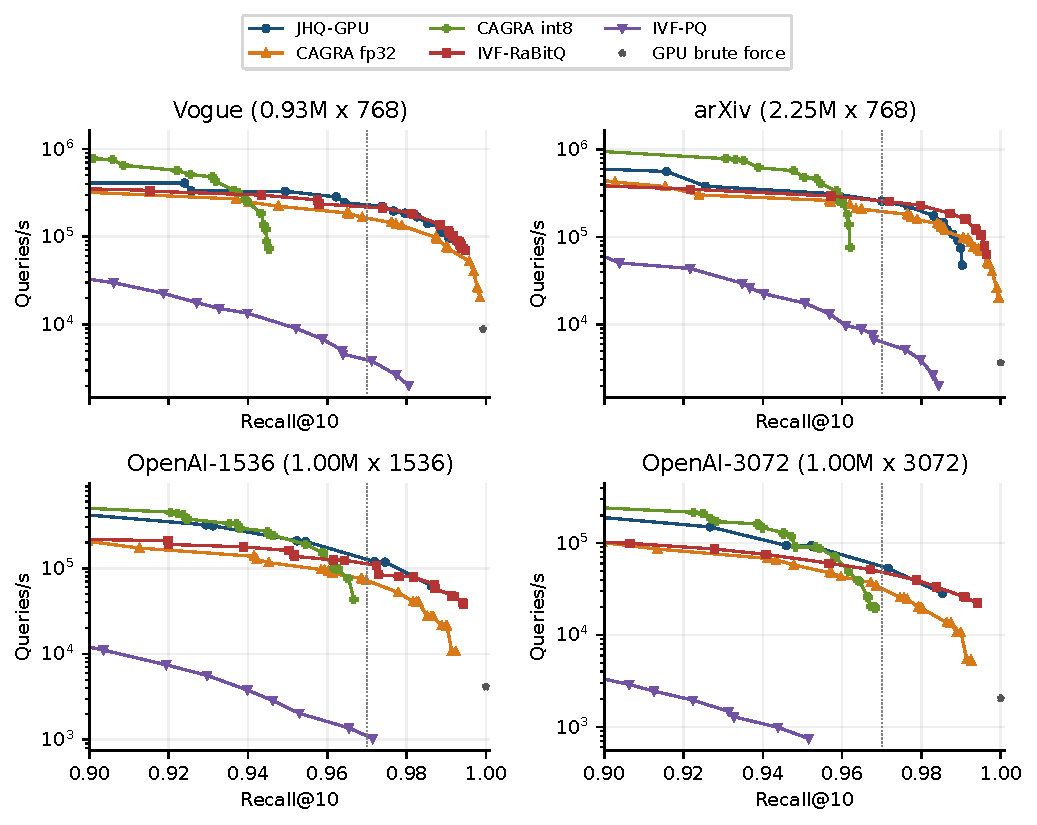
\includegraphics[width=\linewidth]{ch7/frontiers.pdf}
\caption[Main-comparison recall--throughput frontiers]{Measured host-to-host recall--QPS frontiers on the four main-comparison datasets.
The displayed recall window begins at 0.90, with a vertical line at 0.97;
all baseline families,
including CAGRA int8, participate in frontier construction. Lines connect
measured points; throughput uses a logarithmic axis.}
\label{fig:7-frontiers}
\end{figure}

\subsection{Throughput at matched recall}

The lead over CAGRA fp32 holds under both estimators, while the much
smaller arXiv--RaBitQ margin changes direction
(\cref{tab:7-matched}). The interpolated and qualifying-measured
estimators follow \cref{sec:3-4}.

\par\medskip\noindent\begin{minipage}{\linewidth}
\captionsetup{hypcap=false}
\centering
\captionof{table}[Cross-system comparison at recall 0.97]{Recall 0.97 comparison. Each ratio is interpolated / measured;
values above one favour JHQ. JHQ kQPS is the interpolated estimate.
The small arXiv--RaBitQ difference changes direction with the estimator.}
\label{tab:7-matched}
\small\setlength{\tabcolsep}{4pt}
% Generated by scripts/build_ch7.py; do not edit numbers manually.
\begin{tabular}{@{}lrrr@{}}
\toprule
Dataset & JHQ kQPS & vs CAGRA fp32 & vs IVF-RaBitQ \\
\midrule
Vogue & 230.8 & 1.416 / 1.537 & 1.059 / 1.046 \\
arXiv & 258.6 & 1.317 / 1.422 & 0.996 / 1.015 \\
OpenAI-1536 & 126.7 & 1.747 / 2.294 & 1.130 / 1.111 \\
OpenAI-3072 & 55.9 & 1.747 / 2.088 & 1.157 / 1.346 \\
\bottomrule
\end{tabular}

\end{minipage}\par\medskip

Vogue's modest RaBitQ lead depends on grouped execution. At fixed
index, probes, budget and final outputs, replacing the grouped path by
one block lowers the recall-0.97 JHQ/RaBitQ ratio from 1.059 to 0.933
at batch 1,000. CAGRA int8 is $1.20$--$1.98\times$ faster at recall
0.90--0.92 but cannot reach 0.97 within its tested grid. RaBitQ leads
at some targets above 0.98, and CAGRA fp32 leads near 0.99 on arXiv
(\cref{fig:7-frontiers}).

\subsection{Precision sensitivity on the OpenAI datasets}
\label{sec:7-precision}

Using FP32 in place of TF32 reduces throughput by about 5\% at matched
configurations, while the checked FP32 frontiers retain their lead over
CAGRA fp32. Source inspection found that the main implementation uses
TF32 multiplication with FP32 accumulation for OpenAI rotation and
centroid matrix products (\cref{sec:4-2}). The precision check
changes that arithmetic switch and alternates the two variants across
probe settings: 37 OpenAI-1536 and 39 OpenAI-3072 configurations, five
rounds each at batch 1,000. Both reuse one TF32-trained model; add and
query arithmetic, including encoding and routing, change. This is not
independent FP32 retraining.

\par\medskip\noindent\begin{minipage}{\linewidth}
\centering\captionsetup{hypcap=false}
\captionof{table}[FP32 sensitivity at matched configurations]{FP32 sensitivity. QPS ratio is FP32/TF32 at equal configuration
(geometric mean); recall differences have the same direction. The last
two columns compare the FP32 frontier at recall 0.97 with archived
IVF-RaBitQ and CAGRA fp32 frontiers. The precision check reuses baseline measurements from the main comparison.}
\label{tab:7-precision}
\scriptsize\setlength{\tabcolsep}{3pt}
\begin{tabular}{@{}lrrrrr@{}}
\toprule
Dataset & Pairs & QPS ratio & $\Delta$Recall & vs RaBitQ & vs CAGRA \\
\midrule
OpenAI-1536 & 37 & 0.953 & +0.0003--+0.0005 & 1.086 & 1.679 \\
OpenAI-3072 & 39 & 0.951 & +0.0000--+0.0003 & 1.079 & 1.629 \\
\bottomrule
\end{tabular}

\end{minipage}\par\medskip

At matched configuration, recall increases by 0--0.0005. At recall 0.97,
FP32 is about 3\% slower than TF32 measured alongside it, but its ratios
to archived RaBitQ are 1.086 on OpenAI-1536 and 1.079 on OpenAI-3072;
ratios to archived CAGRA fp32 are 1.679 and 1.629. The repeated original
variant gives RaBitQ ratios of 1.118 and 1.114, compared with historical
1.130 and 1.157. \Cref{fig:7-precision} shows this paired precision
comparison; the next check remeasures the baselines.

\par\medskip\noindent\begin{minipage}{\linewidth}
\captionsetup{hypcap=false}
\centering
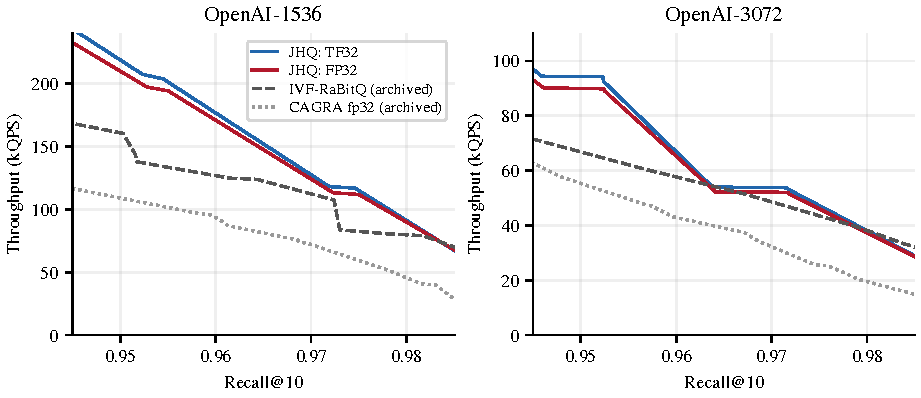
\includegraphics[width=\linewidth]{variants/final-polish/figures/precision.pdf}
\captionof{figure}[TF32 and FP32 precision frontiers]{Precision check. Solid curves are JHQ variants measured together;
dashed/dotted baselines come from the main comparison.
All use the chapter's frontier and interpolation rules.}
\label{fig:7-precision}
\end{minipage}\par\medskip

\subsection{Baselines remeasured with JHQ}
\label{sec:b-precision-anchors}

The same-session check confirms an FP32 lead at recall 0.97 under
both estimators in its tested grid. \Cref{tab:b-precision-anchors}
reports ratios to both RaBitQ and CAGRA fp32.

Twelve paired configurations per OpenAI dataset use the main
comparison's memory-pool settings. Two five-round JHQ repetitions
bracket the baseline runs, and their median rates are combined
geometrically. Equal-configuration FP32/TF32 means are 0.956 for
OpenAI-1536 and 0.964 for OpenAI-3072. Both variants reuse TF32-trained
caches and change only add/query arithmetic.

\par\medskip\noindent\begin{minipage}{\linewidth}
\captionsetup{hypcap=false}
\centering
\captionof{table}[Baselines remeasured with JHQ]{The same-session check at recall 0.97, batch 1,000. Baseline ratios are interpolation / strict measured threshold; FP32/TF32 is interpolated. All methods were remeasured together; the precision check instead reuses the main comparison's baselines.}
\label{tab:b-precision-anchors}
\footnotesize\setlength{\tabcolsep}{3pt}
\begin{tabular}{@{}lrrr@{}}
\toprule
Dataset & FP32/TF32 at 0.97 & FP32 / RaBitQ & FP32 / CAGRA \\
\midrule
OpenAI-1536 & 0.980 & 1.126 / 1.053 & 1.752 / 1.633 \\
OpenAI-3072 & 0.973 & 1.328 / 1.316 & 1.825 / 2.019 \\
\bottomrule
\end{tabular}

\end{minipage}\par\medskip

The check covers a limited grid near recall 0.97. OpenAI-3072's RaBitQ
bracket spans recall 0.9669--0.9796, so the size of the margin depends
on grid coverage and estimator. It is evidence for this local comparison,
not for independently FP32-trained frontiers or every recall target.


\subsection{Interpreting the OpenAI comparison}

The two OpenAI exports provide a useful dimension comparison because
both derive from Qdrant's DBpedia embeddings
\cite{data_openai1536,data_openai3072}. Alignment was checked before
interpreting their different widths: after truncation and
renormalisation, all 1,000 query rows and 10,299 sampled database rows
have cosine $\geq0.9980$, with median 1.000000; their ground-truth sets
share 9.046 of ten neighbours on average. These checks support row
alignment without establishing a complete original-entity-ID join.
Doubling dimension leaves the CAGRA fp32 ratio at 1.747 and changes the
RaBitQ ratio from 1.130 to 1.157, so dimension alone does not explain
the observed advantage.

At 128 probes, larger gains accompany smaller refinement multipliers:
4--8 on OpenAI, 64 on Vogue and 100 on arXiv, whose later full-pool
calibration selects 200. This is an association across workloads,
not a controlled causal comparison; \cref{sec:8-centring} tests one
representation-level explanation. Small margins and measurement
sensitivity are examined in \cref{sec:7-8}.

\subsection{Small batches change the competitive region}
\label{sec:7-smallbatch}

At batch 8 and recall 0.97, CAGRA fp32 is faster on all four datasets
under both estimators. JHQ remains competitive at lower recall, but
near ties depend on how measured endpoints are used. The small-batch
study compares scheduled JHQ, CAGRA fp32/int8 and IVF-RaBitQ at
batches 8 and 32 on the four main-comparison datasets. Five synchronous
host-to-host rounds use 1,000 and 992 queries, respectively. The
1,808 measurements include a one-block JHQ control; IVF-PQ and brute
force are outside this study.

\suppressfloats[t]
\par\medskip\noindent\begin{minipage}{\linewidth}
\captionsetup{hypcap=false}
\centering
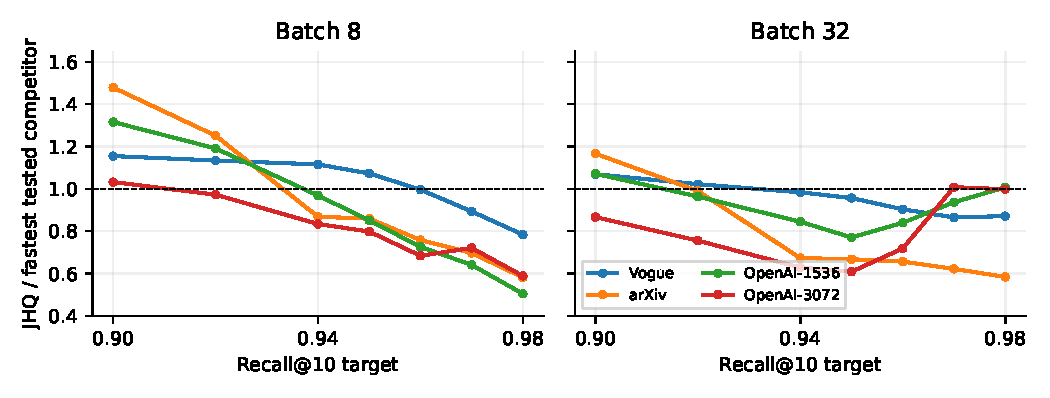
\includegraphics[width=\linewidth]{t4-t5/smallbatch.pdf}
\captionof{figure}[Small-batch competitive regions]{Small-batch JHQ / fastest-competitor
QPS under interpolation with qualifying measured endpoints. Above one
favours JHQ. \Cref{tab:7-smallbatch} gives strict thresholds.}
\label{fig:7-smallbatch}
\end{minipage}\par\medskip

\par\medskip\noindent\begin{minipage}{\linewidth}
\captionsetup{hypcap=false}
\centering
\captionof{table}[Small-batch matched-recall ratios]{Small-batch QPS ratios:
interpolation with qualifying endpoints / strict measured threshold.
The fastest competitor is selected independently for each estimator;
higher-recall qualifying endpoints remain eligible without extrapolation.}
\label{tab:7-smallbatch}
\footnotesize\setlength{\tabcolsep}{4pt}
\begin{tabular}{@{}lrrrr@{}}
\toprule
Dataset & $b$ & $R=0.90$ & $R=0.95$ & $R=0.97$ \\
\midrule
Vogue & 8 & 1.155 / 1.091 & 1.073 / 0.980 & 0.893 / 0.854 \\
Vogue & 32 & 1.069 / 0.997 & 0.956 / 0.895 & 0.865 / 0.839 \\
arXiv & 8 & 1.479 / 1.454 & 0.859 / 0.851 & 0.697 / 0.698 \\
arXiv & 32 & 1.166 / 1.148 & 0.667 / 0.661 & 0.622 / 0.582 \\
OpenAI-1536 & 8 & 1.316 / 1.131 & 0.851 / 0.825 & 0.641 / 0.620 \\
OpenAI-1536 & 32 & 1.071 / 0.915 & 0.770 / 0.752 & 0.937 / 0.914 \\
OpenAI-3072 & 8 & 1.032 / 0.953 & 0.798 / 0.798 & 0.721 / 0.702 \\
OpenAI-3072 & 32 & 0.866 / 0.734 & 0.608 / 0.771 & 1.008 / 1.351 \\
\bottomrule
\end{tabular}

\end{minipage}\par\medskip

At recall 0.97, interpolated JHQ/fastest-competitor ratios are
0.641--0.893 for batch 8 and 0.622--1.008 for batch 32.
OpenAI-3072 favours JHQ under the batch-32 measured threshold, while
Vogue's batch-8 lead at recall 0.95 requires interpolation
(\cref{tab:7-smallbatch}).

At recall 0.90, interpolation with qualifying endpoints favours JHQ
by 1.032--1.479 at batch 8; the strict threshold gives only three
wins. Batch-32 ratios range from 0.866 to 1.166, with one strict win.
Scheduling gives $1.7$--$3.3\times$ over one block at recall 0.95,
which improves JHQ's execution without ensuring a cross-system lead.

The boundary includes interface costs. Null calls containing transfers
and synchronisation take median 0.012--0.072\,ms; this cost remains in
the search timings. CAGRA uses Python and JHQ/RaBitQ use C++, with
warm-up conventions recorded in \cref{sec:a-t4-t5}.


\subsection{Historical comparison with the CPU implementation}
\label{sec:7-cpu}

An earlier comparison with the JHQ authors' CPU implementation found
GPU/CPU throughput ratios of 52--85 on Vogue, 56--98 on arXiv,
85--108 on OpenAI-1536 and 75--77 on OpenAI-3072 at matched recall.
It ran on the same server's Xeon Platinum 8470Q using local compatibility
and Recall@10 fixes to the CPU artifact. The plotted CPU frontier uses
the faster of 16 and 32 threads on Vogue and OpenAI-3072, and 32 threads
on the other two datasets. It sweeps
$\alpha\in\{2,4,8,16,32,100\}$ and 128--1,024 probes; smaller probe
counts are excluded because thread-startup overhead distorts timing.
Ratios use log-throughput interpolation at equal recall.

These are historical implementation comparisons. The GPU runs use the earlier implementation,
CPU codebooks are trained separately, and the OpenAI CPU indexes have
4,096 lists rather than the GPU's 8,192. Most CPU settings were timed
once. A later October CPU refinement study also uses unmatched settings:
Vogue has 1,024 lists and $[8,4]$ bits rather than the main comparison's
4,096 lists. A hardware-speedup claim for the evaluated GPU version
still requires matched index and timing controls.

\section{Cartesian LUT, Packed Loads and Lane Refinement}
\label{sec:7-3}


\subsection{LUT factorisation and throughput}

Two 16-entry tables are the fastest tested form in 22 of 24 settings,
but factorisation in real arithmetic does not imply identical FP32
scores or final IDs. \Cref{fig:7-lut} tests six datasets, probe counts
8, 32, 128 and 512, fixed $\alpha=100$, and
$\glut\in\{1,2,4,8\}$. Five rounds use batch 1,000, or 999 for Stella.
The exceptions are near ties: one group is 0.23\% faster on arXiv at
128 probes, and four groups are 0.84\% faster on OpenAI-3072 at eight
probes. Two groups beat one in 23 of 24 paired settings; dataset
geometric-mean ratios range from 1.021 to 1.318.

\begin{figure}[!htbp]
\centering
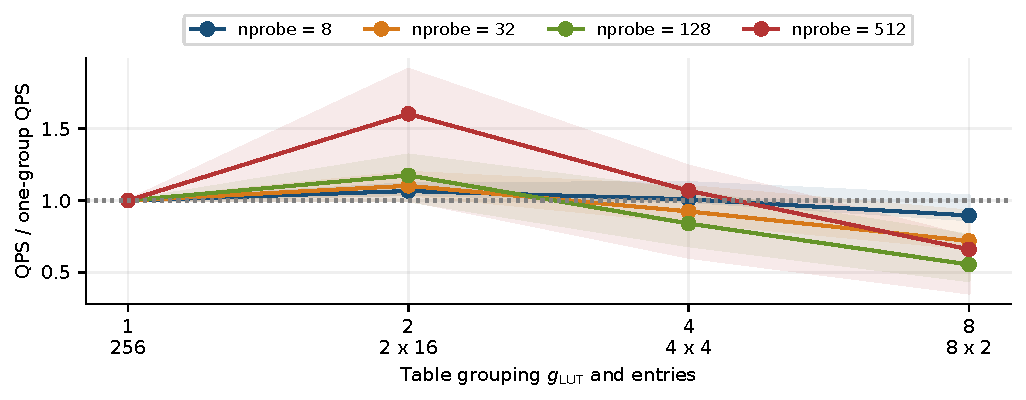
\includegraphics[width=\linewidth]{ch7/lutgroups.pdf}
\caption[Cartesian lookup-table grouping]{Cartesian table grouping at fixed $\alpha=100$.
Group counts describe $\glut$, not parallel scan groups. Curves are medians
of per-dataset QPS ratios to the one-group reference; shading shows their range.}
\label{fig:7-lut}
\end{figure}

Individual two-group/one-group ratios range from $0.998$ to
$1.914$. Four and eight groups each store 16 entries per subspace but
require more lookups and additions; their smaller tables do not always
pay off. Occupancy and instruction costs were not isolated. Across each
four-variant setting, the largest reported recall spread is $10^{-4}$.

The strict score check compares identical candidates on Vogue, arXiv
and OpenAI-3072 at 128 probes and $\alpha=100$. Full and $16+16$ tables
produce different bits for 22.6--26.1\% of scores, with maximum relative
error $4.53\times10^{-7}$. Across all table forms, 20.5--29.4\% differ
and the maximum error is $4.63\times10^{-7}$. Vogue's final IDs differ
on two to four of 256 queries; arXiv and OpenAI do not differ. Even an
unchanged shortlist can yield different final IDs because its rounded
primary scores enter refinement (\cref{sec:a-t4-t5}).

\subsection{Packed access and cooperative residual scoring}

Word-packed access improves throughput by $1.012$--$1.658\times$ in
48 matched comparisons across six datasets, four probe counts and
$\glut\in\{1,2\}$, with recall differences at most $10^{-4}$.
Both layouts are subspace-major; the change combines word loading and
unpacking (\cref{fig:7-packing-refinement}).

The refinement controls separate wider loads from cooperation. L0 is
the scalar reference, L1 changes only its load path, and L16 assigns
16 lanes to one candidate. Variant order rotates across five rounds,
with three searches per variant per round. L16 gives
$1.015$--$1.789\times$ end-to-end gains in the twelve ordinary settings;
the separate high-budget arXiv control at $\alpha=200$ reaches
$2.383\times$ (\cref{tab:7-refinement}).

\begin{figure}[!htbp]
\centering
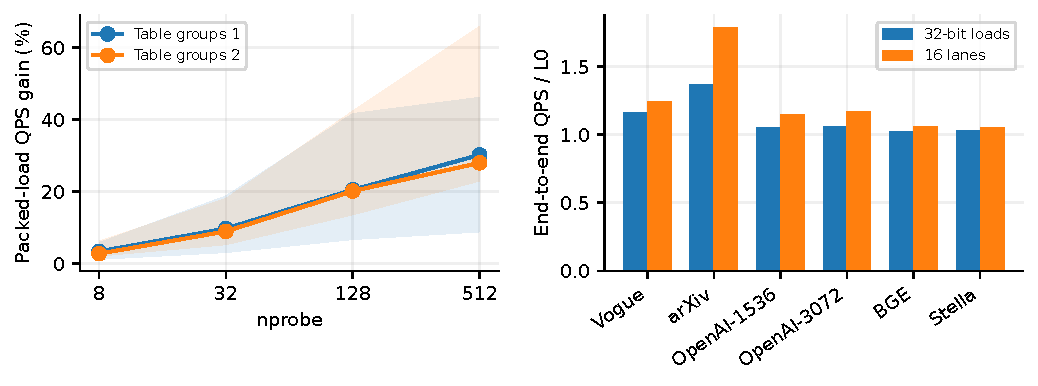
\includegraphics[width=\linewidth]{ch7/packing_refinement.pdf}
\caption[Packed access and refinement controls]{Packing and refinement controls. Left: median packed-load QPS
 gain across six datasets, with shaded minimum--maximum ranges, for each
 table grouping and probe count. Right: measured load-only and 16-lane
 end-to-end gains at 128 probes and the ordinary dataset-specific budgets.
 Panels use different experiment families.}
\label{fig:7-packing-refinement}
\end{figure}

\begin{table}[!htbp]
\centering
\caption[Refinement gains at 128 probes]{Refinement at 128 probes. Ratios are paired end-to-end gains over
 L0, except the last column, which is the profiled refinement-kernel gain.
 The kernel and application gains must not be interchanged.}
\label{tab:7-refinement}
\small\setlength{\tabcolsep}{4pt}
% Generated by scripts/build_ch7.py; do not edit numbers manually.
\begin{tabular}{@{}lrrrr@{}}
\toprule
Dataset & $\alpha$ & $L1/L0$ QPS & $L16/L0$ QPS & Kernel gain \\
\midrule
arXiv & 100 & 1.368 & 1.789 & 5.97 \\
BGE & 32 & 1.026 & 1.062 & 1.97 \\
OpenAI-1536 & 8 & 1.055 & 1.145 & 3.34 \\
OpenAI-3072 & 4 & 1.063 & 1.171 & 8.81 \\
Stella & 16 & 1.030 & 1.053 & 2.66 \\
Vogue & 64 & 1.161 & 1.240 & 3.72 \\
\bottomrule
\end{tabular}

\end{table}

A simple stage-share model closely predicts the end-to-end gains.
Load-only L1 preserves L0's bits and gains $1.368\times$ on arXiv.
With lane cooperation at $\alpha=100$, arXiv refinement falls from
4,277.5 to 716.8\,$\mu$s, a $5.97\times$ kernel gain but
$1.789\times$ overall. OpenAI-3072 similarly gives $8.81\times$
in the kernel and $1.171\times$ overall. For baseline wall-time fraction
$f$ and refinement speedup $s$,
\[
 \frac{T'}T=(1-f)+\frac f s,\qquad
 \frac T{T'}=\frac1{1-f+f/s}.
\]
Using $f=0.529$ on arXiv predicts $1.787\times$, compared with measured
$1.789\times$; using $f=0.168$ on OpenAI-3072 predicts
$1.175\times$, compared with $1.171\times$. Other stages limit the
benefit, and separate stage profiling makes this an explanatory model.
Lane regrouping changes FP32 addition order, with relative distance
error up to $\approx1.6\times10^{-6}$ and occasional ordering changes;
the result is a speed improvement, not universal bit identity.

\section{Selection Correctness and Performance}
\label{sec:7-4}


\subsection{Strict CPU reference for computed-score selection}
\label{sec:7-strict-selection}

All 55,296 grouped query instances exactly match the CPU reference's
primary order. One-block selection satisfies distance order throughout,
with 56 set differences confined to tied cut-offs; the final selection
of retained refined scores is exact in all 69,120 instances
(\cref{tab:7-strict-selection}).

The strict selection check sorts GPU-produced scores by
$(\primarydist,\mathrm{position})$. Its exporter follows the scan layout
and accumulation order, and exported scores for valid returned candidates
match bitwise. Source comparison finds only export changes from the
table-sweep version. The 270 configurations cover Vogue, arXiv and
OpenAI-3072, probes 1, 8 and 128, $\alpha\in\{4,100,200\}$,
$\gscan\in\{0,1,2,4,8\}$ and both bound settings.

\suppressfloats[t]
\begin{table}[!htbp]
\centering
\caption[Strict computed-score selection checks]{Strict selection checks against a CPU reference.
Set and order equality use the complete primary key. Valid count checks
$\min(c,n_c)$ survivors; final equality sorts retained computed refined
scores by $(\refineddist,\mathrm{ID})$, including their FP32 bits. Counts
are query instances, with queries reused across configurations.}
\label{tab:7-strict-selection}
\footnotesize\setlength{\tabcolsep}{3pt}
\begin{tabular}{@{}lrrrrr@{}}
\toprule
Path & Queries & Set / order exact & Tie-only & Valid count & Final exact \\
\midrule
$\gscan\geq1$ & 55,296 & 55,296 / 55,296 & 0 & 55,296 & 55,296 \\
$\gscan=0$ & 13,824 & 13,768 / 8,758 & 56 & 13,824 & 13,824 \\
\bottomrule
\end{tabular}

\end{table}

All 19,120 underfull cases have the correct valid-candidate count.
These results test \cref{lem:5-buffer,prop:5-local-coverage,prop:5-shared-bound}
for the recorded cases. Final-selection equality concerns retained
computed scores, not original-space exact neighbours; sanitizer coverage
is limited to its recorded subsets (\cref{sec:a-t4-t5}).


\subsection{Shared bounds preserve the selection target}

Enabling the shared bound preserves the checked outputs in all
48 settings, with throughput ratios of $0.994$--$1.562\times$.
The gain comes from less selection and merge maintenance after a useful
bound is available. On arXiv at $\alpha=200$, batch 1,000 and eight
groups, merge time falls from 2,629 to 471\,$\mu$s and scan time from
7,968 to 5,513\,$\mu$s. Slight regressions in some settings show that
the mechanism's overhead can still outweigh its savings.

\subsection{Probe selection and output consistency}

Radix selection returns the same computed-score probes in all 1,792
synthetic cases. On all 1,000 queries in each of arXiv, Vogue and OpenAI-3072,
probe IDs, primary scores and primary positions also match the reference.
The change selects among existing centroid scores; it does not change
their arithmetic or the OpenAI precision mode
(\cref{sec:7-precision}).

\par\medskip\noindent\begin{minipage}{\linewidth}
\captionsetup{hypcap=false}
\centering
\captionof{table}[Probe-selection throughput ratios]{End-to-end throughput ratios for radix versus the earlier probe selector for the exact computed-score probe
 change. Each workload--batch comparison has ten timing rounds per binary,
 collected in alternating runs. Ratios $>1$ favour radix selection.}
\label{tab:7-probe}
\small
% Generated by scripts/build_ch7.py; do not edit numbers manually.
\begin{tabular}{@{}lrrrr@{}}
\toprule
Dataset & Batch 8 & 32 & 256 & 1,000 \\
\midrule
arXiv & 1.074 & 1.063 & 1.035 & 1.034 \\
Vogue & 1.109 & 1.103 & 1.052 & 1.041 \\
OpenAI-3072 & 1.167 & 1.117 & 1.055 & 1.050 \\
\bottomrule
\end{tabular}

\end{minipage}\par\medskip

The end-to-end gain is $1.034$--$1.167\times$
(\cref{tab:7-probe}). At batch 8, the profiled probe stage falls from
56.5 to 22.6\,$\mu$s on arXiv, 52.7 to 14.7\,$\mu$s on Vogue, and
77.8 to 16.7\,$\mu$s on OpenAI-3072. These stage savings are a smaller
fraction of full-batch time. The unresolved Vogue difference between
processes is discussed separately in \cref{sec:7-8}.

\section{Held-out Budget Quality, Throughput and Payback}
\label{sec:7-5}

Full-pool calibration meets the held-out quality target in all twelve
tested settings; 128-query calibration costs less but can miss it often.
The controls use fixed
$\alpha=100$ and $\alpha=64$; \cref{ch:refinement} defines the rule.

\subsection{Unlabelled selection and a labelled diagnostic oracle}

The six datasets are tested at 128 and 512 probes. Full-pool calibration
uses all 500 calibration queries; sampled calibration uses 64 subsets at
each sample size from the disjoint pools in \cref{sec:3-2}. Enumeration
checks the same rule across every tested budget, while a diagnostic
oracle uses held-out labels to identify a qualifying budget
(\cref{sec:6-4,tab:6-controls}). All rule variants use
\cref{eq:6-agreement} with $k=10$ and $\epsilon=1$; labels evaluate the
selected budget rather than guide its calibration.

\subsection{Full-pool calibration as the quality-first working point}

With all 500 calibration queries, the largest observed held-out loss
is 0.0006, below the $10^{-3}$ target in all twelve settings.
Throughput is 0.908--1.000 of the labelled oracle's rate, and calibration
costs 9.5--60.3\,ms (\cref{tab:7-budget-full}). The geometric-mean rate
ratio to fixed 100 is $1.111\times$ over all settings, or
$1.193\times$ over the ten where fixed 100 also meets the quality target.
Against fixed 64, calibration is faster in six settings, equal in two
and slower in four. Its main benefit is the observed coverage of the
twelve quality targets, not a guarantee for future query distributions.

\begin{table}[!htbp]
\centering
\caption[Full-pool budget calibration]{Full-pool calibration ($S=500$). Loss is relative to the best
measured held-out recall; rates are kQPS from the selected fixed budget.
``Cal.'' is one full-pool calibration call per setting, not a repeated
stream timing. Held-out counts are 500, or 499 for Stella.}
\label{tab:7-budget-full}
\footnotesize\setlength{\tabcolsep}{3pt}
% Generated by scripts/build_ch7.py; do not edit numbers manually.
\begin{tabular}{@{}lrrrrrrr@{}}
\toprule
Dataset & Probe & $\alpha_{\rm full}$ & Loss & $Q_{\rm full}$ & vs 100 & vs oracle & Cal. ms \\
\midrule
Vogue & 128 & 100 & 0.0000 & 202.9 & 1.000 & 0.908 & 10.1 \\
arXiv & 128 & 200 & 0.0000 & 151.5 & 0.728 & 1.000 & 10.0 \\
OpenAI-1536 & 128 & 8 & 0.0000 & 267.7 & 1.599 & 1.000 & 9.5 \\
OpenAI-3072 & 128 & 4 & 0.0000 & 145.0 & 1.691 & 1.000 & 17.1 \\
BGE & 128 & 64 & 0.0006 & 124.9 & 1.075 & 0.932 & 17.1 \\
Stella & 128 & 16 & 0.0006 & 110.4 & 1.153 & 1.000 & 20.6 \\
Vogue & 512 & 100 & 0.0002 & 100.1 & 1.000 & 0.969 & 20.9 \\
arXiv & 512 & 200 & 0.0000 & 69.0 & 0.831 & 1.000 & 25.1 \\
OpenAI-1536 & 512 & 8 & 0.0000 & 114.9 & 1.326 & 1.000 & 21.8 \\
OpenAI-3072 & 512 & 4 & 0.0002 & 52.1 & 1.219 & 0.977 & 40.5 \\
BGE & 512 & 64 & 0.0006 & 50.8 & 1.033 & 1.000 & 42.3 \\
Stella & 512 & 16 & 0.0006 & 36.0 & 1.041 & 1.000 & 60.3 \\
\bottomrule
\end{tabular}

\end{table}

\subsection{Lower-cost sampling and its quality risk}

A typical selected budget can look appropriate while individual samples
fail the quality target. At $S=128$, the median budget matches the
labelled oracle in ten of twelve settings, differing on arXiv at
128 probes and OpenAI-3072 at 512. Selected budgets span 4--200 across
workloads (\cref{tab:7-budget-quality}).

\begin{table}[!htbp]
\centering
\caption[Sampled-budget held-out quality]{Held-out quality at $S=128$. Rule $\alpha$ is the median across
64 calibration samples; oracle $\alpha$ uses held-out labels. $\overline R_{\rm rule}$
is reconstructed mean recall. ``Losses'' counts samples with recall loss
$>10^{-3}$ relative to the best tested held-out recall; $L_{95}$ is the
logged lower-order 95th-percentile loss estimate. $R_{100}$ is
fixed-budget recall.}
\label{tab:7-budget-quality}
\small\setlength{\tabcolsep}{3pt}
% Generated by scripts/build_ch7.py; do not edit numbers manually.
\begin{tabular}{@{}lrrrrrr@{}}
\toprule
Dataset & Probe & $\alpha$: rule/oracle & $R_{100}$ & $\overline{R}_{\rm rule}$ & Losses & $L_{95}$ \\
\midrule
Vogue & 128 & 64 / 64 & 0.9680 & 0.9677 & 5/64 & 0.0022 \\
arXiv & 128 & 100 / 200 & 0.9748 & 0.9751 & 40/64 & 0.0024 \\
OpenAI-1536 & 128 & 8 / 8 & 0.9280 & 0.9279 & 4/64 & 0.0000 \\
OpenAI-3072 & 128 & 4 / 4 & 0.9252 & 0.9252 & 0/64 & 0.0000 \\
BGE & 128 & 32 / 32 & 0.9198 & 0.9190 & 1/64 & 0.0008 \\
Stella & 128 & 16 / 16 & 0.9892 & 0.9884 & 6/64 & 0.0030 \\
Vogue & 512 & 64 / 64 & 0.9916 & 0.9915 & 2/64 & 0.0002 \\
arXiv & 512 & 200 / 200 & 0.9878 & 0.9885 & 32/64 & 0.0016 \\
OpenAI-1536 & 512 & 8 / 8 & 0.9740 & 0.9738 & 4/64 & 0.0000 \\
OpenAI-3072 & 512 & 4 / 8 & 0.9704 & 0.9702 & 0/64 & 0.0002 \\
BGE & 512 & 64 / 64 & 0.9670 & 0.9661 & 24/64 & 0.0014 \\
Stella & 512 & 16 / 16 & 0.9954 & 0.9945 & 7/64 & 0.0030 \\
\bottomrule
\end{tabular}

\end{table}

ArXiv exceeds the target in 40 of 64 samples at 128 probes and 32 of
64 at 512 probes, despite mean loss of 0.0009. Its fixed-100 losses are
0.0012 and 0.0016, respectively, so improving the inherited budget does
not by itself meet the target. BGE at 512 probes has 24 failures and
$L_{95}=0.0014$; Stella's $L_{95}$ reaches 0.0030, while OpenAI-3072 has
no recorded failures (\cref{tab:7-budget-quality}). Maximum individual
losses are 0.0050 on arXiv and 0.0046 on BGE, both at 512 probes.

\begin{figure}[!htbp]
\centering
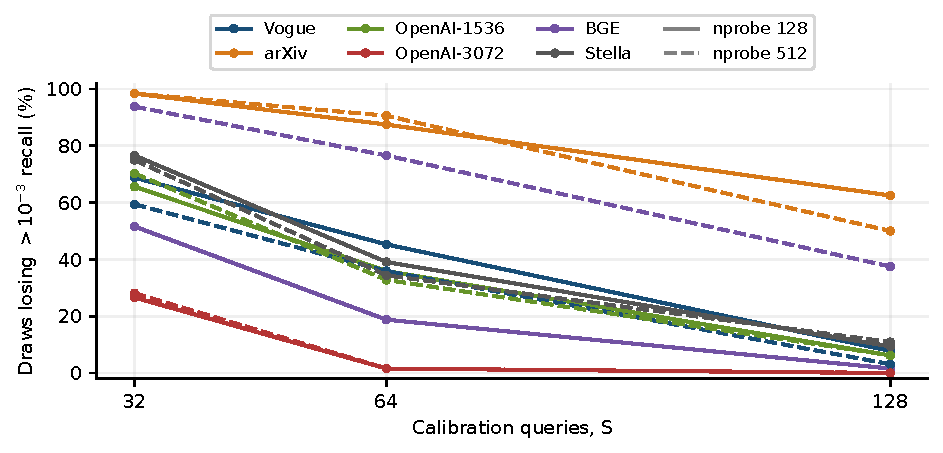
\includegraphics[width=0.82\linewidth]{ch7/budget_risk.pdf}
\caption[Held-out risk across sample sizes]{Held-out risk across sample sizes. The vertical axis is the
percentage of calibration samples losing more than $10^{-3}$ held-out recall
relative to the best tested budget. Increasing $S$ also tightens the allowed
slot-disagreement fraction because \cref{eq:6-agreement} keeps threshold one.}
\label{fig:7-budget-risk}
\end{figure}

\subsection{Estimated throughput and calibration economics}

Sampling often selects a faster budget, but these speed estimates must
be read alongside the preceding quality results. Using the mean
selected-budget estimate in \cref{sec:a-budget-contract}, $S=128$ exceeds
fixed-100 QPS in ten settings by $1.028$--$1.691\times$. ArXiv ratios
are 0.908 and 0.917, with better mean recall but no throughput payback.
Against fixed 64, sampling wins nine of twelve settings, with geometric
mean $1.054\times$ and range $0.821$--$1.367\times$; on OpenAI the range
is $1.052$--$1.367\times$. Both fixed controls fail arXiv's quality
target, so the complete ranking is not uniformly quality-matched.

\begin{table}[!htbp]
\centering
\caption[Sampled-calibration economics]{Calibration economics, $S=128$. Rates are kQPS and rule rate is
mean selected-budget QPS. Ratios compare with fixed 100 and fixed 64.
The ``Batches'' column gives payback relative to fixed 100 using 500
queries, or 499 for Stella; ``Never'' denotes no throughput payback.
The quality column separately marks whether fixed 100 meets the
held-out loss target.}
\label{tab:7-budget-cost}
\footnotesize\setlength{\tabcolsep}{3pt}
% Generated by scripts/build_ch7.py; do not edit numbers manually.
\begin{tabular}{@{}lrrrrrr@{}}
\toprule
Dataset & Probe & $Q_{100}$ & $\overline Q_{\rm rule}$ & Ratio & Cal. ms & Batches \\
\midrule
Vogue & 128 & 202.9 & 224.4 & 1.106 & 4.0 & 17.0 \\
arXiv & 128 & 207.9 & 188.8 & 0.908 & 4.2 & Never \\
OpenAI-1536 & 128 & 167.5 & 268.5 & 1.603 & 3.9 & 3.5 \\
OpenAI-3072 & 128 & 85.7 & 145.0 & 1.691 & 5.7 & 2.4 \\
BGE & 128 & 116.2 & 131.2 & 1.130 & 6.5 & 13.2 \\
Stella & 128 & 95.7 & 110.3 & 1.153 & 7.5 & 10.8 \\
Vogue & 512 & 100.1 & 102.9 & 1.028 & 7.5 & 55.4 \\
arXiv & 512 & 83.1 & 76.2 & 0.917 & 9.7 & Never \\
OpenAI-1536 & 512 & 86.6 & 115.0 & 1.327 & 8.8 & 6.2 \\
OpenAI-3072 & 512 & 42.8 & 52.1 & 1.219 & 13.1 & 6.2 \\
BGE & 512 & 49.2 & 51.1 & 1.039 & 15.8 & 41.2 \\
Stella & 512 & 34.6 & 36.0 & 1.041 & 21.3 & 37.1 \\
\bottomrule
\end{tabular}

\end{table}

Sampled calibration costs 3.9--21.3\,ms. The largest positive modelled
paybacks are 0.54\,s against fixed 100 and 2.72\,s against fixed 64;
full-pool calibration gives 1.52 and 2.25\,s, respectively
(\cref{sec:6-5,eq:6-payback,tab:7-budget-cost}). The direct reuse tests
below then measure both total cost and achieved quality.

\subsection{Complete decision traces and finite-pool risk}
\label{sec:7-budget-trace}

Replaying the recorded calibration choices confirms the finite-pool
calculation: all 2,304 sampled decisions and twelve full-pool decisions
match enumeration. Their recorded discrepancy curves are monotone, and
summing per-query counts reproduces all 18,432 tested grid counts
(\cref{eq:6-finite-pool}). This validates the observed traces; it does
not establish nesting for every distance-tied subset or query ordering
(\cref{sec:6-3}).

At $S=32$, maximum individual loss reaches 0.0294, versus at most
0.0006 for full-pool calibration.

For arXiv at 128 probes, the predicted and observed probabilities of
exceeding the loss target are 0.965 versus 0.984 with $S=32$,
0.875 versus 0.875 with $S=64$, and 0.620 versus 0.625 with $S=128$
(\cref{fig:7-finite-pool}). The largest of 36 gaps occurs on BGE at
512 probes: 0.519 predicted versus 0.375 observed, a difference of
0.144. These predictions concern samples from the fixed calibration
pool, using each selected budget's measured held-out quality; calibration
itself uses no labels.

\begin{figure}[!htbp]
\centering
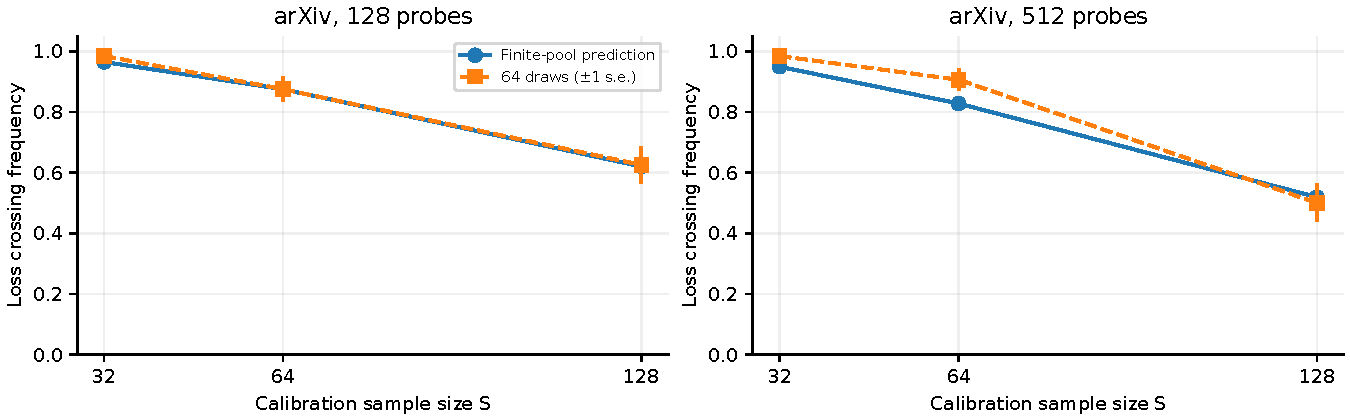
\includegraphics[width=\linewidth]{supplement/finite-pool.pdf}
\caption[Finite-pool risk prediction and observation]{Finite-pool prediction and observed arXiv quality-target violations. Bars
show one estimated standard error over 64 independently drawn subsets
conditional on the fixed pool, not uncertainty over future workloads.}
\label{fig:7-finite-pool}
\end{figure}

Ten alternating timing repeats show a low-budget plateau, rather than
a general rule that each smaller budget is faster.

\subsection{Direct calibration-plus-reuse measurement}
\label{sec:7-stream-cost}

Four settings compare fixed budgets 64 and 100,
128-query calibration and full-pool calibration across five rotated
rounds of 500 reuse batches. Every batch repeats the same held-out query
pool. This measures amortisation on a stable workload, not performance
under new-query arrivals or drift. Timing includes sample gathering,
calibration, budget installation and initial graph setup, but excludes
construction, warm-up and scan-scheduler calibration.

\par\medskip\noindent\begin{minipage}{\linewidth}
\centering\captionsetup{hypcap=false}
\captionof{table}[Direct costs for 500 reuse batches]{Direct total milliseconds for 500 reuse batches, averaged over
five rounds, including budget calibration for sampled and full-pool policies.
Each batch has 500 queries. Quality is discussed with the timing results.}
\label{tab:7-stream-cost}
\footnotesize\setlength{\tabcolsep}{4pt}
\begin{tabular}{@{}lrrrr@{}}
\toprule
Dataset/probes & Fixed 100 & Fixed 64 & Rule $S=128$ & Full-pool \\
\midrule
arXiv/128 & 1224 & 1102 & 1291 & 1680 \\
OpenAI-1536/128 & 1491 & 1264 & 852 & 860 \\
OpenAI-3072/128 & 2757 & 2160 & 1769 & 1783 \\
BGE/512 & 5185 & 5018 & 4921 & 5062 \\
\bottomrule
\end{tabular}

\end{minipage}\par\medskip

Both calibrated OpenAI-3072 policies choose budget 4 with recall 0.9252,
matching fixed 100. OpenAI-1536 full-pool calibration and fixed 100 give
0.9280, while sampling gives 0.9276. BGE at 512 probes gives 0.9658
for sampling, 0.9670 for fixed 100 and 0.9664 for full-pool calibration.
ArXiv's full-pool policy selects the slower budget 200 to meet quality,
while its fixed controls fail the target.

For 128-query calibration, mean cumulative cost first falls below
fixed 100 after four batches on each OpenAI dataset. Against fixed 64,
it crosses after six batches on OpenAI-1536 and nine on OpenAI-3072.
Full-pool calibration requires nine and fourteen batches on OpenAI-1536,
and eleven and twenty-seven on OpenAI-3072, respectively
(\cref{fig:7-stream-cost}). These measured break-even points complement the
steady-rate model; policies with different recall cannot be ranked by
time alone.

\par\medskip\noindent\begin{minipage}{\linewidth}
\captionsetup{hypcap=false}
\centering
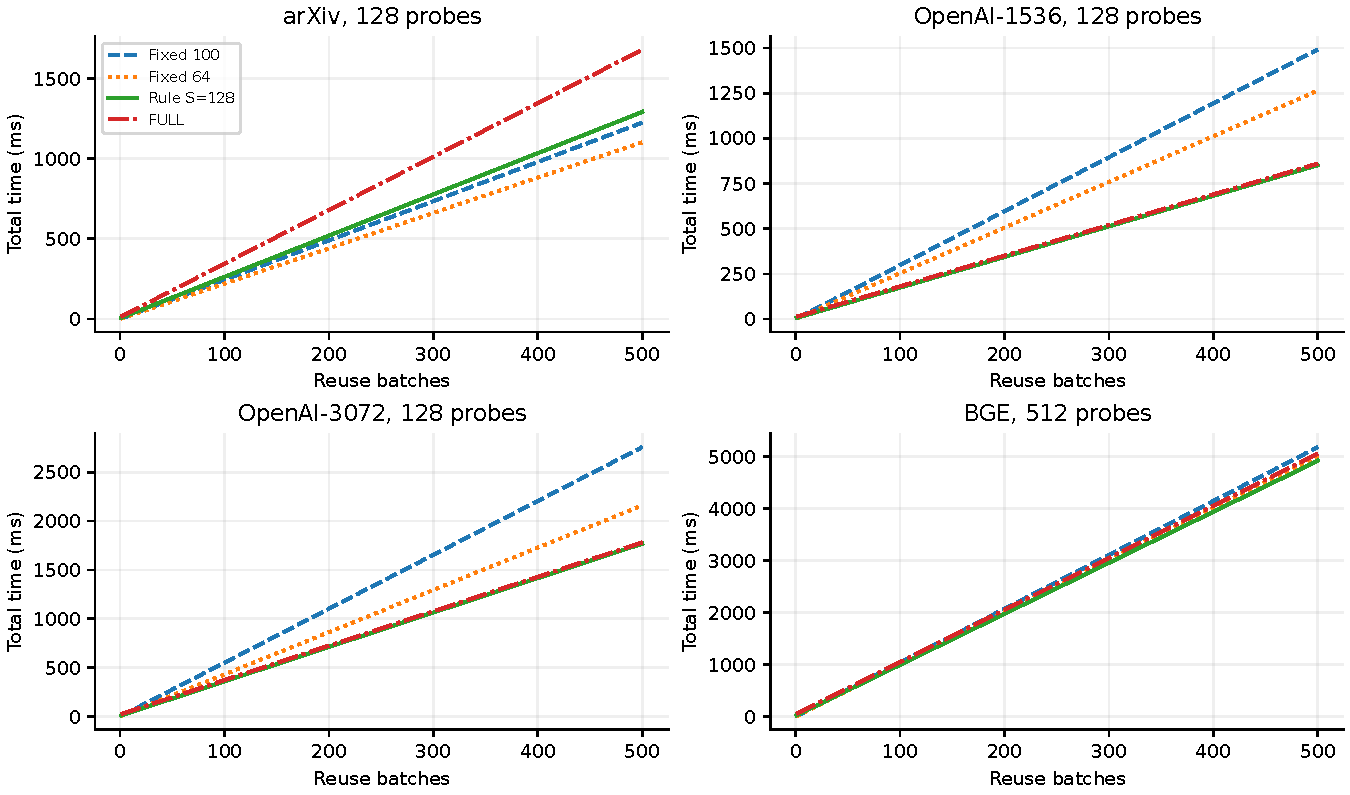
\includegraphics[width=\linewidth]{supplement/stream-cost.pdf}
\captionof{figure}[Direct cumulative calibrated-reuse time]{Direct mean cumulative time, including budget calibration and
first-batch setup. Each curve replays one fixed held-out query pool.
Policies can have different recall; timings alone are not a quality-matched
ranking. Dataset/probe settings match \cref{tab:7-stream-cost}.}
\label{fig:7-stream-cost}
\end{minipage}\par\medskip


\section{Batch Size, Scheduling and Workload Imbalance}
\label{sec:7-6}

Within the checked configurations, scheduling introduces no non-tie
primary-shortlist difference or final-ID-set difference across
250 variant/configuration pairs and 234,320 query comparisons. Tied
primary membership or output order can differ. Performance depends on
batch size: the integrated scheduler gains $2.727\times$ at batch 8 and
$1.015\times$ at batch 1,000 on average against the lane-refined
one-block baseline (\cref{tab:7-scheduling}). These averages do not
mean that every configuration improves.

\subsection{Parallelism versus repeated selection work}

Fixed eight-group scanning gains $2.06$--$2.76\times$ at batch 8.
For arXiv, scan time falls from 849 to 216\,$\mu$s, with another
16.7\,$\mu$s for merging. At batch 1,000 and $\alpha=200$,
independent-bound grouping instead raises scan time from 3,530 to
7,652\,$\mu$s and adds 2,624\,$\mu$s of merging, reaching only
$0.46\times$ one-block QPS. Shared bounds reduce maintenance work
without removing the cost of excessive grouping (\cref{fig:7-batch}).

\begin{figure}[!htbp]
\centering
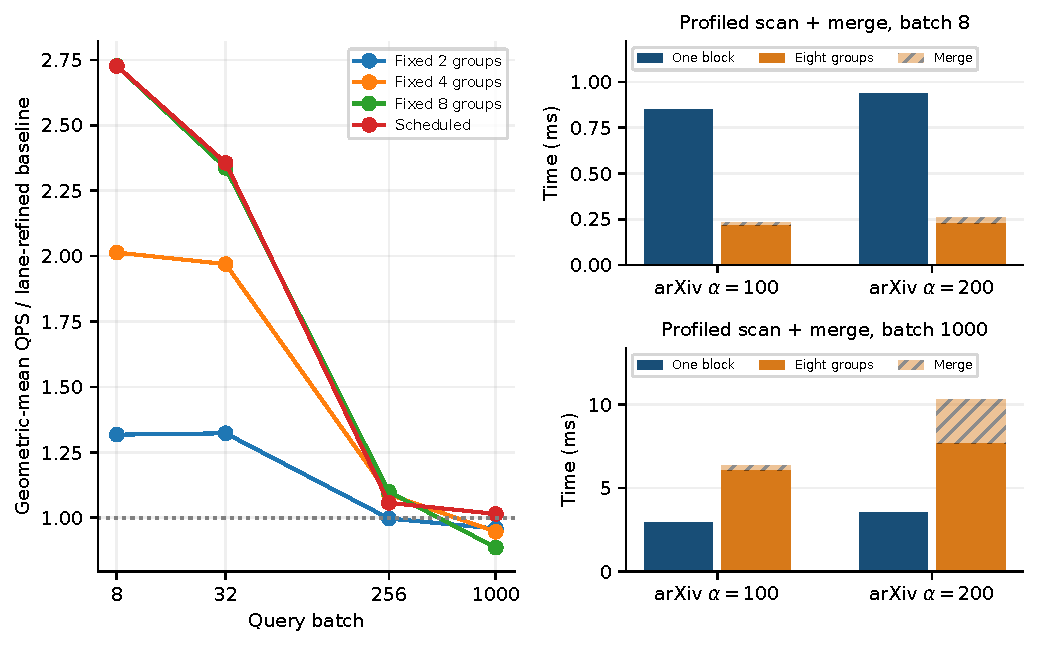
\includegraphics[width=\linewidth]{ch7/batch_execution.pdf}
\caption[Batch-dependent execution regimes]{Execution regimes. Left: fixed shared-bound group counts and
scheduled execution relative to the lane-refined one-block baseline
(13 settings at small batches, 11 at batch 1,000). Right: paired scan and
merge profiles at batches 8 and 1,000 for arXiv budgets 100 and 200.
Hatching denotes merge time. The right panels use the independent-bound
scan experiment; they explain a cost, not the scheduler's entire speedup.}
\label{fig:7-batch}
\end{figure}

\subsection{A fixed rule evaluated on further configurations}

The rule's constants were fixed on four configurations before testing
the others (\cref{sec:5-5}).

\begin{table}[!htbp]
\centering
\caption[Integrated execution and scheduling gains]{Integrated execution gains over the one-block, sixteen-lane baseline. Entries are geometric
 means of per-configuration median paired speedups from five rounds. ``Held out''
 excludes the four configurations used to set the rule; it means held-out
 configurations, not the budget experiment's held-out query split.}
\label{tab:7-scheduling}
\small\setlength{\tabcolsep}{4pt}
% Generated by scripts/build_ch7.py; do not edit numbers manually.
\begin{tabular}{@{}rrrrrrr@{}}
\toprule
Batch & Cells & $g_s=2$ & $g_s=4$ & $g_s=8$ & Scheduled & Held out \\
\midrule
8 & 13 & 1.318 & 2.014 & 2.728 & 2.727 & 2.930 \\
32 & 13 & 1.323 & 1.970 & 2.337 & 2.356 & 2.560 \\
256 & 13 & 0.997 & 1.090 & 1.099 & 1.057 & 1.041 \\
1000 & 11 & 0.959 & 0.947 & 0.886 & 1.015 & 1.012 \\
\bottomrule
\end{tabular}

\end{table}

The averages cover thirteen small-batch and eleven full-batch settings,
with 999 queries for Stella. Excluding the four rule-setting
configurations leaves nine and seven, respectively
(\cref{tab:7-scheduling}). At batch 1,000, fixed eight-group execution
averages $0.886\times$ the baseline. Relative to the best fixed choice,
the scheduler takes up to 1.217 times as long, on BGE at batch 256.

Vogue illustrates why candidate-count variation is an incomplete signal.
Its CV of 0.338--0.622 selects four groups even at batch 1,000.
Scheduled/one-block ratios range from 0.895 to 1.175, with losses at
low probe counts when the total work is too small to repay grouping.
The same choice enables the recall-0.97 advantage, but the rule does not
explicitly estimate scan volume or merging cost (\cref{sec:7-2}).

\section{Index Construction, Resident Memory and Tested Scale}
\label{sec:7-7}

JHQ-GPU builds and searches the largest tested dataset on one GPU:
Stella's 17.78 million vectors occupy 20.44\,GiB during search.
RQ1 is evaluated through separate construction, resident-memory and
completed-search measurements; the allocation comparison also informs
RQ4.

\subsection{Fresh indexes and input-loading cost}

Construction is index-cold: no trained-state cache is reused. The normal
build measurements use input files already in the operating system's
page cache, and time the train and add calls, not file loading or full
process startup. Three repeats give Vogue 298--303\,ms training and
$\approx0.56$\,s total; Stella takes 10.54--10.65\,s
(\cref{tab:7-build-memory}).

\begin{table}[!htbp]
\centering
\caption[Cold construction and resident memory]{Cold JHQ construction and separately measured resident memory.
Train/add are component medians of three supplementary normal builds;
Total is the median paired sum. Memory comes
from the table-sweep implementation's two-group, 128-probe, $\alpha=100$ runs and includes context
and workspace. ``Residual'' is the modelled residual-code share of the
measured used total, not the fraction read per query.}
\label{tab:7-build-memory}
\small\setlength{\tabcolsep}{3pt}
% Generated by scripts/build_ch7.py; do not edit numbers manually.
\begin{tabular}{@{}lrrrrrr@{}}
\toprule
Dataset & Train s & Add s & Total s & Used GiB & Raw GiB & Residual \\
\midrule
Vogue & 1.06 & 0.27 & 1.33 & 1.47 & 2.67 & 45.4\% \\
arXiv & 0.59 & 0.52 & 1.10 & 2.58 & 6.45 & 62.5\% \\
OpenAI-1536 & 0.64 & 0.38 & 1.01 & 2.39 & 5.72 & 59.7\% \\
OpenAI-3072 & 1.34 & 0.65 & 1.99 & 4.14 & 11.43 & 69.0\% \\
BGE & 3.75 & 3.67 & 7.42 & 11.93 & 38.50 & 80.7\% \\
Stella & 3.74 & 6.67 & 10.40 & 20.44 & 67.81 & 82.9\% \\
\bottomrule
\end{tabular}

\end{table}

The construction comparison in \cref{fig:7-build} uses the timing boundaries
in \cref{sec:3-3,sec:a-e1-protocol}.

\par\medskip\noindent\begin{minipage}{\linewidth}
\captionsetup{hypcap=false}
\centering
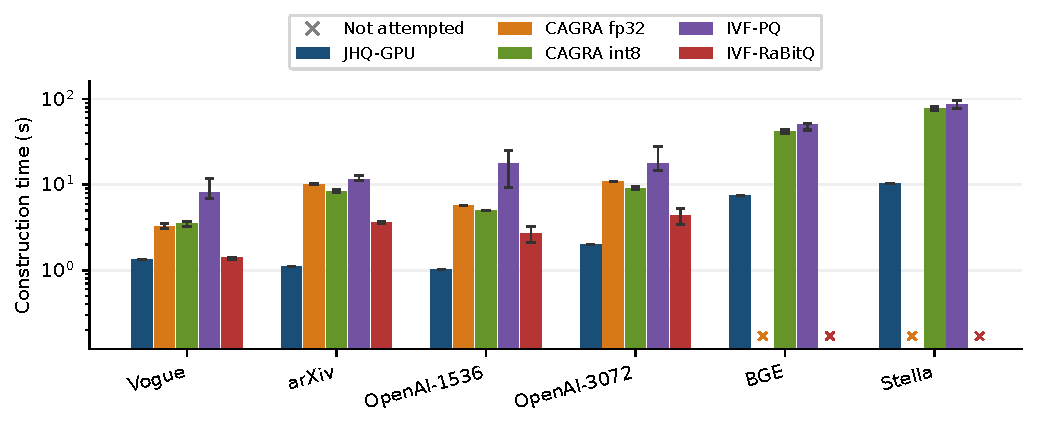
\includegraphics[width=\linewidth]{ch7/construction.pdf}
\captionof{figure}[Recorded construction costs]{Recorded construction costs, with CAGRA int8 included. JHQ is
the median and range of three supplementary normal cold builds with warm
input pages; other bars are medians across successful
measured index configurations, with minimum--maximum whiskers. Int8
includes dataset quantization; RaBitQ excludes the required serialization
round trip. Missing large-dataset bars denote unattempted configurations,
not measured build failures. The vertical axis is logarithmic.}
\label{fig:7-build}
\end{minipage}\par\medskip

Stella's two isolated CAGRA int8 settings take 74.55 and 82.45\,s,
including quantisation; IVF-PQ has a median 86.59\,s across three
configurations, compared with JHQ's 10.54--10.65\,s. These are
construction comparisons rather than equal-quality, equal-memory
search points.

Repeated training changes arXiv recall by at most 0.0012 across five
builds. Stella takes 18.2--18.6\,s from startup to searchable state with
warm input pages, and 129.9\,s on the session's first read. These wider
boundaries include input loading and startup, explaining why they exceed
train-plus-add time. Memory sampled every 20\,ms peaks at 26.08\,GiB
for BGE and 22.58\,GiB for Stella. BGE's 12\,GiB assignment buffers are
released before the 23.05\,GiB gather payload, so the two allocations
must not be added into one simultaneous peak
(\cref{eq:4-assignment-scratch}).

\subsection{Resident allocation and where compression helps}

Compression makes the large resident indexes feasible, but residuals
still dominate their storage. \Cref{fig:7-memory} combines the component
model in \cref{sec:4-4} with measured totals, retaining the unattributed
remainder.

\par\medskip\noindent\begin{minipage}{\linewidth}
\captionsetup{hypcap=false}
\centering
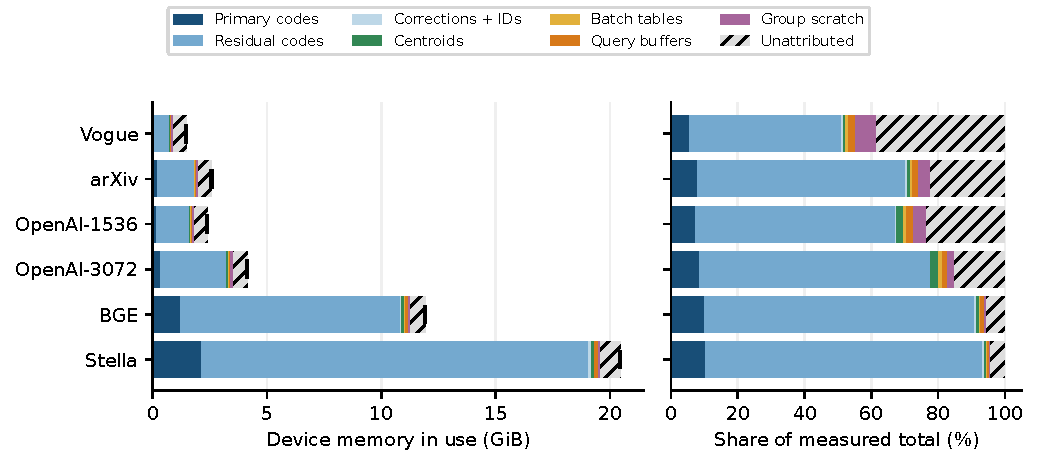
\includegraphics[width=\linewidth]{ch7/memory.pdf}
\captionof{figure}[Resident-memory decomposition]{Resident-memory decomposition at two-group tables, 128 probes
and $\alpha=100$. Component sizes are modelled, markers are measured used
totals, and hatching is the unattributed remainder. The totals include
context and workspace. The preceding construction measurements give sampled peaks; these
resident markers are not peaks.}
\label{fig:7-memory}
\end{minipage}\par\medskip

Residuals occupy 80.7\% of BGE's 11.93\,GiB and 82.9\% of Stella's
20.44\,GiB, including context and workspace. Their raw FP32 vectors
would require 38.50 and 67.81\,GiB, respectively. Lowering $\alpha$
saves residual reads, not the stored residual bytes.

The cross-system allocations use a different boundary
(\cref{tab:7-e1-memory}). Subtracting a 507.2\,MiB CUDA-context estimate
from JHQ's process total gives a net process allocation approximately
0.29--0.39 of CAGRA fp32's index allocation. JHQ still includes query
workspace, while CAGRA reports its build-time index delta. CAGRA int8
allocations are of a similar order to JHQ's. These are parameter-sweep
ranges rather than memory-matched recall points or equal peak budgets;
\cref{tab:4-bytes} gives the component model.

\par\medskip\noindent\begin{minipage}{\linewidth}
\captionsetup{hypcap=false}
\centering
\captionof{table}[Memory allocations in the main comparison]{Memory allocations in the main comparison. JHQ is process total minus a 507.2\,MiB
context estimate, including query workspace; both CAGRA columns are index
allocations measured during build. Ranges cover the parameter sweep.}
\label{tab:7-e1-memory}
\footnotesize\setlength{\tabcolsep}{4pt}
% Generated by scripts/build_ch7.py; do not edit numbers manually.
\begin{tabular}{@{}lrrr@{}}
\toprule
Dataset & JHQ net process GiB & CAGRA fp32 index GiB & Ratio range \\
\midrule
Vogue & 0.90--1.01 & 2.89--2.91 & 0.31--0.35 \\
arXiv & 2.01--2.19 & 6.84--6.98 & 0.29--0.32 \\
OpenAI-1536 & 1.79--2.33 & 5.95--5.97 & 0.30--0.39 \\
OpenAI-3072 & 3.54--3.82 & 11.67--11.68 & 0.30--0.33 \\
\bottomrule
\end{tabular}

\end{minipage}\par\medskip

\subsection{Large-dataset feasibility and competitive regions}

JHQ reaches higher measured recall than the successful compressed
baselines on both large datasets, while CAGRA int8 leads in part of
the lower-recall region (\cref{fig:7-large}). BGE has 10,091,524 vectors
and Stella 17,776,615; both use 1,024 dimensions and 32,768 IVF lists.
Stella uses held-out corpus queries, whose evaluation scope is defined
in \cref{sec:3-2}.

Full-precision CAGRA, RaBitQ and FP32 brute force were not attempted
where predicted storage exceeded device capacity. Their missing points
are planned exclusions, not measured out-of-memory or recall failures.

\par\medskip\noindent\begin{minipage}{\linewidth}
\captionsetup{hypcap=false}
\centering
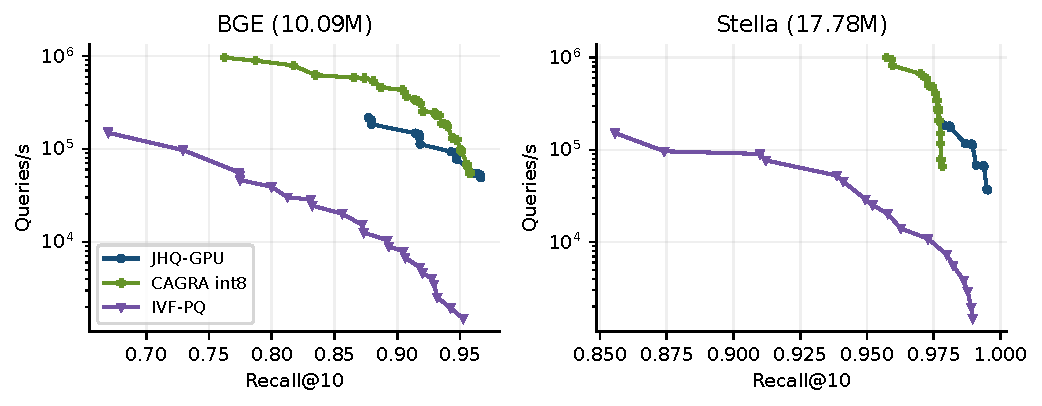
\includegraphics[width=\linewidth]{ch7/large_frontiers.pdf}
\captionof{figure}[Large-dataset search frontiers]{Large-dataset host-to-host frontiers, including the successful
isolated CAGRA int8 reruns. BGE/Stella use 1,000/999 queries. Endpoints mark tested-grid coverage.}
\label{fig:7-large}
\end{minipage}\par\medskip

CAGRA int8 fits Stella. On BGE it is $1.35$--$2.96\times$ faster at
recall 0.88--0.95, while JHQ is $1.086\times$ faster at int8's highest
recall, 0.9579. The respective maximum recalls on BGE and Stella are
0.9579 and 0.9783 for int8, 0.9663 and 0.9952 for JHQ, and 0.9525 and
0.9896 for IVF-PQ.

On Stella, JHQ gives 185.4 kQPS at recall 0.978679 versus int8's
66.3 kQPS at 0.978278. This $2.80\times$ ratio compares nearby measured
points, not equal recall; int8 has no measured coverage of the upper
region.

\section{Numerical Checks and Recall Analysis}
\label{sec:7-8}

\subsection{Quality resolution and repeated execution}

The recall-0.97 ranking survives a check that reduces the influence of
slow RaBitQ calls, but near ties remain sensitive to numerical and
measurement resolution. One ground-truth hit changes Recall@10 by
\[
 \Delta r=\frac1{nk}=
 \begin{cases}10^{-4},&n=1000,\\2\times10^{-4},&n=500.\end{cases}
\]
Stella's $n=499$ step is slightly larger; these steps are measurement
resolution, not uncertainty intervals.

Near recall 0.97, local slopes correspond to 1.01--3.17\% QPS change
per $10^{-3}$ recall before the interpolation tolerance is applied.
Five-build recall ranges are 0.0008 on Vogue, 0.0012 on arXiv,
0.0004 on OpenAI-1536 and 0.0002 on OpenAI-3072. They indicate local
sensitivity rather than bound a fully retrained frontier.
Cached-model FP32 comparisons remain favourable on OpenAI
(\cref{sec:7-precision}); the arXiv and LUT near ties are inconclusive.

RaBitQ's median five-round QPS ranges are 3.79\% on Vogue, 3.34\% on
arXiv, 2.87\% on OpenAI-1536 and 5.25\% on OpenAI-3072. These are
observed spreads, not confidence intervals. To test the influence of
occasional 30--60\,ms calls, the 1,000-query rate is recomputed as
$10^6/\operatorname{median}(\text{call ms})$ rather than using the mean
call time. At recall 0.97 the JHQ/RaBitQ ratios become 1.063, 0.995,
1.118 and 1.100, respectively: the three favourable directions and
arXiv near parity remain.

Vogue's recall varies between 0.9642 and 0.9644 across identity and
timing runs, including runs of the baseline itself. A separate
cross-binary identity check finds byte-identical probe and primary dumps
on 1,000 queries despite different final recall. These observations
remain unresolved; within-process selection checks do not explain the
cross-process variation (\cref{app:reproducibility}).

\subsection{Reconstructed scores and recall loss}
\label{sec:7-recall-attribution}

The reconstruction pilot quantifies a small remaining budget-related
gap in the checked cases, while routing and representation remain a
joint limitation. Across seven workload--budget settings with 128 queries
each, scoring all probed candidates in FP64 improves recall over the
GPU's selected-budget outputs by 0--0.002344. On arXiv at 128 probes,
$\alpha=200$ returns the same answer set as full-probe reconstructed
scoring on all 128 queries. At budget 100, recall is 0.9734375 versus
0.9750 for full-probe scoring: a difference of 0.0015625 alongside a
joint routing/reconstruction deficit of 0.0250 (\cref{sec:6-2}).

This example does not separate routing from reconstruction, and other
settings also mix FP64/GPU arithmetic differences into the comparison.
A complete attribution needs fixed queries and candidates with
stage-wise ground-truth coverage. The stage checks in
\cref{tab:5-query-stages} establish computed-score selection correctness
rather than raw-space exact nearest neighbours.

\chapter{Discussion and Future Work}
\label{ch:discussion}
\chaptermark{Discussion and Future Work}

This chapter explains when compression and parallel execution help,
why several alternative designs were rejected, and which experiments
could improve the system.

\section{Design Implications}
\label{sec:8-1}
\subsection{Index residency and construction workspace}

Compression determines whether an index can remain on the GPU, but
construction has its own capacity constraint. BGE occupies 11.93\,GiB
during search yet reaches a sampled 26.08\,GiB during construction.
Assignment buffers cause this peak before the gather buffers are
allocated. The two-pass build limits gather storage; it does not remove
all other temporary allocations. Feasibility therefore requires both
a resident-byte model and a phase-by-phase allocation model
(\cref{sec:4-5,sec:7-7}).

\subsection{Codebook structure and lookup cost}

The smallest table is not the fastest. Four- and eight-way splitting
store 16 entries per subspace, compared with 32 for the two-way split,
but need more lookups and additions. Two tables are fastest in 22 of
24 settings (\cref{sec:7-3}). Likewise, removing the table altogether
saves shared memory but loses speed in the earlier tests summarised in
\cref{tab:8-stopped}. The useful comparison is therefore reconstruction quality at the actual
GPU scoring cost.

\subsection{Parallelism must repay selection and merging}

Small batches leave too few independent queries to fill the GPU.
Splitting each query across blocks supplies more work, but repeats table
staging and local selection and adds a merge. Eight groups gain
$2.06$--$2.76\times$ at batch 8; at batch 1,000, independent-bound
grouping falls to $0.46\times$ one-block throughput in the profiled
high-budget case (\cref{sec:7-6}). This does not mean that large batches
should always use one block: grouping also handles uneven workloads,
and supplies Vogue's lead at recall 0.97. Its 0.895 throughput ratio on
a low-probe setting shows the rule's limit. The spread of candidate
counts does not measure their total volume; a better scheduler would
price scan, selection and merge work together.

\subsection{Selection correctness and search quality}

Exact selection of computed scores is a separate requirement from
finding the nearest original vectors. The grouped selector's proof and
CPU sorting checks establish that parallel decomposition retains the
specified primary shortlist (\cref{sec:5-4,sec:7-strict-selection}).
They do not remove IVF routing losses or quantisation error. Testing
these layers separately distinguishes an implementation defect from a
limitation of the representation or refinement budget.

\subsection{Refinement speed and budget savings}

How much a smaller budget saves depends on the rest of the search.
Let $T_0>0$ be fixed non-refinement time, $F_h\geq F_\ell>0$ the
refinement times at high and low budgets, and $\eta\in(0,1]$ a common
multiplier that makes both refinement kernels faster. The low-budget
speedup and its derivatives are
\begin{align}
 S(\eta,T_0)&=\frac{T_0+\eta F_h}{T_0+\eta F_\ell},
 \label{eq:8-refinement-sensitivity}\\
 \frac{\partial S}{\partial\eta}
 &=\frac{T_0(F_h-F_\ell)}{(T_0+\eta F_\ell)^2}\geq0,\qquad
 \frac{\partial S}{\partial T_0}
 =\frac{\eta(F_\ell-F_h)}{(T_0+\eta F_\ell)^2}\leq0.\nonumber
\end{align}
For $F_h>F_\ell$, reducing $\eta$ reduces the relative benefit of
cutting the budget, whereas reducing $T_0$ increases it. This model
explains why kernel optimisation and budget reduction cannot be treated
as independent multiplicative gains. It assumes the same refinement
speedup at both budgets and fixed non-refinement work. Actual scan
maintenance can change with the budget, so adoption still depends on
measured total time and quality (\cref{sec:7-5,sec:7-stream-cost}).


\section{Alternative Scoring and Coding Experiments}
\label{sec:8-2}
\subsection{Mailman-style shared-sum scoring}
\label{sec:8-mailman}

JHQ's finite sign patterns suggest reusing partial sums across
candidates, following the Mailman idea \cite{mailman}. A four-bit half-code
has only 16 patterns, so many candidates can share intermediate work.
The test freezes the primary codes and candidate streams on Vogue,
arXiv and OpenAI-3072. Atomic buckets and private histograms at group
widths 4, 6 and 8 are compared with packed two-table scoring, using
128 probes and batches of 8 and 1,000.

The best replacement reaches only 0.187--0.581 of the scorer baseline's
throughput. Profiles show concentrated bucket updates, while private
histograms introduce more state and shared-memory updates. Arithmetic
reuse is insufficient when obtaining it costs more than the saved
lookup work. These are scorer measurements, not an integrated search
comparison. If $f$ is the baseline time fraction spent scoring and $s$
the replacement's relative scorer speed, the unchanged-rest model gives
\[
 \frac{T'}T=1+f\left(\frac1s-1\right)>1
 \quad(0<f\leq1,\ 0<s<1).
\]
Thus even this model predicts no whole-search gain. Integration stopped;
other finite-alphabet implementations remain possible. The left panel
of \cref{fig:8-negative} shows the six scorer comparisons.

\par\medskip\noindent\begin{minipage}{\linewidth}
\centering\captionsetup{hypcap=false}
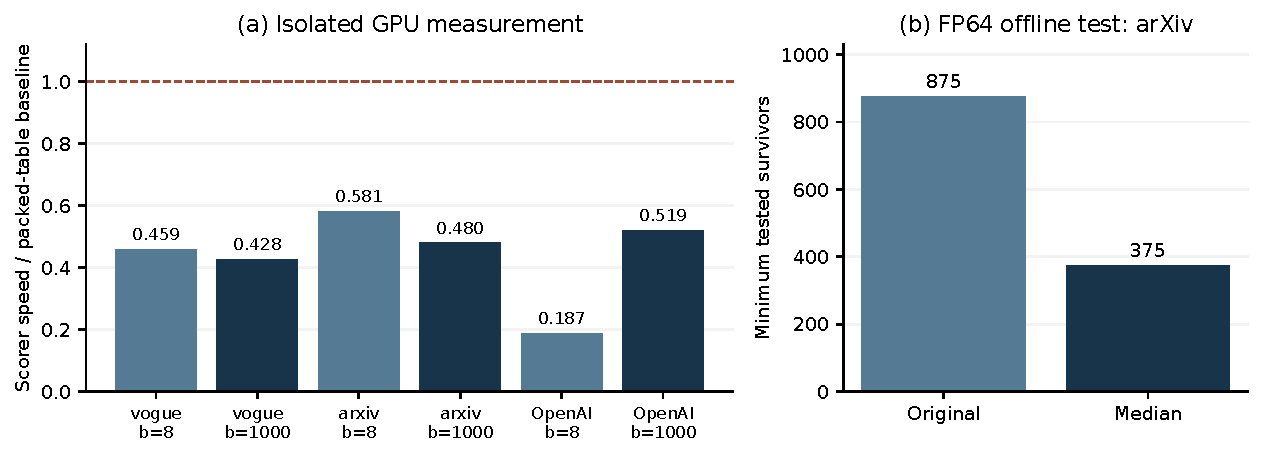
\includegraphics[width=\linewidth]{ch8/negative-evidence.pdf}
\captionof{figure}[Mailman and rank-oriented coding]{Mailman scorer throughput (left) and offline shortlist size (right).}
\label{fig:8-negative}
\end{minipage}\par\medskip

\subsection{Rank-oriented coding experiments}
\label{sec:8-rank}

Minimising reconstruction error need not preserve neighbour order.
FP64 offline replay tests weighted scores, median and list-dependent
thresholds, learned losses and linear minimum mean-square-error decoding,
with 400 calibration, 200 validation and 400 test queries. On arXiv,
median thresholds reduce the smallest tested shortlist reaching recall
0.97775 from 875 to 375 candidates; the other two workloads fail their
respective targets. These are the offline counts in the right panel of
\cref{fig:8-negative}.

A separate GPU follow-up changes the primary representation and retrains
the residual codes. At its own arXiv target of 0.9766, throughput improves
$1.40\times$ at batch 8 and $1.21\times$ at batch 1,000. Vogue instead
peaks at recall 0.9630, below its 0.9644 target, and OpenAI-3072 nearly
ties. The offline count reduction and GPU speedup use different queries,
states and targets; they do not establish a threshold-only speedup.
Changing primary codes also changes what the residuals must reconstruct.

\subsection{Removing a shared mean}
\label{sec:8-centring}

A global data mean can consume sign-code resolution. Rotation preserves
that mean's norm: for orthogonal $\Pi$,
\[
 \bar y=\frac1N\sum_i\Pi x_i=\Pi\bar x,
 \qquad \|\bar y\|^2=\bar x^\top\Pi^\top\Pi\bar x=\|\bar x\|^2.
\]
In real arithmetic, subtracting the same mean $\mu$ from queries and
database vectors preserves distances,
$\|(q-\mu)-(x-\mu)\|^2=\|q-x\|^2$,
but changes the quantisation problem.

A follow-up compares the archived original index with a fresh index
trained on centred data, alternating both in one session. On arXiv,
whose mean norm is 0.837, full-pool calibration at 128 probes changes
$\alpha=200$ to $\alpha=64$, and the recall-0.97 frontier improves
$1.266\times$. At 512 probes the selected budget becomes 100, not 64.
The change is not uniformly beneficial: Vogue's high-budget recall at
512 probes falls from 0.9918 to 0.9896, and OpenAI-1536's selected budget
rises from 8 to 16 despite a nearly unchanged recall-0.97 throughput
ratio of 0.995. The arXiv result supports mean removal as a useful
representation change. Retraining also changes centroids and residuals,
so repeated, equally retrained controls are needed to isolate its
contribution. These runs extend the analysis, not the main comparison
with other systems.

\subsection{A safe bound can still prune too little}
\label{sec:8-residual-bound}

A separate FP64 pilot constructs a lower bound on squared distance to
the reconstructed vector using only primary codes. For each sign
pattern, a box encloses residual coordinates from all indexed vectors.
Shifting it by the primary reconstruction gives a lower bound via
distance from the query. Across seven search
settings and 72.8 million candidate checks, no violation is observed.
Yet median bound-to-distance ratios are only 0.13--0.24. Even an ideal
final threshold leaves almost all probed candidates for refinement,
usually far more than the existing shortlist. The pilot therefore
stopped before an integrated GPU implementation. Safety alone is
insufficient: pruning must be selective enough to repay evaluating the
bound and reading surviving residuals. A GPU version would also need
rounding-safe envelopes.

\subsection{Further alternatives and stopping decisions}
\label{sec:8-stopped}

\Cref{tab:8-stopped} summarises representative earlier alternatives.
They use their own versions and controls rather than the final
cross-system protocol. GPU timings and offline cost estimates are
identified separately; the latter are not additional system-frontier
measurements.

\par\medskip\noindent\begin{minipage}{\linewidth}
\centering\captionsetup{hypcap=false}
\captionof{table}[Alternative designs and stopping decisions]{Alternative designs and stopping decisions.}
\label{tab:8-stopped}
\footnotesize\setlength{\tabcolsep}{4pt}
\begin{tabularx}{\linewidth}{@{}>{\raggedright\arraybackslash}p{.24\linewidth}>{\raggedright\arraybackslash}p{.24\linewidth}X@{}}
\toprule
Alternative & Expected saving & Evidence and decision \\
\midrule
Larger selection buffer & Fewer compaction sorts & GPU tests lose up to 24\% throughput; added shared memory reduces the possible resident blocks in affected cases \\
Fused scan and refinement & Fewer launches and intermediate transfers & GPU tests lose up to 15\%; the saved transfer is small relative to the combined kernel's resource demand \\
Partial-score early exit & Skip remaining subspaces & GPU changes range from $-2.8$ to $+4.2\%$; warp-wide checks give no consistent gain \\
Table-free sign scoring & Remove lookup-table storage & GPU throughput falls 30--52\% despite the smaller shared-memory footprint \\
Progressive primary reads & Read full codes only for survivors & Offline replay and traffic estimates expose scattered second-stage reads; no new GPU search kernel was timed \\
Local-first refinement & Avoid a global primary merge & Offline quota policies do not beat global selection at equal work; a favourable oracle allocation is unavailable online \\
\bottomrule
\end{tabularx}
\end{minipage}\par\medskip


\section{Threats to Internal and External Validity}
\label{sec:8-3}
\Cref{tab:8-threats} identifies how the main interpretations could fail
and which controls address them. Measurement definitions remain in
Chapter 3; repeated build and precision checks are in \cref{sec:7-8}.

\par\medskip\noindent\begin{minipage}{\linewidth}
\centering\captionsetup{hypcap=false}
\captionof{table}[Threats to validity]{Threats to validity and remaining checks.}
\label{tab:8-threats}
\footnotesize\setlength{\tabcolsep}{4pt}
\begin{tabularx}{\linewidth}{@{}*{3}{>{\raggedright\arraybackslash}X}@{}}
\toprule
Claim at risk & Alternative explanation & Control and remaining test \\
\midrule
Execution gain & Changed scores, ties or index state cause the apparent gain & CPU re-sorting and table-score checks; finite coverage, with candidate arrays requiring regeneration for further tests \\
Budget quality & Calibration samples miss difficult queries or the workload changes & Separate labelled test queries, recorded decision curves and full-pool enumeration; untested query subsets and future distributions remain \\
Competitive margin & Parameter grids, slow calls or interface overhead change the ranking & Both recall estimators, retained slow calls, int8 and precision checks; small-batch comparison; other devices untested \\
Capacity/build claim & Short-lived allocations escape peak sampling & Allocation lifetimes, repeated cold builds and 20\,ms memory sampling; shorter peaks and complete retrained frontiers remain unmeasured \\
\bottomrule
\end{tabularx}
\end{minipage}\par\medskip

The earlier CPU comparison in \cref{sec:7-cpu} establishes the observed
throughput difference at matched recall for historical implementations.
Separate training, unequal list counts on the OpenAI datasets and sparse
CPU timing repeats limit its interpretation. A comparison against the
evaluated GPU version with matched index and timing controls remains
unmeasured.

Six datasets do not represent six independent user workloads. The two
OpenAI exports share a DBpedia corpus, and Stella uses queries held out
from its corpus rather than the original query set (\cref{sec:3-2}).
The comparisons include transfers and host interfaces; differences in
memory types and C++ versus Python calling costs can affect small-batch
margins, so those margins cannot all be attributed to GPU search kernels
(\cref{sec:3-3}). Evidence covers one GPU, static indexes and squared-L2
top-10 search. Near duplicates may remain and relevance labels are
absent; updates, concurrent services, drift, billion-scale capacity and
multiple GPUs have not been evaluated.


\section{Future Research Directions}
\label{sec:8-4}
\subsection{Mean-aware representations}

The centring result suggests testing when the primary signs should
encode deviations from a mean (\cref{sec:8-centring}). Repeated cold
builds of centred and uncentred data should first separate this effect
from training variation. List-dependent means are another candidate,
but require consistent query scoring and residual reconstruction.
The test should compare shortlist coverage, the best attainable refined
recall, selected budgets and total throughput, so a cheaper shortlist
cannot conceal a lower quality ceiling.

\subsection{Calibration risk and reuse cost}

Can a statistically controlled budget choice save more query time than
it costs to obtain? Under the nesting conditions of
\cref{eq:6-rank-curve}, reference-neighbour primary ranks could replace
repeated trial searches. An earlier four-setting offline replay found
that sequential sampling added searches; a model fitted to measured
calibration times estimated higher cost despite fewer sampled queries.
It was not an integrated GPU controller measurement. A replacement
should test batched trials or rank reuse against a quality-matched fixed
budget using direct calibration-plus-reuse time. Its risk analysis must
cover the sampling and budget-selection procedure, and drift should
trigger renewal. Reference-relative control still needs a link to labels
to provide absolute recall guarantees.

\subsection{Residual storage across GPU and host memory}

Residuals account for 80.7--82.9\% of the total resident process memory
on BGE and Stella (\cref{sec:7-7}), but only shortlisted rows are read.
Keeping routing and primary codes on the GPU while fetching residual
blocks from host memory could increase capacity. The difficulty is
turning scattered shortlist positions into efficient block transfers.
Under fixed scoring and selection, vary the device budget and measure
extra bytes, cache hits, transfer overlap, throughput and tail latency.
This would establish the capacity--latency trade-off rather than assume
that offloading improves speed.

\subsection{Explaining the small-batch boundary}

At recall 0.97, grouping improves JHQ's small-batch execution yet does
not close the gap to CAGRA fp32 (\cref{sec:7-smallbatch}). Candidate
work, selection overhead and interface costs could each contribute.
A matched study should count candidates scored by both indexes and
separate kernel time from transfers and host-call overhead. Comparing
those costs across batches would test whether fewer probed candidates,
cheaper selection or a different index is the useful next step.


\section{Deployment Considerations}
\label{sec:8-5}
The tested results make JHQ-GPU a candidate for memory-limited,
batch-throughput workloads near recall 0.97 (\cref{sec:7-2,sec:7-7}).
They do not establish a uniform advantage up to that recall: compressed
baselines win some lower-recall regions, and CAGRA fp32 wins at batch 8
and recall 0.97. For a stable workload, the tested 500-query calibration
is a useful initial setting, followed by an independent quality check
and a comparison of total reuse time with a fixed budget. Changes to
the index or query distribution require renewed validation.


\chapter{Conclusion}
\label{ch:conclusion}

\section{Answers to the Four Research Questions}
\label{sec:9-1}

\paragraph{RQ1: GPU index construction and capacity.}
A complete JHQ index can be built and searched on one GPU without keeping
the raw database vectors on the device. Training and encoding run on the
GPU, with bounded batches and a two-pass build controlling temporary
storage. Stella's 17.78 million vectors require 67.81\,GiB in FP32;
JHQ-GPU's resident process occupies 20.44\,GiB, including context and
workspace. Index-cold construction takes 10.54--10.65\,s, with a sampled peak of
22.58\,GiB on the 32\,GB device (\cref{sec:7-7}).

\paragraph{RQ2: Representation-aware execution.}
JHQ's code structure supports small lookup tables, contiguous reads and
parallel candidate selection. Splitting each 256-entry primary table
into two 16-entry tables preserves the real-arithmetic score and is the
fastest tested table form in 22 of 24 settings. Packing codes into words
makes adjacent scanning threads read consecutive memory, while threads
can cooperate to refine one candidate. For small batches, splitting a
query across blocks adds useful parallelism: scheduling gives
$2.727\times$ throughput at batch 8 relative to the single-block baseline
with cooperative refinement. Grouped selection matches a CPU sort of the
GPU-computed scores in all 55,296 checked query instances; single-block
differences occur only at tied cut-offs
(\cref{sec:7-3,sec:7-6,sec:7-strict-selection}).

\paragraph{RQ3: Workload-level refinement calibration.}
Unlabelled queries can select a reusable refinement budget that meets
the tested quality target, but sample size matters. Using all 500
calibration queries keeps held-out recall within $10^{-3}$ of the
highest measured recall across tested budgets in all twelve settings;
the maximum observed loss is 0.0006. Smaller samples can miss queries
that need more refinement: with 128 queries, arXiv exceeds the target
in 40 of 64 calibration samples at 128 probes and 32 of 64 at 512 probes. With 128-query calibration, direct OpenAI tests recover overhead
within 4--9 batches relative to the fixed-budget controls. On arXiv, the selected budget instead
spends more time to reach the quality target (\cref{sec:7-5}).

\paragraph{RQ4: Cross-system search performance.}
The main comparison favours JHQ-GPU at high batch throughput. At recall
0.97 and batch 1,000, it delivers $1.32$--$1.75\times$ the throughput of
CAGRA fp32 across four datasets. Across the tested grid, net process memory excluding CUDA context is
0.29--0.39 of CAGRA's index allocation. It leads the tested methods on Vogue and
both OpenAI datasets, while arXiv is nearly tied with IVF-RaBitQ;
Vogue's lead depends on grouped scanning (\cref{sec:7-2}). The OpenAI
measurements use TF32 multiplication; FP32 checks retain the lead over
CAGRA fp32 using the same trained model
(\cref{sec:b-precision-anchors}). This advantage has a batch-size boundary:
at batch 8 and recall 0.97, CAGRA fp32 is faster on all four datasets
(\cref{sec:7-smallbatch}).

\section{Contributions, Limitations and Outlook}
\label{sec:9-2}

Compression delivers capacity and speed when codes are cheap to access,
parallelism matches the batch and refinement meets the workload's
quality needs.

The evidence covers one GPU, six prepared datasets, squared-L2 top-10
search and static indexes. Historical CPU comparisons do not quantify a
speedup for the evaluated version (\cref{sec:7-cpu}). Reference agreement
on the calibration pool leaves future-query quality uncertain.

Two extensions follow. Risk-controlled calibration should account for
workload drift and expected reuse, and be compared with a quality-matched
fixed budget on total time, including calibration. Fetching residual
codes from host memory could expand capacity; transfer volume, overlap
and tail latency would determine when it pays off (\cref{sec:8-4}).


\clearpage
\bibliographystyle{plainnat}
\bibliography{references,variants/final-polish/references-extra}

\end{document}
